\chapter{Kolejowe, łukowe przęsła mostowe}
\section{Wstęp}


\section{Układ statyczny i konstrukcja mostów łukowych}

W celu łatwiejszego odbioru dalszych rozważań na wstępie przedstawiono klasyfikację mostów łukowych. Tradycyjnie mosty łukowe wykonywane były jako pełne sklepienia, ze ściankami czołowymi i z wnęką wypełnioną piaskiem, żwirem lub słabym betonem. Ukształtowany w ten sposób ustrój mógł być wykonany z tradycyjnych materiałów takich jak na przykład kamień \parencite{Szczygie1978}. Obecnie tego typu obiekty wykonuje się niezmiernie rzadko. Służyły one do przekraczania raczej niewielkich rozpiętości (do ok. 40 m) i w dzisiejszych czasach zostały wyparte głównie przez strunobetonowe konstrukcje prefabrykowane \parencite{Ciesla2013} i obiekty gruntowo-powłokowe \parencite{Janusz2009,Tomala2019}. Podobną formę geometryczną, ze ścianami czołowymi działającymi jako elementy konstrukcyjne stanowią łuki tarczowe. Obecnie mosty łukowe wykonuje się głównie w formie konstrukcji belkowo-płytowych. 


\subsubsection{Kształt i schemat statyczny konstrukcji}
Z punktu widzenia schematu statycznego dźwigara łukowego wyróżnia się łuki bezprzegubowe (utwierdzone), dwuprzegubowe i trójprzegubowe. Wybór schematu statycznego miał niegdyś większe znaczenie ze względu na różny stopień złożoności obliczeniowej układów. Obecnie obliczanie układów statycznie niewyznaczalnych nie stanowi problemu dzięki obliczeniom z wykorzystaniem MES. Dzięki temu bez popełnienia błędu obliczeniowego można wyeliminować z wnętrza konstrukcji przeguby, które z punktu widzenia trwałości konstrukcji są elementami niepożądanymi. Z drugiej strony, jak wiadomo układy statycznie wyznaczalne są odporne na obciążenia drugorzędne i należy je stosować w przypadku zagrożenia na przykład przemieszczenia podpór. Niezależnie od zmian w podejściu do projektowania aktualną pozostaje reguła przytoczona przez \cite{Pszenicki1954}: \textquote{Zasadą jest, że obliczenie powinno odpowiadać konstrukcji (...).}. Stąd wybór schematu statycznego musi odpowiadać nie tylko teoretycznym założeniom, ale możliwościom ukształtowania warunków brzegowych w rzeczywistej konstrukcji. 

Ze względu na wzajemne usytuowanie pomostu i dźwigarów łukowych można wyszczególnić następujące rodzaje konstrukcji:
\begin{itemize}[noitemsep]
	\item pomost usytuowany w całości nad łukiem - z jazdą górą (Rys. \ref{fig:bri_deck_loc_top}, \ref{fig:arch_deck_bridges_a}),
	\item pomost usytuowany w całości poniżej łuku - z jazdą dołem (Rys. \ref{fig:bri_deck_loc_middle}, \ref{fig:arch_deck_bridges_d}),
	\item pomost usytuowany pośrednio - z jazdą pośrednią (Rys. \ref{fig:bri_deck_loc_bott}, \ref{fig:arch_deck_bridges_e}).
\end{itemize}

\begin{figure}[hbt!]
	\centering
	\subfloat[most łukowy z jazdą górą]{\includegraphics[width=0.7\linewidth,page=4]{/mosty_wstep/mosty.pdf},\label{fig:bri_deck_loc_top}}  \\
	\subfloat[most łukowy z jazdą pośrednią]{\includegraphics[width=0.7\linewidth,page=6]{/mosty_wstep/mosty.pdf},\label{fig:bri_deck_loc_middle}} \\
	\subfloat[most łukowy z jazdą dołem]{\includegraphics[width=0.7\linewidth,page=5]{/mosty_wstep/mosty.pdf},\label{fig:bri_deck_loc_bott}}
	\captionsetup{justification=centering}
	\caption{Klasyfikacja mostów łukowych ze względu na wzajemne położenie pomostu i dźwigara}
	\label{fig:bridges_types_deck_location}
\end{figure}

%\begin{figure}[bt!]
%	\centering
%	\captionsetup{justification=centering}
%	
%	\subfloat[Wiadukt WK-11 w ciągu PKM Gdańsk (fot. materiały archiwalne firmy Keller)]{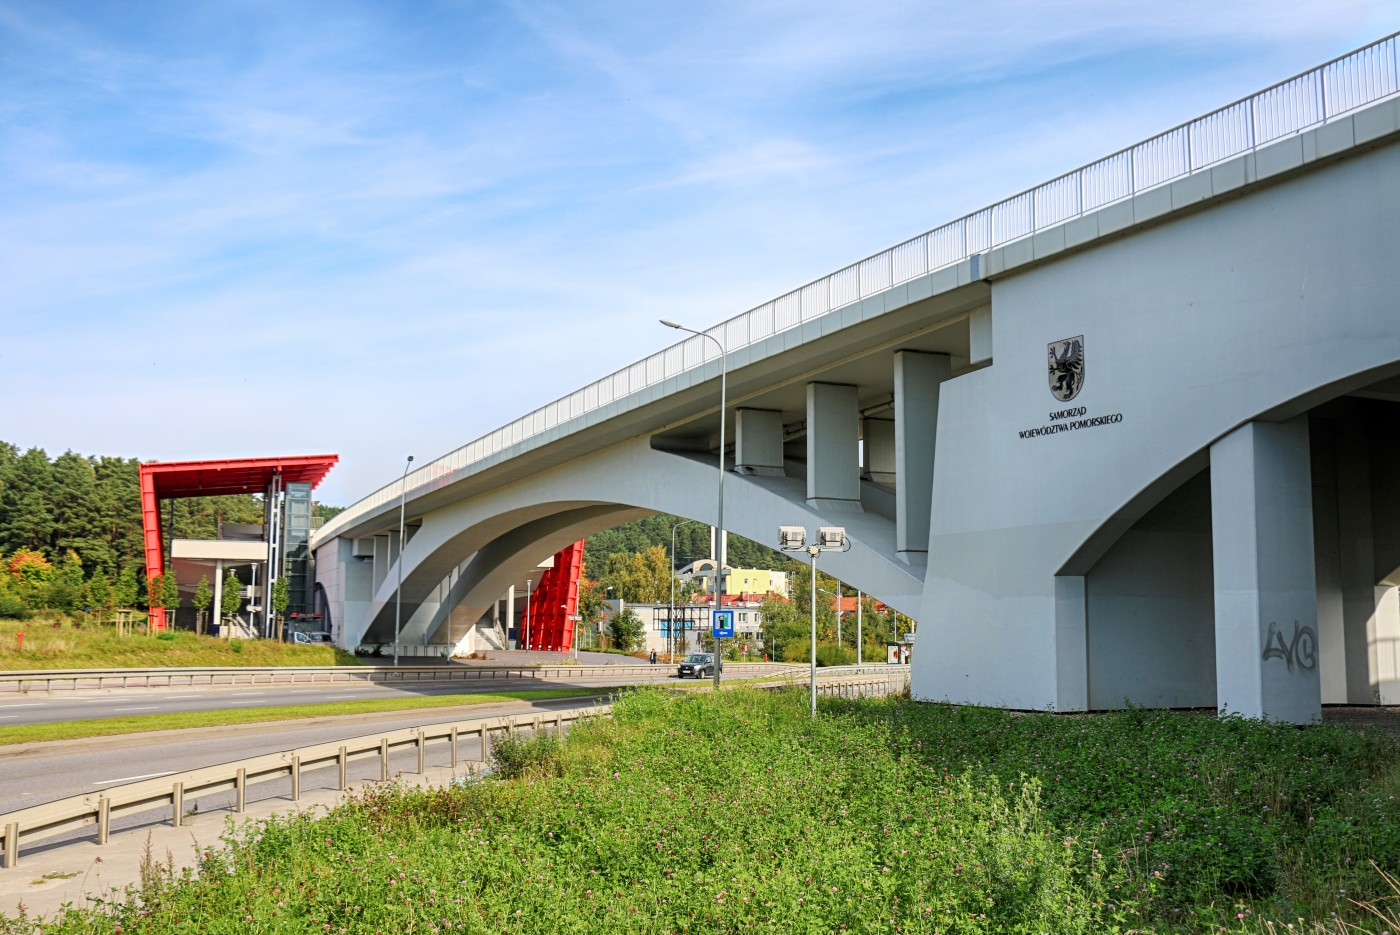
\includegraphics[width=0.48\linewidth]{/mosty_wstep/photos/keller-polska-pale-cfa-pkm-gdansk-8.jpg} \label{fig:arch_deck_bridges_a}} \;
%	%
%	\subfloat[Most im. Marszałka Piłsudzkiego w Krakowie (fot. Jakub Hałun/wikipedia.org)]{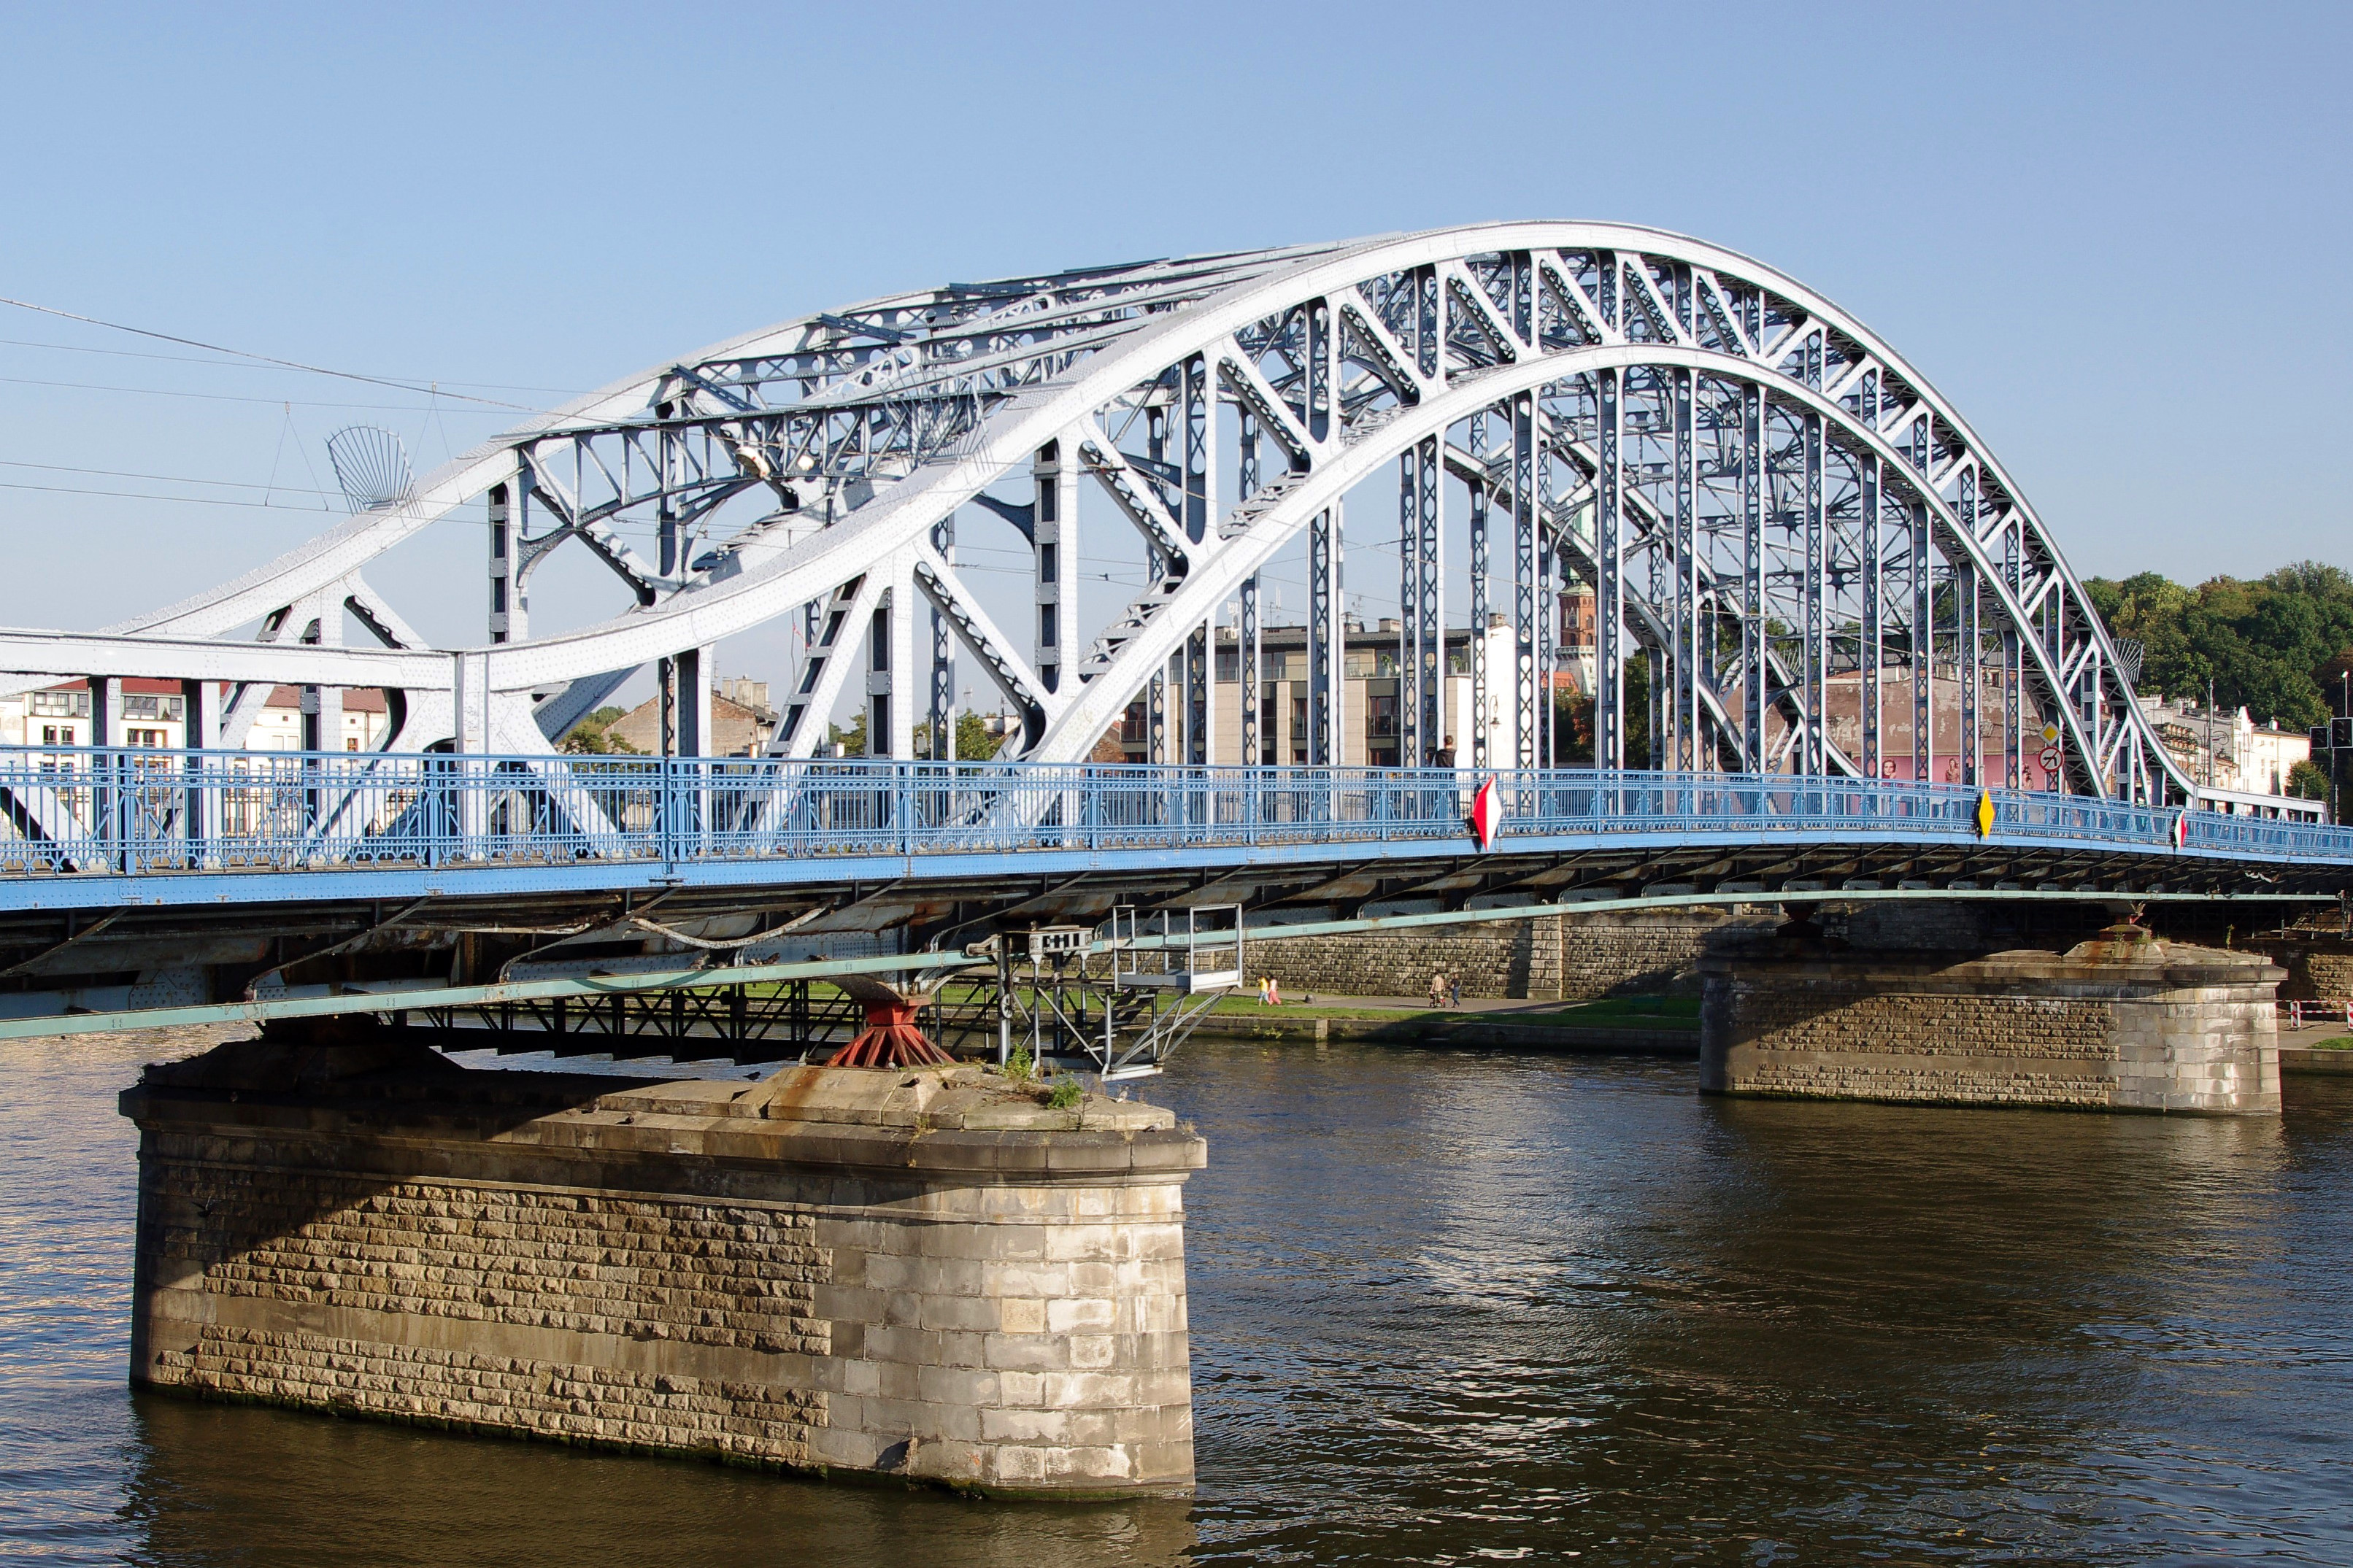
\includegraphics[width=0.48\linewidth]{/mosty_wstep/photos/Krakow_most_Pilsudskiego.jpg} \label{fig:arch_deck_bridges_b}} \\
%	%
%	\subfloat[Most im. Jana Pawła II w Puławach\\(fot. Kamil Lewandowski/Gmina Puławy)]{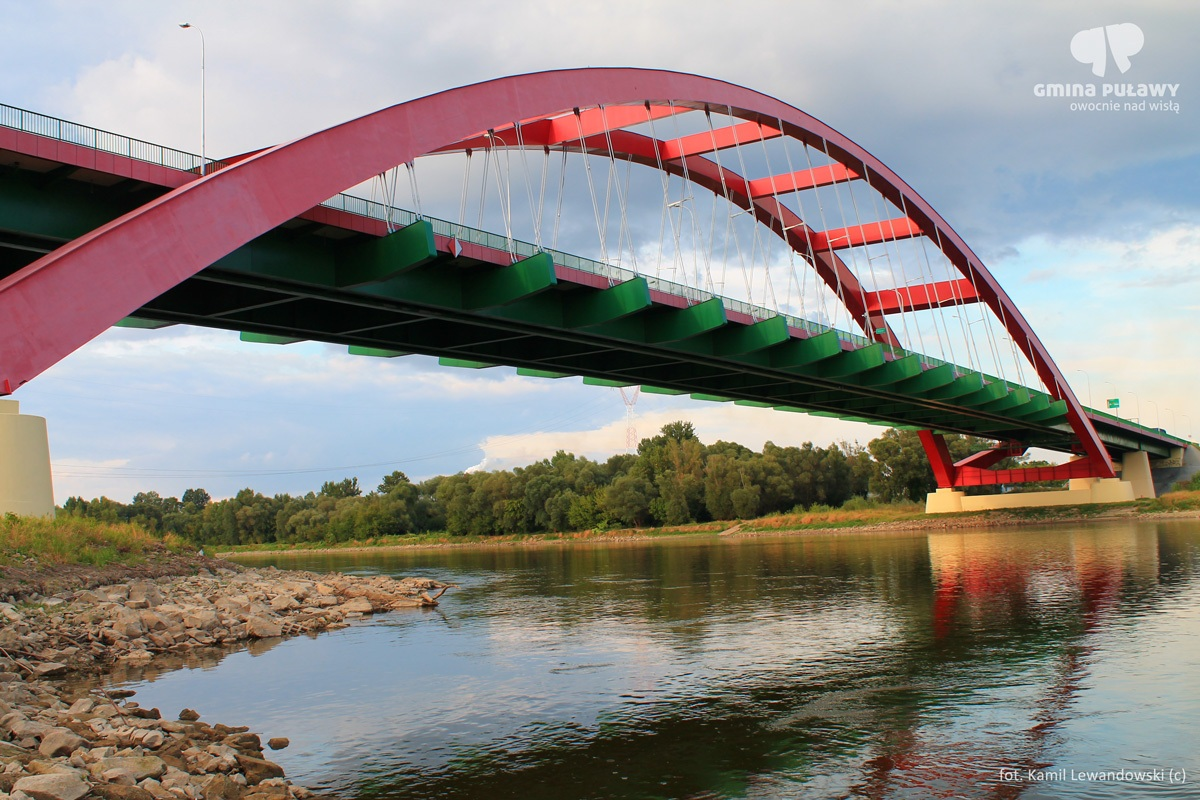
\includegraphics[width=0.48\linewidth]{/mosty_wstep/photos/most_pulawy.jpg} \label{fig:arch_deck_bridges_c}} \;
%	%
%	\subfloat[Most na Dziwnie w ciągu obwodnicy Wolina\\(fot. Radosław Drożdżewski)]{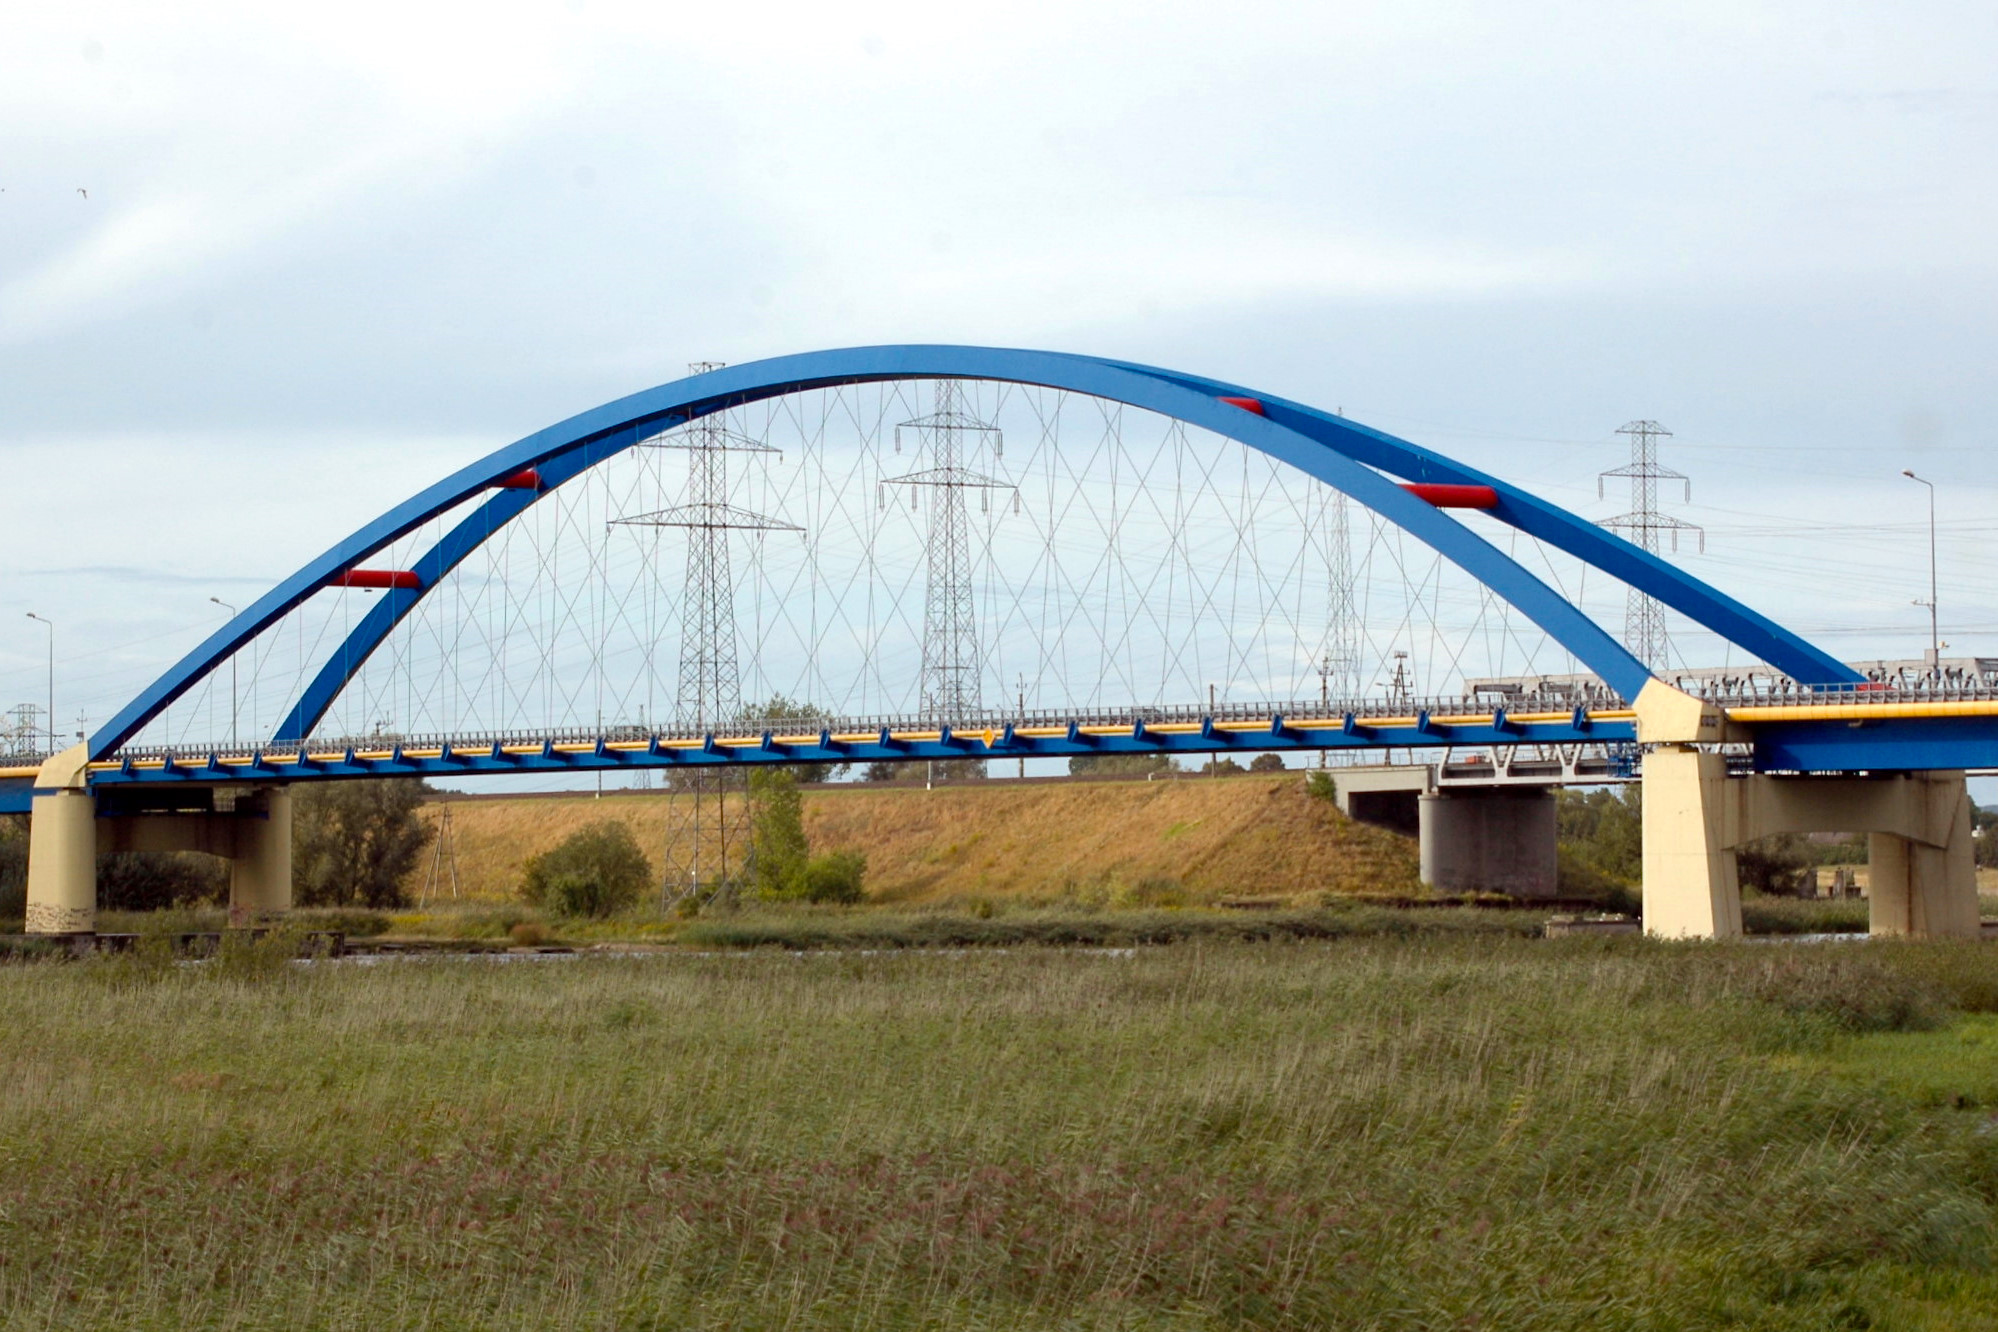
\includegraphics[width=0.48\linewidth]{/mosty_wstep/photos/Wolin_-_most_obwodowy_DK3_d_radoslaw_drozdzewski.jpg} \label{fig:arch_deck_bridges_d}}
%	%
%	\caption{Wybrane polskie mosty łukowe: (a) wiadukt z jazdą górą i dźwigarem żelbetowym, (b) most z jazdą dołem i dźwigarem kratowym, (c) most z jazdą pośrednią i dźwigarem stalowym, (d) most z jazdą dołem i dźwigarem stalowym}
%	\label{fig:arch_deck_bridges}
%\end{figure}

%\begin{figure}[p]
%	\centering
%	\captionsetup{justification=centering}
%	
%	\subfloat[Wiadukt WK-11 w ciągu PKM Gdańsk (arch. własne)]{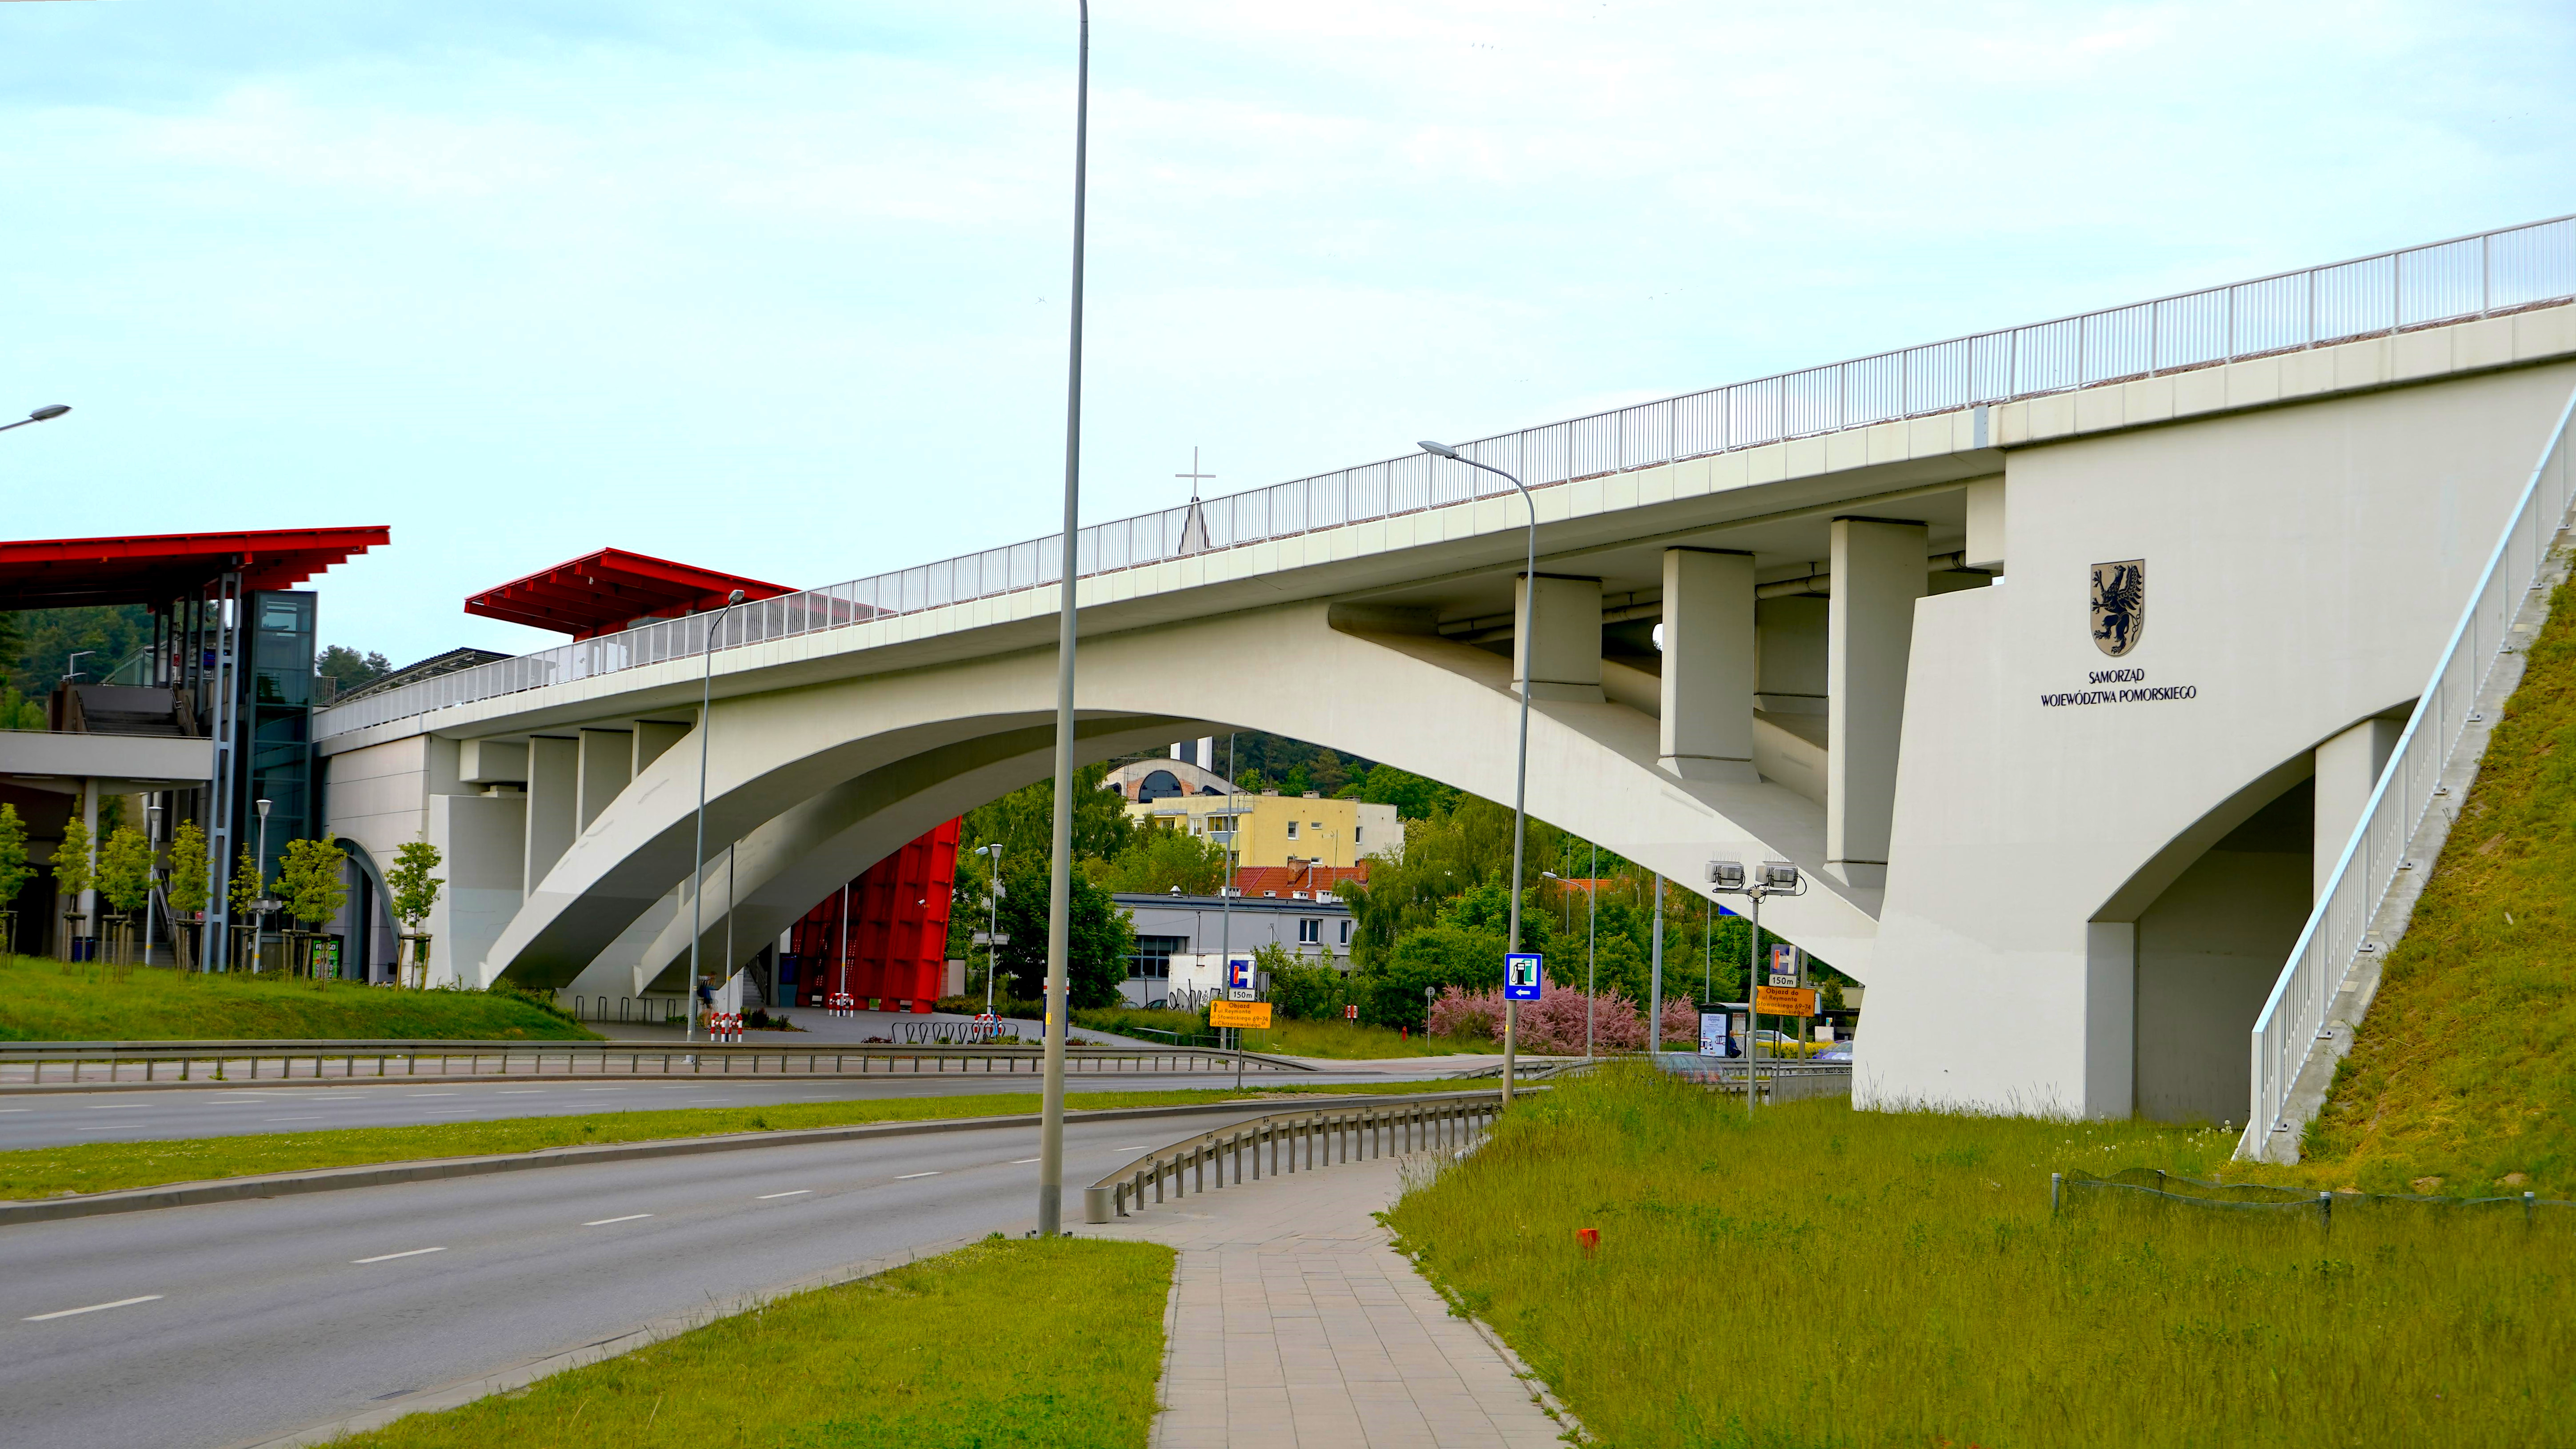
\includegraphics[width=0.48\linewidth]{/mosty_wstep/photos/kolejowy_slowackiego_1.jpg} \label{fig:arch_deck_bridges_a}} \;
%	%
%	\subfloat[Wiaduk kolejowy nad ul. Hallera w Gdańsku (arch. własne)]{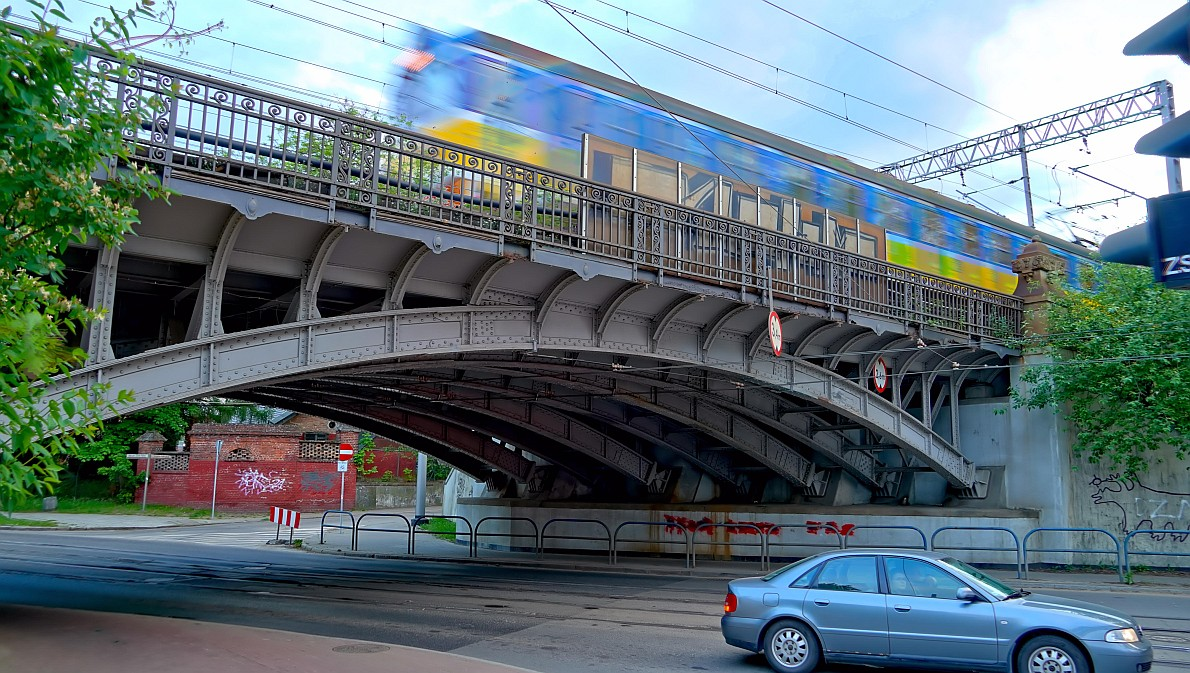
\includegraphics[width=0.48\linewidth]{/mosty_wstep/photos/kolejowy_hallera.jpg} \label{fig:arch_deck_bridges_b}} \\
%	%
%	\subfloat[Wiaduk drogowy w ciągu al. Żołnierzy Wyklętych w Gdańsku (arch. własne)]{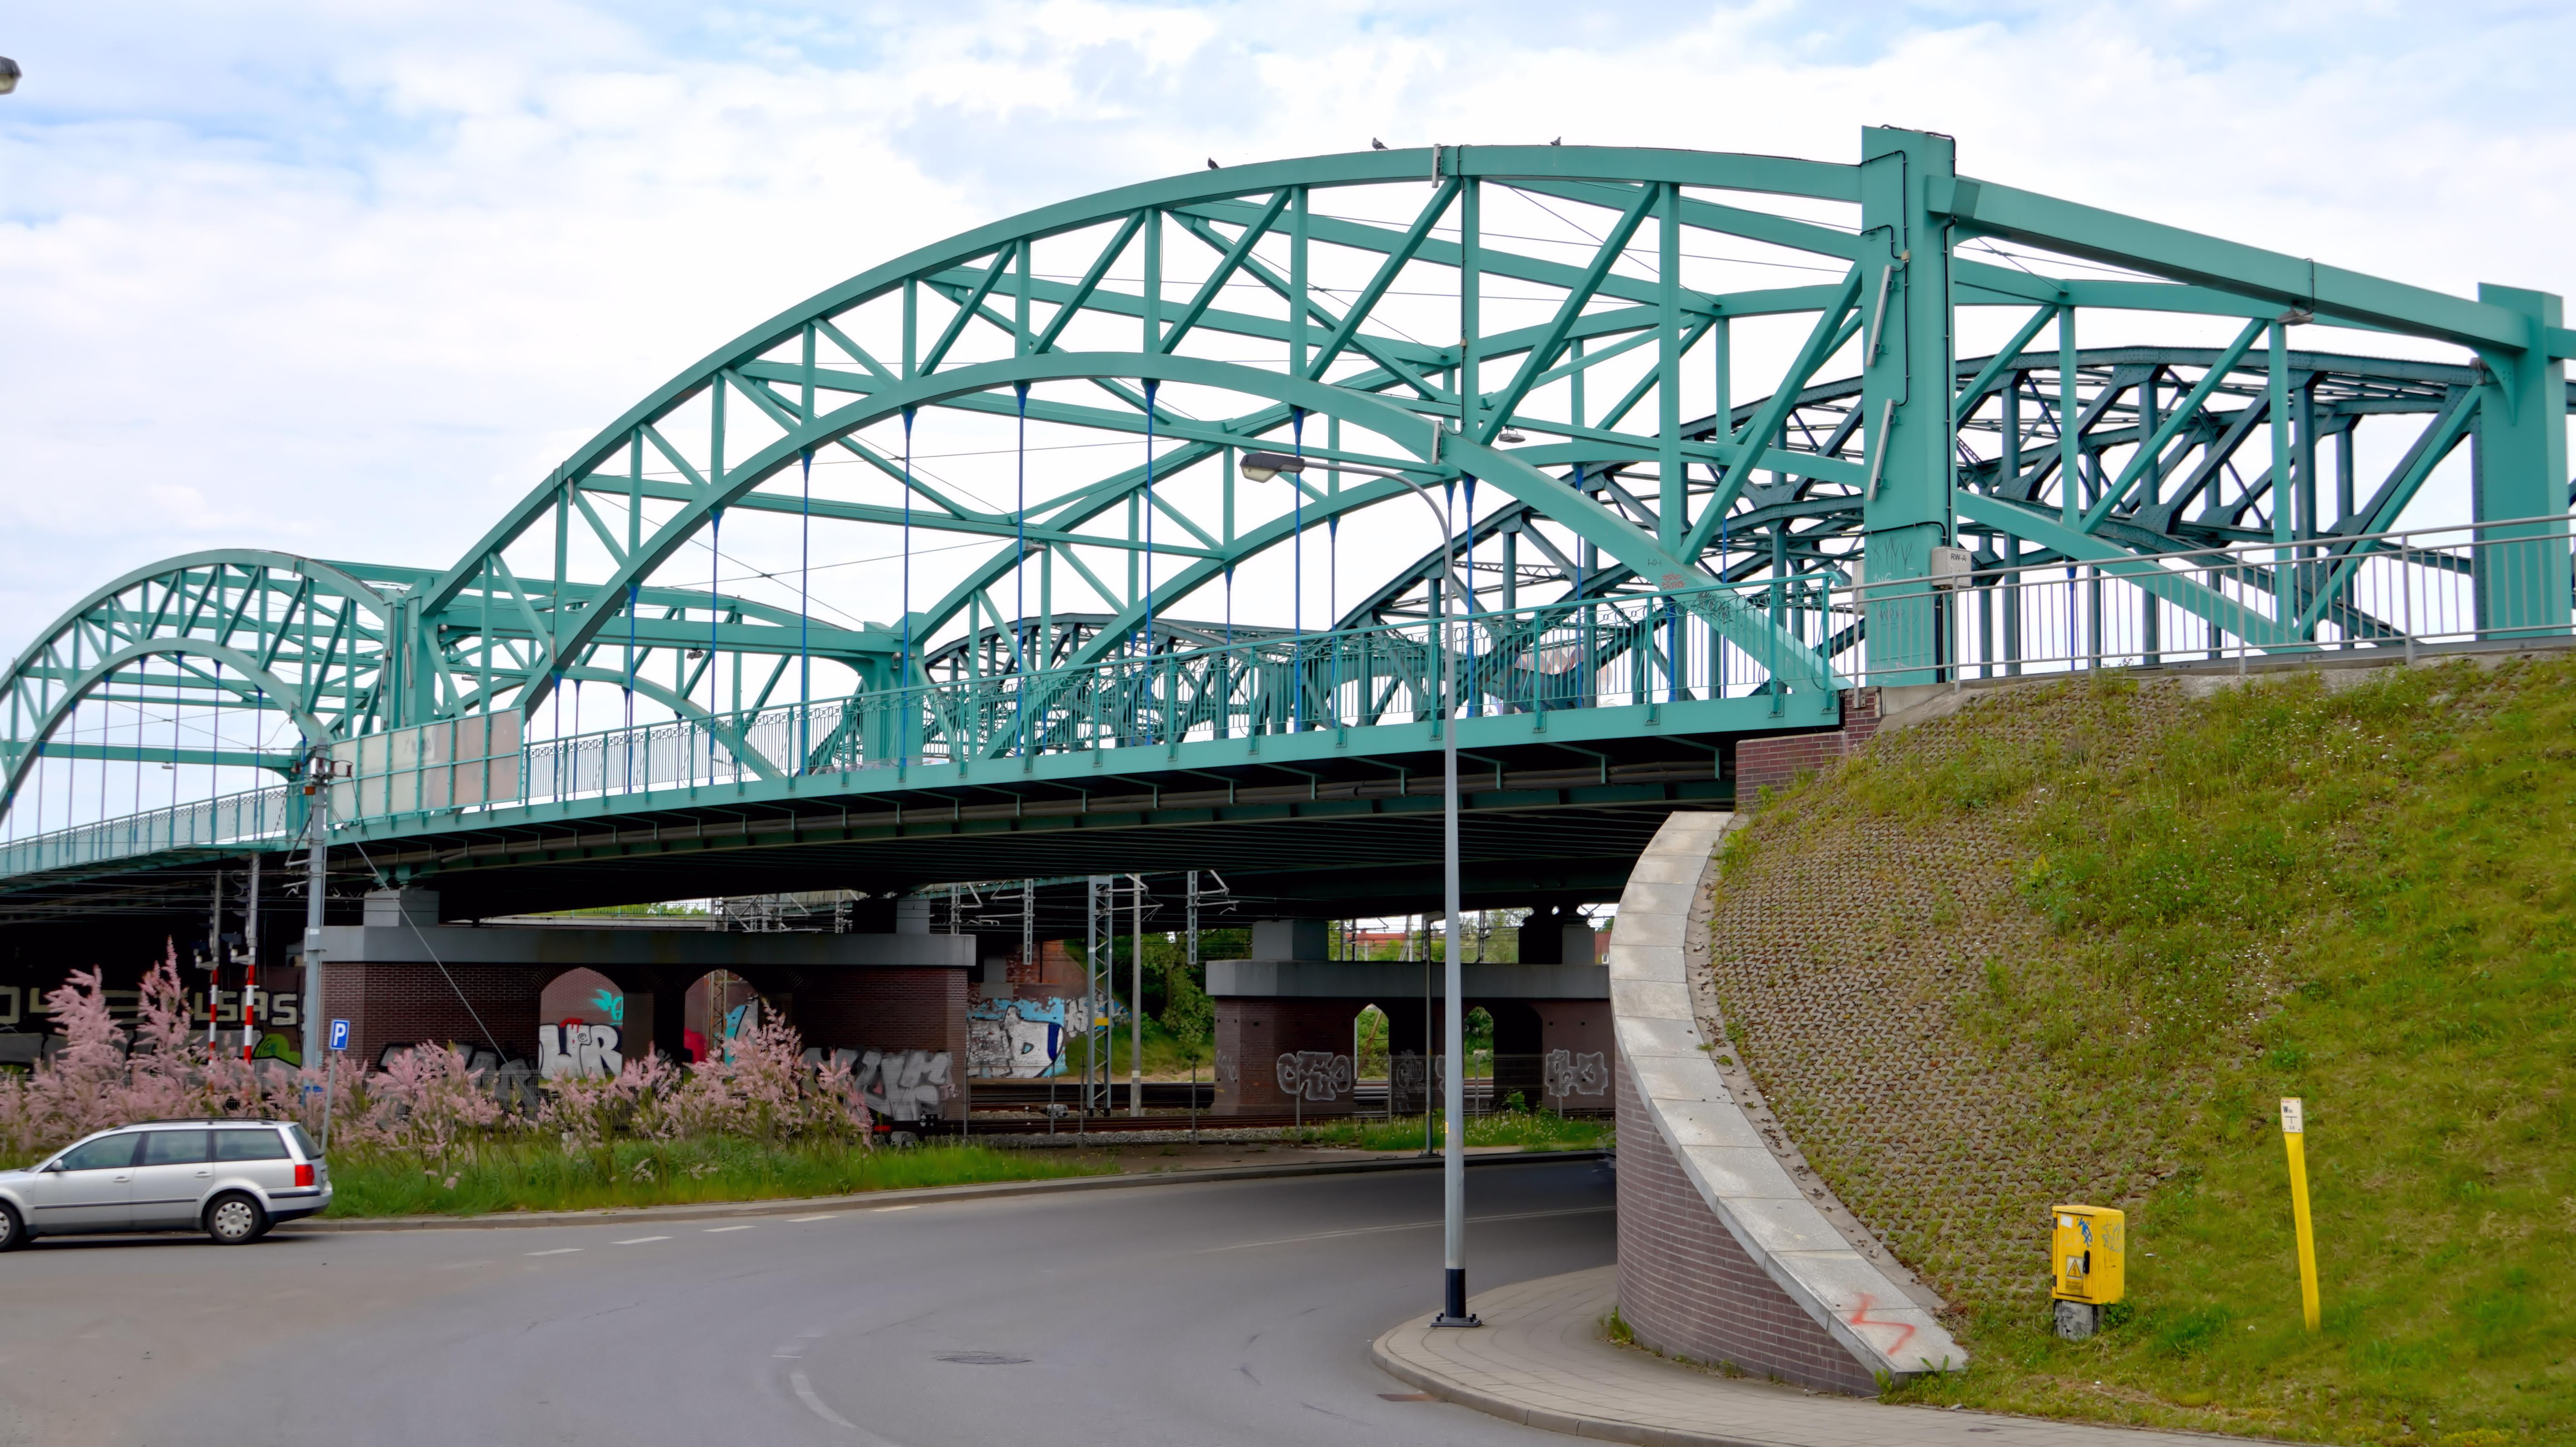
\includegraphics[width=0.48\linewidth]{/mosty_wstep/photos/lukowy_kolo_GB.jpg} \label{fig:arch_deck_bridges_c}} \;
%	%
%	\subfloat[Most kolejowy przez Martwą Wisłę w Gdańsku (arch. własne)]{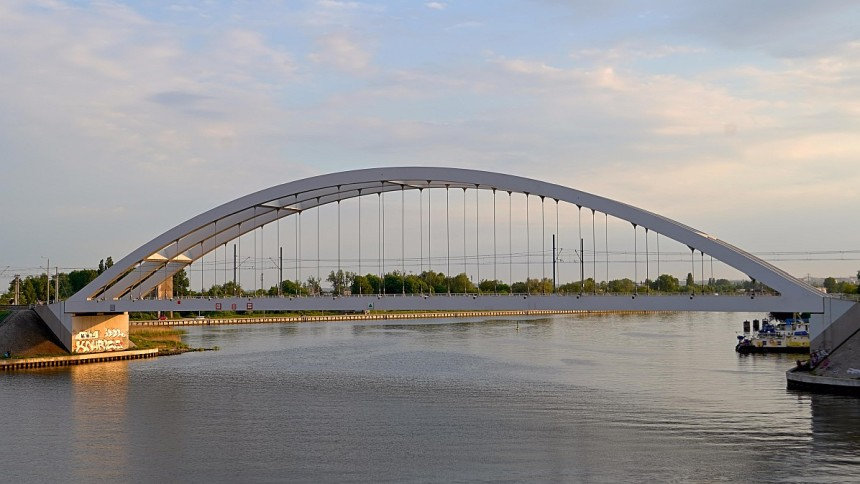
\includegraphics[width=0.48\linewidth]{/mosty_wstep/photos/kolejowy_martwa_wisla.jpg} \label{fig:arch_deck_bridges_d}} \\
%	%
%	\subfloat[Kładka dla pieszych przez Obwodnicę Trójmiasta (arch. własne)]{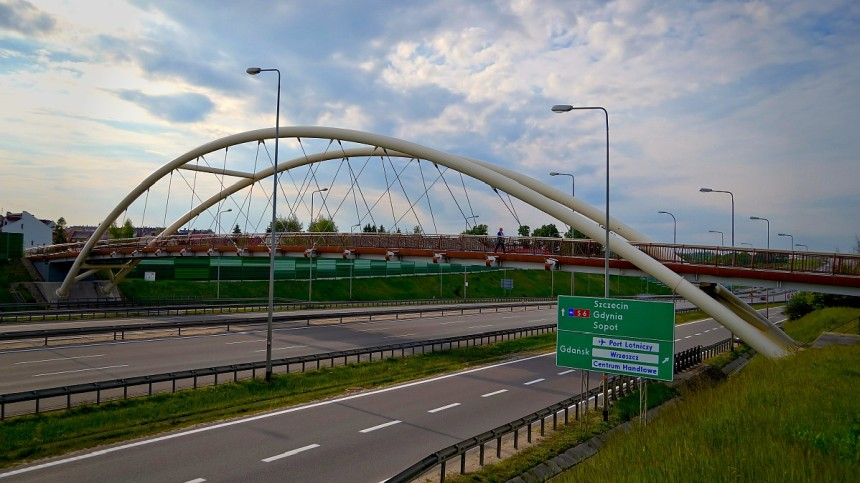
\includegraphics[width=0.48\linewidth]{/mosty_wstep/photos/kladka_obwodnica_1.jpg} \label{fig:arch_deck_bridges_e}} \;
%	%
%	\subfloat[Wiadukt drogowy w ciągu ul. Armii Krajowej w Bydgoszczy (arch. własne)]{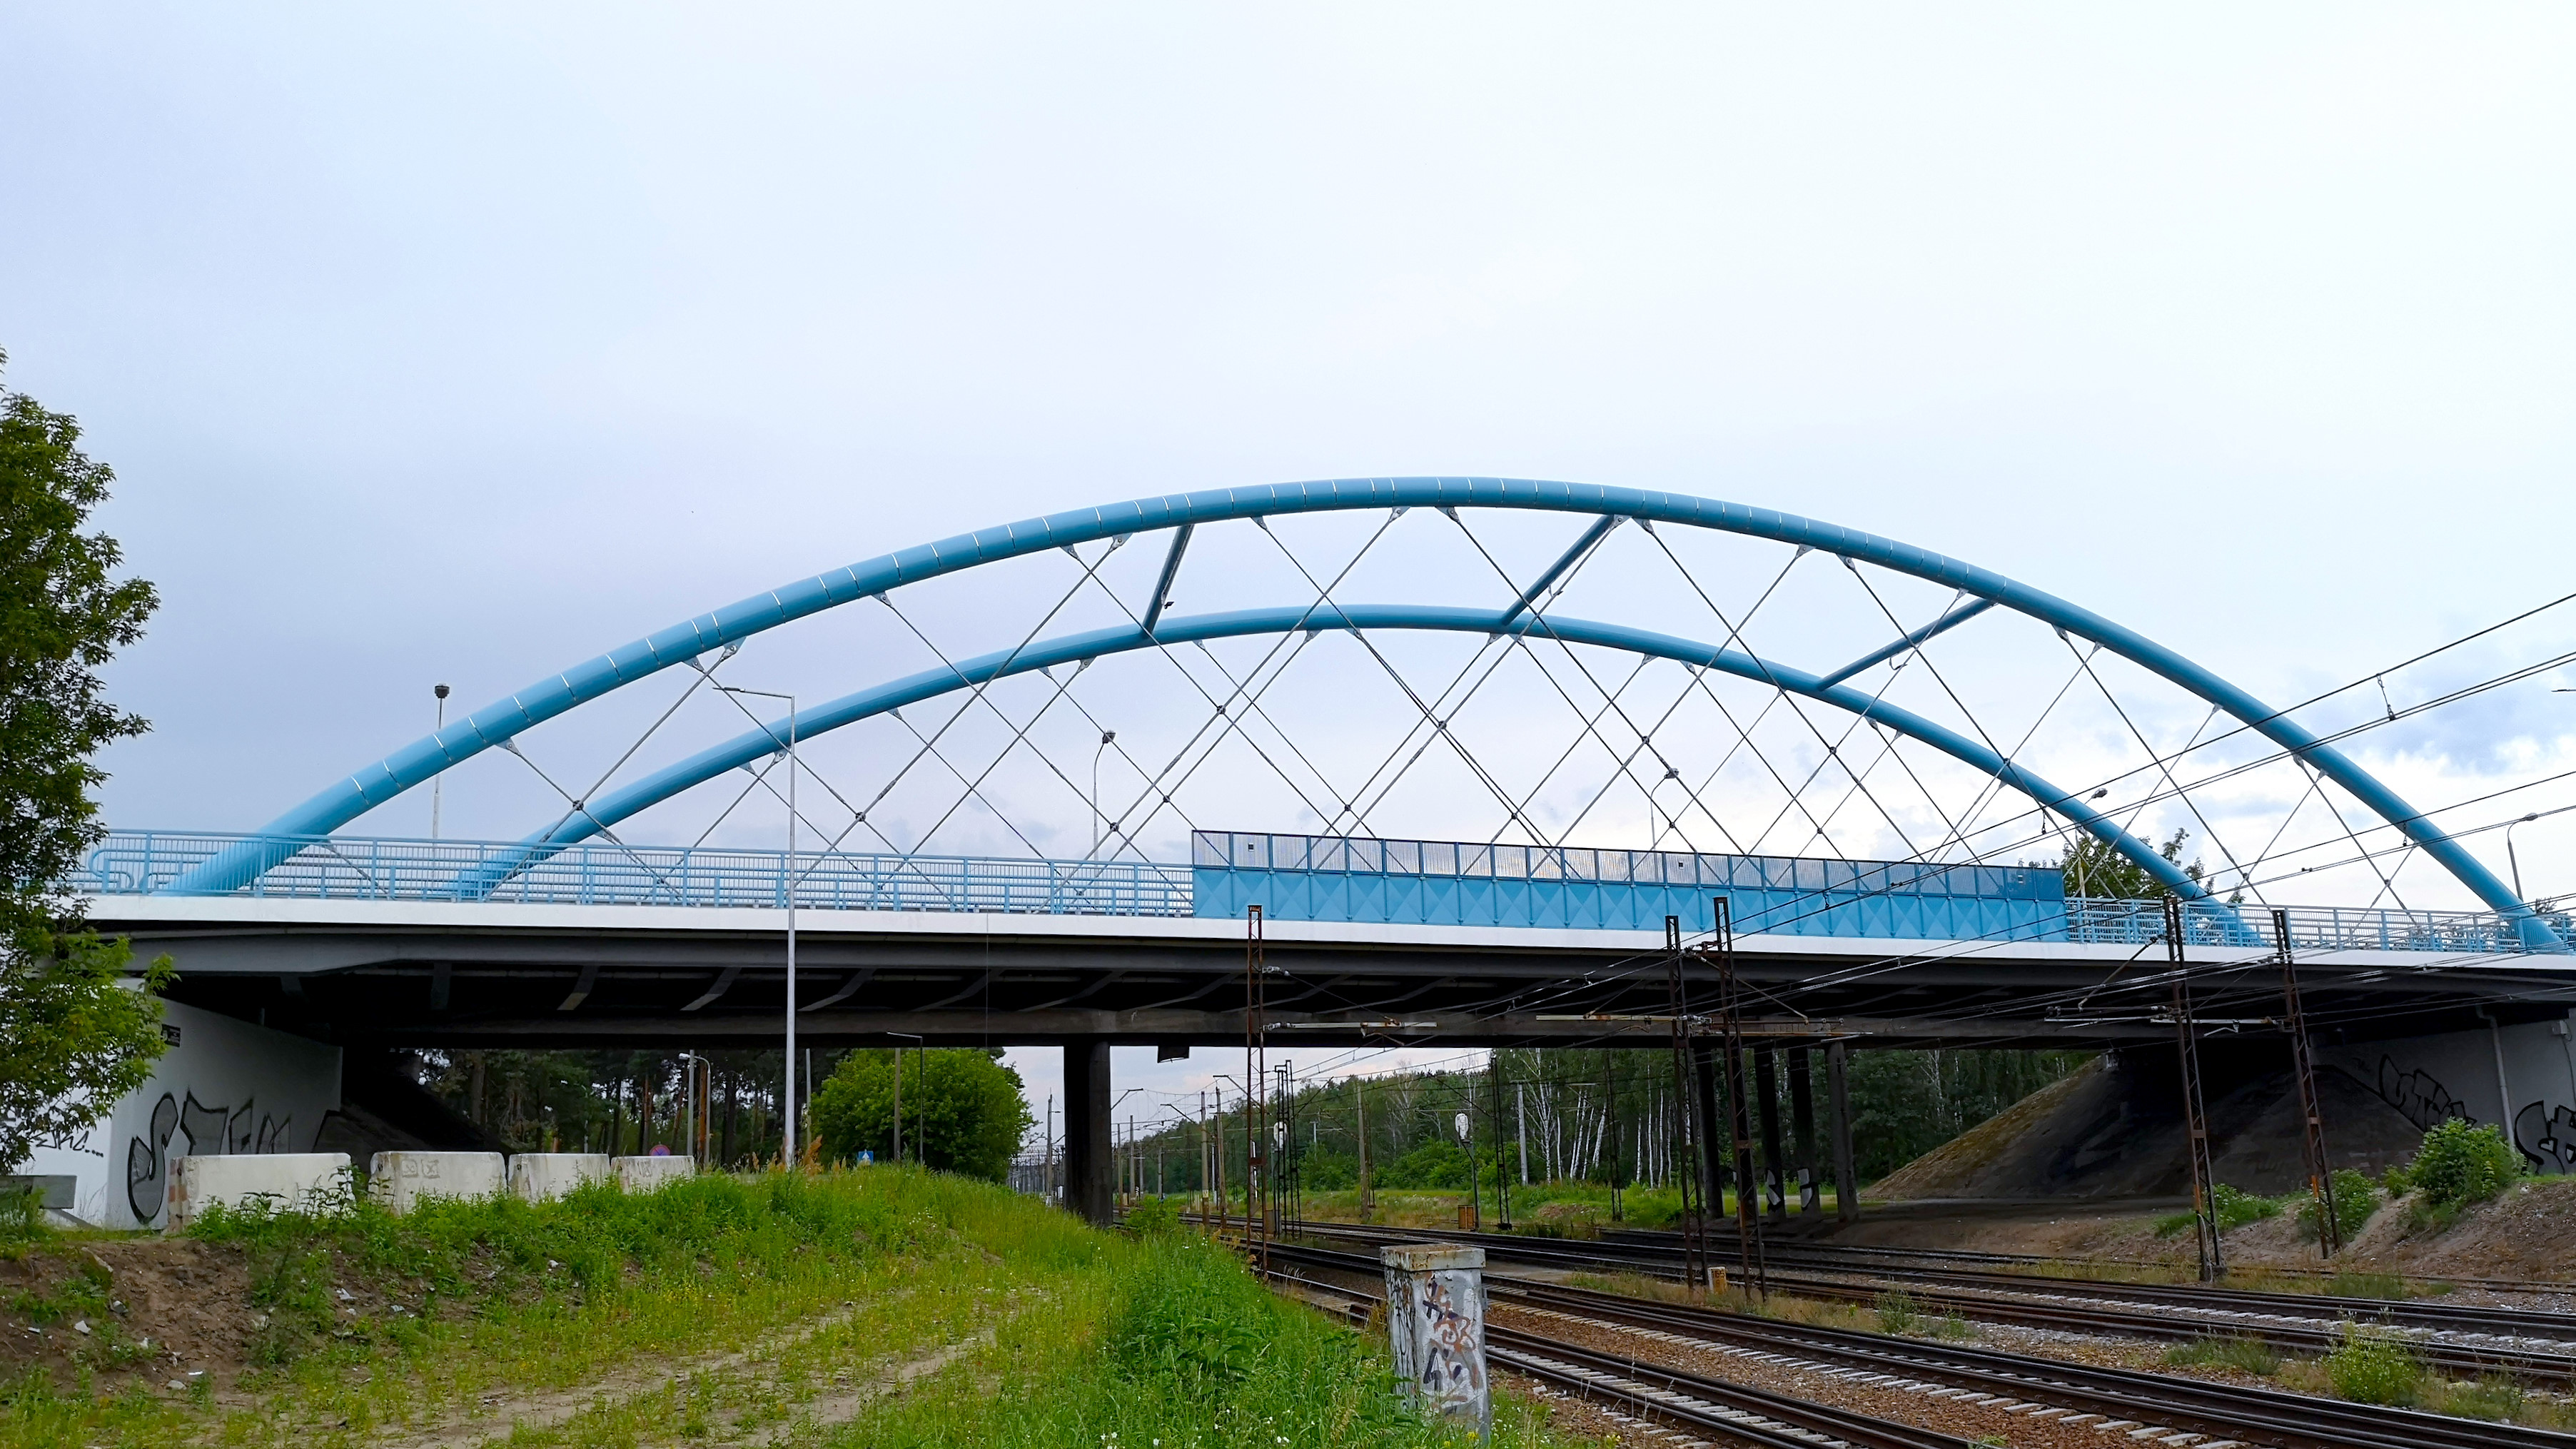
\includegraphics[width=0.48\linewidth]{/mosty_wstep/photos/wiadukt_bydgoszcz.jpg} \label{fig:arch_deck_bridges_f}} \\
%	%
%	\subfloat[Wiadukt w ciągu Obwodnicy Południowej - Gdańsk Południe (arch. własne)]{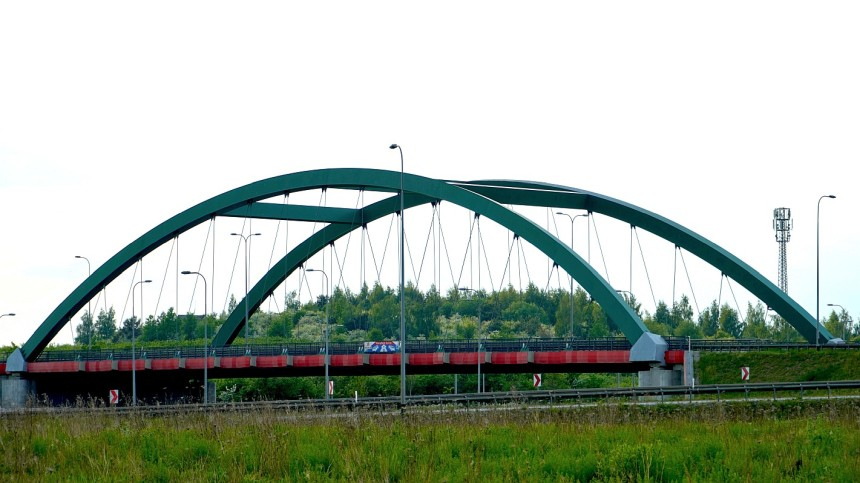
\includegraphics[width=0.48\linewidth]{/mosty_wstep/photos/kolejowy_POG_1_1.jpg} \label{fig:arch_deck_bridges_g}} \;
%	%
%	\subfloat[Wiadukt WD0 nad Obwodnicą Wałcza w trakcie próbnego obciążenia (arch. własne)]{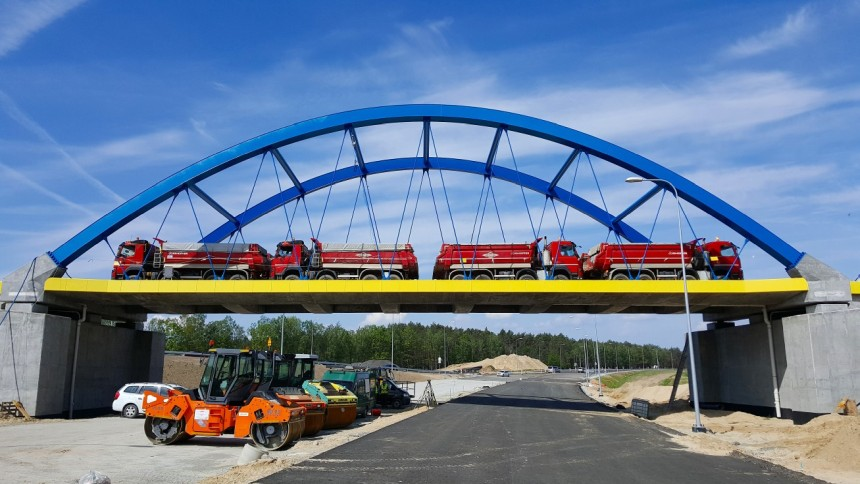
\includegraphics[width=0.48\linewidth]{/mosty_wstep/photos/probne_walcz_1.jpg} \label{fig:arch_deck_bridges_h}}
%	%
%	\caption{Wybrane polskie mosty łukowe: (a) wiadukt z jazdą górą i dźwigarem żelbetowym, (b) wiadukt z jadą górą i dźwigarem stalowym, (c) wiadukt z jazdą dołem i dźwigarem kratowym, (d) most z jazdą dołem i dźwigarem stalowym, (e) kładka dla pieszych z wieszakami typu Network, (f) wiadukt z wieszkami typu Network, (g) wiadukt z wieszkami Nielsena, (h) wiadukt z wieszkami Nielsena w trakcie próbnego obciążenia}
%	\label{fig:arch_deck_bridges}
%\end{figure}

Mosty z jazdą górą budowane są kiedy pod obiektem jest na tyle dużo miejsca, że możliwe jest zastosowanie dużej wysokości konstrukcyjnej. Taka sytuacja ma miejsce na przykład w terenach górzystych. W przeciwnym przypadku gdy wymagana jest mała wysokość konstrukcyjna uzasadnione jest stosowanie obiektów o jeździe dołem lub pośredniej. 

Obciążona konstrukcja łukowa z zasady generuje siły poziome na podłoże. Nazywa się je reakcjami rozporowymi lub po prostu rozporem. W przypadku obiektów z jazdą dołem lub jazdą pośrednią możliwe jest wyeliminowanie reakcji poziomych przez zastosowanie ściągu. Rolę ściągu może stanowić odrębny element konstrukcyjny jak również cały pomost. Wykorzystanie pomostu jest obecnie bardzo częstym rozwiązaniem. Dotyczy to zarówno pomostów stalowych jak i betonowych. W przypadku pomostów betonowych stosuje się sprężenie niwelujące efekt rozciągania pochodzącego od rozporu.

Mosty łukowe wykonywane są obecnie z dwóch materiałów: stali i betonu (w tym betonu sprężonego). Zależnie od materiału dźwigar łukowy może posiadać różną strukturę. Najczęściej łuki występują w następujących formach \parencite{Cholewo1965}:
\begin{itemize}
	\item pełnościenny przekrój łuku (dźwigar stalowy) (Rys. \ref{fig:arch_deck_bridges_b}),
	\item łuk w postaci kratownicy (dźwigar stalowy) (Rys. \ref{fig:arch_deck_bridges_c}),
	\item pełny przekrój lub w postaci skrzynki (dźwigar betonowy) (Rys. \ref{fig:arch_deck_bridges_a}),
	\item zespolony przekrój ze stalowym płaszczem wypełnionym betonem \teng{CFST - Concrete Filled Steel Tubes} \parencite{Abramski2019}.
\end{itemize}

W przeważającej większości mosty łukowe projektowane są obecnie jako konstrukcje statycznie niewyznaczalne. Z tego względu mogą one różnić się mechanizmem pracy również w zależności od sztywności poszczególnych elementów konstrukcyjnych. Kiedy zarówno łuk jak i dźwigar pomostu odpowiadają za przeniesienie sił normalnych i momentów zginających mamy do czynienia z układem Lohse'a. Przypadek ten wystąpi kiedy łuk i ściąg posiadają znaczącą sztywność giętną. Odmienna sytuacja występuję w przypadku układu Langera, kiedy to wiotki dźwigar łukowy \textit{de facto} jedynie usztywnia dźwigar belkowy. W tej sytuacji łuk przenosi teoretycznie jedynie siły osiowe \parencite{Lin2017}. 

Standardowe rozpiętości dla przęseł łukowych kształtują się w zakresie od 40 do około 400 w przypadku mostów betonowych i do 500 m w przypadku mostów stalowych \parencite{Madaj2009}. \cite{Czudek1997} przedstawił dla mostów stalowych statystykę uwzględniającą typowe rozpiętości w zależności od rodzaju przęsła łukowego. Dla tradycyjnych przęseł łukowych podał zakres od 40 do 300 m, dla łuków typu Langera od 40 do 150 m, dla łuków typu Lohse'a od 60 do 200 m, a dla łuków Nielsena i Network (Rys. \ref{fig:bridges_types_hangers}) od 110 do 200 m. Aktualnie na światowej liście mostów łukowych o największej rozpiętości pierwsze miejsce zajmuje chiński most \textit{Pingnan Third Bridge} (Rys. \ref{fig:arch_bridges_a} \parencite{Contributors2021,Biliszczuk2015a}. Został on oddany do użytku 28 grudnia 2020 roku, a jego rozpiętość wynosi 575 m. Warto wspomnieć, że na liście obiektów o rozpiętości powyżej 300 m znajduje się obecnie 76 pozycji z czego zdecydowaną większość (47 pozycji) stanowią mosty chińskie, a drugą pozycję pod względem liczebności zajmują Stany Zjednoczone Ameryki z 9 obiektami. Pod względem wykorzystanych materiałów większość dźwigarów łukowych jest wykonana ze stali (44 pozycje). Pozostałe obiekty  zbudowane są z elementów CFST (19 pozycji) i betonu (13 pozycji). Najstarszy na liście obiekt \textit{Bayonne Bridge} został oddany do użytku w 1931 roku i wciąż zajmuje wysoką, szóstą pozycję na liście z rozpiętością 510 m (Rys. \ref{fig:arch_bridges_b}). W Polsce rekordowe przęsło łukowe stanowi most im. gen. Elżbiety Zawackiej w Toruniu (Rys. \ref{fig:arch_bridges_c}). Jest to most drogowy przez Wisłę, złożony z dwóch głównych przęseł łukowych o rozpiętości 270 m każde \parencite{Wachalski2015}. Obszerne omówienie historii mostów łukowych na ziemiach polskich przedstawił \cite{Biliszczuk2015}.
 
\begin{figure}[bt!]
	\centering
	\captionsetup{justification=centering}
	\subfloat[Pingnan Bridge\\(fot. Xinhua/Cao Yiming)]{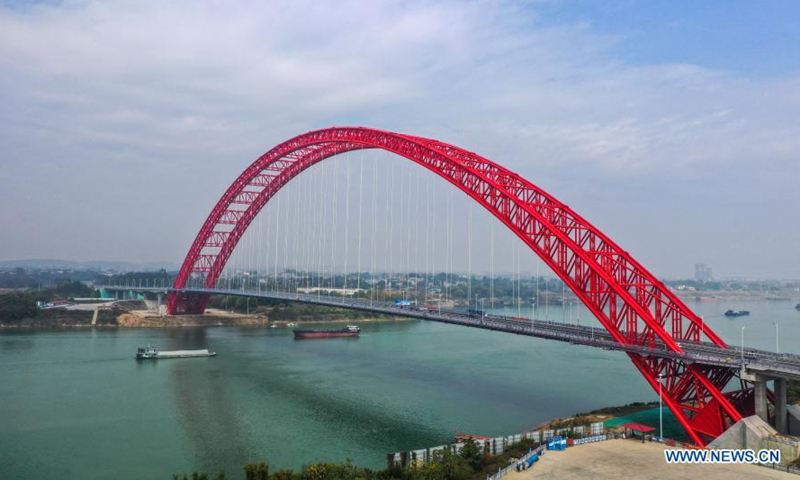
\includegraphics[height = 3.5cm]{/mosty_wstep/photos/pingnan_third_bridge.jpeg} \label{fig:arch_bridges_a}}\;
	\subfloat[Bayonne Bridge\\(fot. Jim Henderson)]{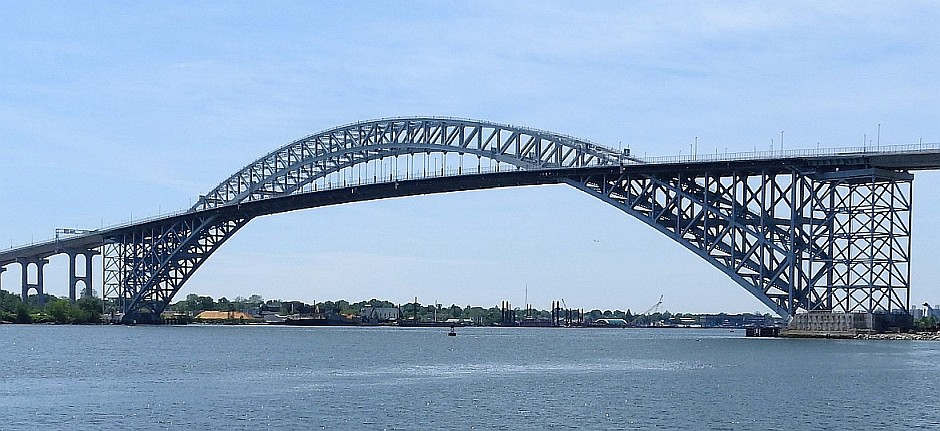
\includegraphics[height = 3.5cm]{/mosty_wstep/photos/High_BB_from_Bayonne_jeh_croped.jpg} \label{fig:arch_bridges_b}}\\
	\subfloat[Most im. gen. Elżbiety Zawackiej\\(fot. Wikipedia User: Pko)]{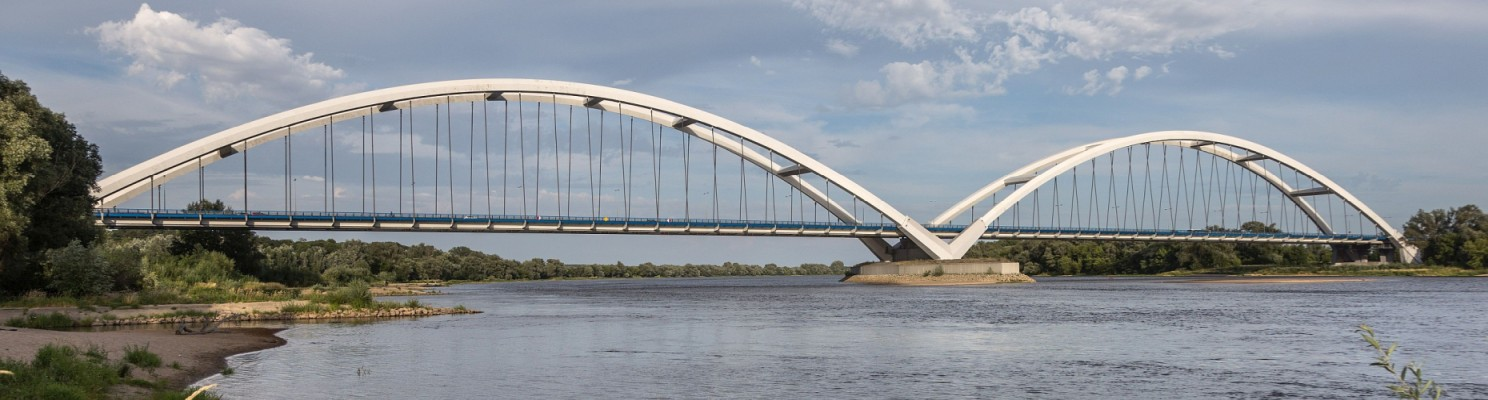
\includegraphics[width = 13.7cm]{/mosty_wstep/photos/Torun_most_Zawackiej_croped.jpg} \label{fig:arch_bridges_c}} \\

	
	\caption{Rekordowe mosty łukowe świata i Polski}
	\label{fig:arch_bridges}
\end{figure}





\subsubsection{Połączenie pomostu i dźwigara łukowego}
Połączenie pomiędzy pomostem, a dźwigarem łukowym realizuje się za pomocą ścian lub słupków kiedy pomost znajduje się ponad dźwigarem. Kiedy pomost należy podwiesić do dźwigara stosowane są wieszaki. Tradycyjnie łączniki w obu wariantach są ukształtowane jako pionowe. Liczba łączników przyjmowana jest zwykle jako parzysta, tak by klucz łuku znajdował się pośrodku odstępu między wieszakami \parencite{Szczygie1978}. W przypadku konstrukcji z jazdą górą odstępstwa od pionowego ukształtowania słupków zastosował między innymi Morandi (Rys. \ref{fig:bridges_morandi}). 

\begin{figure}[hbt!]
	\centering
	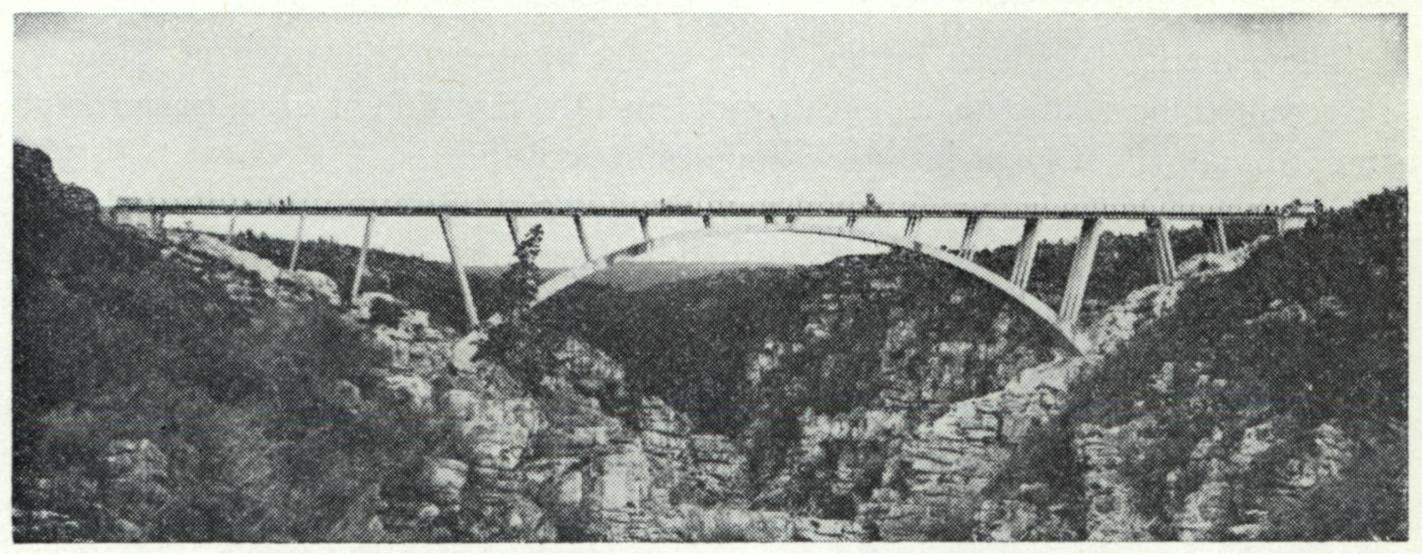
\includegraphics[]{/mosty_wstep/photos/Morandi-works.jpg}
	\captionsetup{justification=centering}
	\caption{\textit{Paul Sauer Bridge} - most betonowy z jazdą gorą i słupkami ukośnymi. Projektant: Riccardo Morandi \parencite{Morandi1962}}
	\label{fig:bridges_morandi}
\end{figure}

W przypadku obiektów z jazdą dołem występują trzy główne schematy rozkładu wieszaków:
\begin{itemize}[noitemsep]
	\item wieszaki proste (Rys. \ref{fig:bridges_types_hangers_a}, \ref{fig:arch_deck_bridges_c}, \ref{fig:arch_deck_bridges_d}),
	\item wieszaki ukośne - Nielsena (Rys. \ref{fig:bridges_types_hangers_b}, \ref{fig:arch_deck_bridges_g},  \ref{fig:arch_deck_bridges_h}),
	\item wieszaki typu Network (Rys. \ref{fig:bridges_types_hangers_c}, \ref{fig:arch_deck_bridges_e}, \ref{fig:arch_deck_bridges_f}).
\end{itemize}

\begin{figure}[h]
	\centering
	\subfloat[wieszki proste]{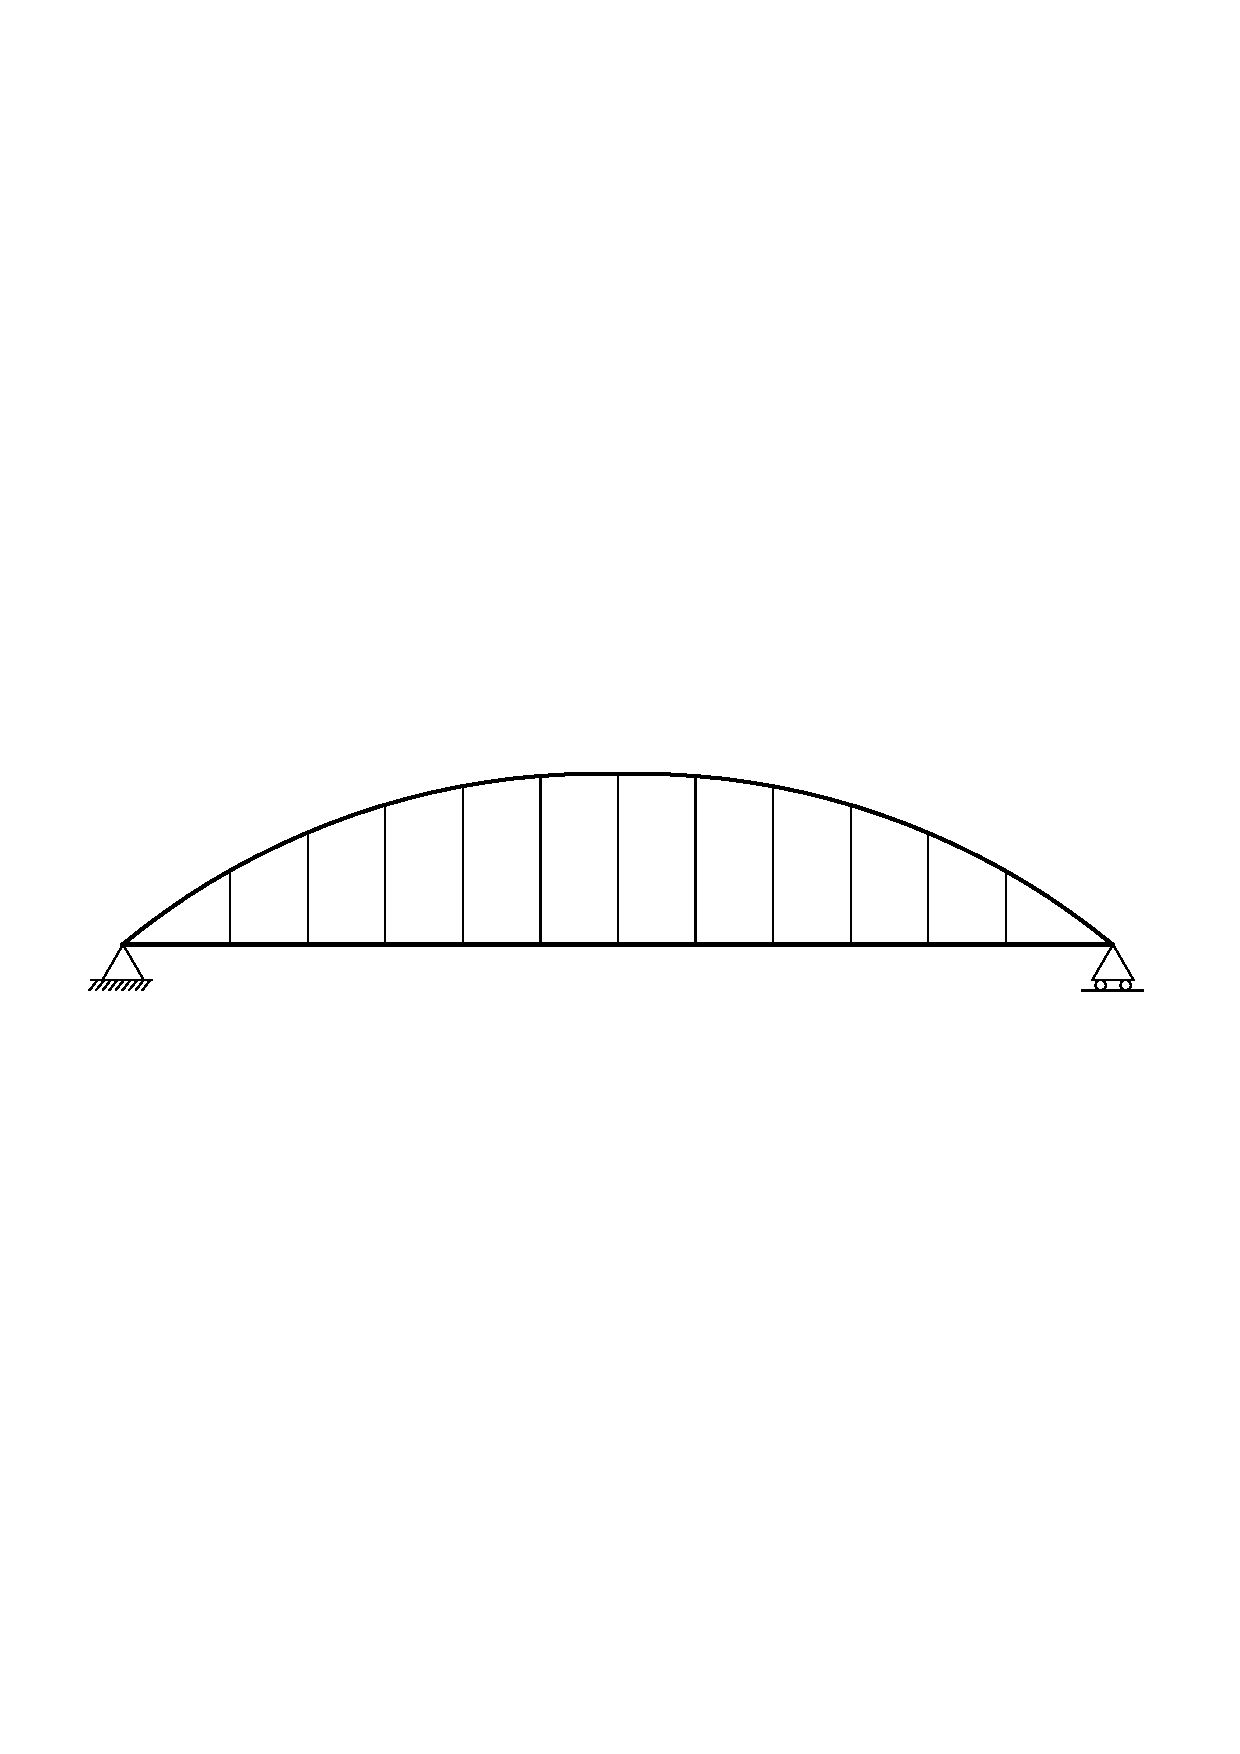
\includegraphics[width=0.7\linewidth,page=1]{/mosty_wstep/mosty.pdf} \label{fig:bridges_types_hangers_a}}  \\
	\subfloat[wieszaki ukośne]{\includegraphics[width=0.7\linewidth,page=2]{/mosty_wstep/mosty.pdf} \label{fig:bridges_types_hangers_b}} \\
	\subfloat[wieszaki typu Network]{\includegraphics[width=0.7\linewidth,page=3]{/mosty_wstep/mosty.pdf} \label{fig:bridges_types_hangers_c}}
	\captionsetup{justification=centering}
	\caption{Układy statyczne mostów łukowych ze ściągiem różniących się układem wieszaków}
	\label{fig:bridges_types_hangers}
\end{figure}

Wieszaki proste są tradycyjnym rozwiązaniem. Względem pozostałych typów charakteryzują się przede wszystkich prostotą wykonania i znacznie mniejszą sztywnością globalną przęsła. System wieszaków ukośnych został zaproponowany przez Octaviusa F. Nielsena w roku 1926. Przyczynkiem do opracowania tego rozwiązania było zjawisko wyłączania się niektórych wieszaków prostych przy obciążeniu ruchomym. W systemie Nielsena nie przewidziano przecinania się wieszaków, a jedynie nachylenie ich pod kątem. Ewolucję tego rozwiązania zaproponował w roku 1955 Per Tveit w swojej pracy magisterskiej. W tym wariancie niektóre z wieszaków przecinają się przynajmniej dwukrotnie \parencite{Tveit2019}. W Polsce funkcjonuje angielska nazwa tego sytemu \textit{Network}. \cite{Tveit2019} podał największą zaletę korzystania z wieszaków typu Network: zapewniają najmniejszą smukłość i lekkość konstrukcji spośród wszystkich wariantów konstrukcji łukowych. Wynika to z większej - w porównaniu do innych systemów - sztywności globalnej konstrukcji, a w konsekwencji powstają mniejsze ugięcia w przęśle i mniejsze obroty na podporach.

W warunkach idealnych podstawowym schematem pracy wieszaka jest osiowe rozciąganie. W rzeczywistości istnieją jednak również inne obciążenia działające na wieszaki, zaburzające stan osiowego rozciągania. Sa to przede wszystkim \parencite{Zobel2015}:
\begin{itemize}[noitemsep]
	\item obciążenie poprzeczne od ciężaru własnego (system Nielsena i Network),
	\item obciążenie wiatrem,
	\item wpływ imperfekcji montażowych,
	\item nierownomierne ogrzanie,
	\item obciążenie oblodzeniem,
	\item wzbudzenia dynamiczne od drgań konstrukcji i zmian ciśnienia powietrza podczas przejazdu,
	\item ryzyko wyboczenia przy ściskaniu.
\end{itemize}

Elementem strukturalnym, który predestynowany jest do pracy w stanie osiowego rozciągania jest cięgno. Pomimo, że schemat statyczny konstrukcji łukowej najczęściej zakłada przegubowe połączenie pomiędzy wieszakami i dźwigarem w rzeczywistości stosowane są rozwiązania mniej lub bardziej spełniające to założenie. Dwie skrajności stanowią wieszaki sztywno i przegubowo połączone z dźwigarem. 


Sztywne połączenie może wystąpić dla wieszaków posiadających istotną sztywność giętną lub na tyle wiotkich, że sztywność giętna jest pomijalna. Pierwsze wykonywane są z profili pełnościennych stalowych lub z betonu sprężonego. W przeszłości takie rozwiązanie wykorzystywano, ponieważ niemożliwe lub nieracjonalne technologiczne było wykonanie wieszaków cięgnowych. Z taką sytuacją można spotkać się na przykład w łukowych mostach nitowanych (Rys. ) z pierwszej połowy XX w. Obecnie tego typu wieszaki wykorzystywane są kiedy konstrukcja wymaga usztywnienia poprzecznego łuku, na przykład w przypadku braku stężeń górnych. Należy pamiętać, że w takim przypadku obliczeniowo struktura odbiega w swojej pracy od schematu statycznego łuku i przybliża się do kratownicy Vierendeela. Sztywno połączone z konstrukcją mogą być również wieszaki prętowe o małej sztywności giętnej. Wykonywane są najczęściej jako spawane do blach węzłowych (Rys. \ref{}) Rozwiązanie to ma uzasadnienie przede wszystkim ekonomiczne - jest tańsze niż rozwiązania systemowe. Ze względu na złożony stan naprężeń w połączeniu należy zwrócić szczególną uwagę na zalecenia konstrukcyjne i technologiczne \parencite{Gunther2000,BundesanstaltfurWasserbauHg.2018,Szafranski2017}. 

Drugą obszerną grupę rozwiązań stanowią cięgna połączone przegubowo z konstrukcją. Elementy połączone w ten sposób z reguły są wiotkie i traktowane jako cięgna. Obecnie stosowane są następujące typy wieszaków cięgnowych:
\begin{itemize}[noitemsep]
	\item pręty okrągłe (Rys. \ref{fig:bridges_hangers_cs_a}),
	\item liny standardowe (Rys. \ref{fig:bridges_hangers_cs_b}) i zamknięte (Rys. \ref{fig:bridges_hangers_cs_c}),
	\item wiązki drutów równoległych lub splotów (Rys. \ref{fig:bridges_hangers_cs_d}), z indywidualnymi lub zbiorczymi zakotwieniami
\end{itemize}

\begin{figure}[hbt!]
	\centering
	\captionsetup{justification=centering}
	\subfloat[]{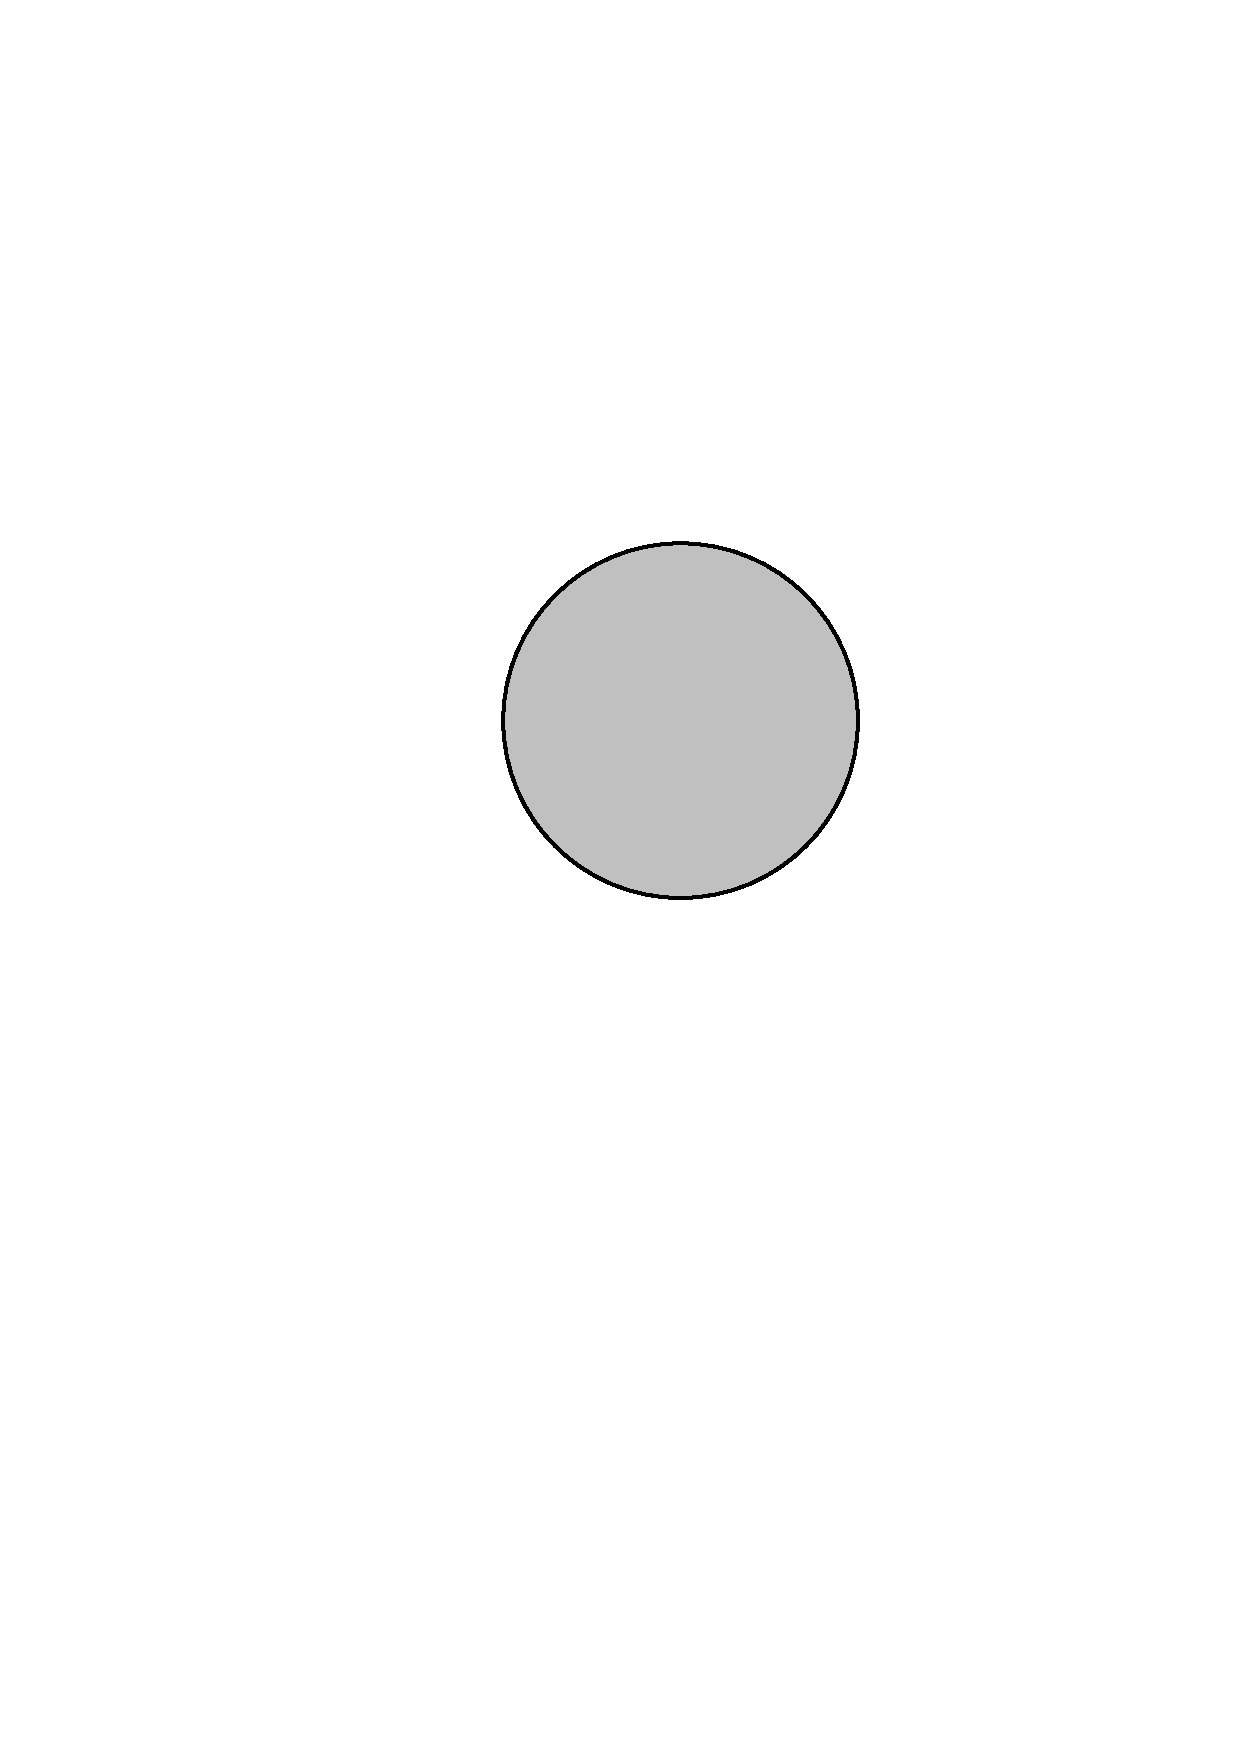
\includegraphics[height=3cm,page=1]{/mosty_wstep/wieszaki/przekroje_wieszaki.pdf} \label{fig:bridges_hangers_cs_a}} \quad
	\subfloat[]{\includegraphics[height=3cm,page=2]{/mosty_wstep/wieszaki/przekroje_wieszaki.pdf} \label{fig:bridges_hangers_cs_b}} \quad
	\subfloat[]{\includegraphics[height=3cm,page=3]{/mosty_wstep/wieszaki/przekroje_wieszaki.pdf} \label{fig:bridges_hangers_cs_c}} \quad
	\subfloat[]{\includegraphics[height=3cm,page=4]{/mosty_wstep/wieszaki/przekroje_wieszaki.pdf} \label{fig:bridges_hangers_cs_d}}	
	\caption{Przekroje poprzeczne stosowanych typów wieszaków: (a) pręty pełne, (b) lina standardowa, (c) lina o konstrukcji zamkniętej, (d) lina wielosplotowa}
	\label{fig:bridges_hangers_cs}
\end{figure}

Wieszaki cięgnowe połączone z konstrukcją przegubowo w większości wchodzą w skład prefabrykowanych systemów. Dzięki odpowiedniemu systemowi jakości wykonania i badaniom laboratoryjnym potwierdzonych aprobatami, w trakcie projektowania nie ma konieczności konstruowania i sprawdzania poszczególnych elementów połączenia przegubowego i mechanizmów regulacji. Cięgna dobiera się na podstawie katalogów w zależności od wymaganej nośności. Ma to istotne znaczenie zwłaszcza w kontekście wymogów normowych. W zakresie normy \parencite{PN-EN-1993-1-112008} dotyczącej projektowania konstrukcji cięgnowych mieszczą się wszystkie wymienione wyżej typy cięgien połączonych przegubowo. Norma przede wszystkim podaje zasady ustalania wymagań technicznych cięgien dla oceny bezpieczeństwa, użytkowalności trwałości. Zgodnie z filozofią przedstawioną w Eurokodzie 0 wyróżnia 3 stany graniczne, które muszą być spełnione przy projektowaniu:
\begin{itemize}[noitemsep]
	\item Stan Graniczny Nośności \teng{Ultimate Limit State} - porównanie siły osiowej z nośnością obliczeniową przy rozciąganiu,
	\item Stan Graniczny Użytkowania \teng{Serviceability Limit State} - ograniczenie wartości naprężeń i odkształceń,
	\item Stan Graniczny Zmęczenia \teng{Fatigue Limit State} - sprawdzenie zakresów zmienności naprężeń.
\end{itemize}
Dodatkowo w normie zapisano wymóg możliwości regulacji i wymiany cięgien. 




\section{Obliczenia konstrukcji za pomocą Metody Elementów Skończonych}
Metody analityczne wyznaczania wartości odpowiedzi czy stanu konstrukcji nie mają już wiodącego zastosowania przy rozwiązywaniu rzeczywistych problemów inżynierskich. Model matematyczny oparty na równaniach różniczkowych może być rozwiązany w postaci zamkniętej jedynie w przypadku relatywnie prostych przypadków. Wiele z rzeczywistych rzeczywistych układów charakteryzuje się skomplikowanym kształtem, niejednorodnym materiałem, bądź złożonymi warunkami brzegowymi i nie istnieją dla nich ścisłe rozwiązania. Akceptując brak ścisłych rozwiązań opracowano metody przybliżone, oparte na procesie dyskretyzacji. \cite{Rakowski2016} definiują dyskretyzacją jako proces, w którym przekształca się opis pola wyrażony za pomocą nieskończenie wielu parametrów, w opis wyrażony przez skończona liczbę wartości zlokalizowanych w skończonej liczbie punktów (węzłów). Zmienność pola pomiędzy węzłami definiują funkcje kształtu. Istnieją dwie wiodące metody budowy modelu dyskretnego: Metoda Różnic Skończonych (MRS) i Metoda Elementów Skończonych (MES), oraz mniej popularne Metoda Całkowania Numerycznego (MCN) i Metoda Elementów Brzegowych (MEB). W analizie konstrukcji MES jest metodą znacznie bardziej popularną, stosowaną w większości programów komercyjnych. W poniższej pracy przy wyznaczaniu stanu konstrukcji posłużono się komercyjnym środowiskiem MES SOFiSTiK. Literatura przedmiotu dotycząca MES jest bardzo rozbudowana. Do podstawowych pozycji opisujących rozwój należą \parencite{Kleiber1985,Hughes1987,Zienkiewicz2005,Rakowski2016}. Ze względu na obszerność tematu zaniechano przytoczenia podstaw i definicji metody,a skupiono się jedynie na jej zastosowaniu i elementach rozwijających niektóre jej aspekty. Stosowalność MES w analizie konstrukcji została wielokrotnie potwierdzona w literaturze. Autor pracy również wielokrotnie wykorzystywał MES przy rozwiązywaniu rzeczywistych problemów inżynierskich. W następujących pracach opisane niektóre z nich, w których autor brał czynny udział wykorzystując metody numerycznych analizy konstrukcji \parencite{Zotowski2016d,Zotowski2017a,Cudny2017,Zotowski2017h,Zotowski2018a,Zoto wski2018d,Zotowski2018c,Binczyk2020a}.

Pomimo długiej historii rozwoju i wielokrotnie potwierdzonej stosowalności MES w analizie konstrukcji zawsze trzeba pamiętać, że MES jest metodą numeryczną i ma charakter przybliżony. Wynika to z uproszczenia nieskończonego pola w procesie dyskretyzacji  i zastosowania funkcji interpolacyjnych. Niedoskonałość metody jest jednym ze źródeł możliwych niedokładności ostatecznego modelu obliczeniowego. Drugie kluczowe przybliżenie wynika z niedoskonałości odwzorowania modelu względem konstrukcji i dotyczy jej kształtu, materiału czy warunków brzegowych. Zagadnienie to zostało szerzej omówione w punkcie \ref{sect:calibration_model}. Istnieją różne metody ograniczenia i kontroli każdego z tych dwóch grup źródeł błędów. W przypadku stosowania elementów dostosowanych\footnote{Elementy dostosowane to takie, których funkcje kształtu spełniają wszystkie z trzech kryteriów: kryterium zgodności, kryterium ruchu sztywnego i kryterium stałych odkształceń \parencite{Rakowski2016}}.
błąd wynikający ze stosowania dyskretyzacji i funkcji interpolacyjnych można zmniejszać przez zagęszczenie siatki węzłów (h-convergence) lub poprzez zwiększenie rzędu funkcji interpolacyjnych (p-convergence) \parencite{Zienkiewicz2005}. W poniższej pracy przyjęto pierwszą z nich jako metodę badania zbieżności rozwiązania.

\subsection{Kalibracja modeli MES} \label{sect:calibration_model}
Pomimo coraz bardziej intuicyjnych i prostych w użyciu implementacji MES w oprogramowaniu komercyjnym wciąż wymagane jest od użytkownika doświadczenie i krytyczna ocena wykonywanych obliczeń. Oczywistym jest, że projektant lub badacz chciałby aby stworzony model jak najwierniej odwzorował zachowanie konstrukcji w jego obszarze zainteresowań. Istnieje jednak szereg czynników wpływających na brak zgodności pomiędzy modelem, a konstrukcją. Poza z zasady przybliżonym charakterem obliczeń numerycznych MES, istnieją błędy powstające w procesie modelowania. Można je podzielić na dwie grupy \parencite{Mottershead1993,Mottershead2011}:
\begin{itemize}
	\item błędy przy tworzeniu modelu i idealizacja rzeczywistej konstrukcji przez uproszczone modele mechaniczne,
	\item błędy w przyjęciu parametrów konstrukcji.
\end{itemize}

W przypadku analizy konstrukcji pierwsza grupa obejmuje błędy popełnione w trakcie wykonania takie jak: przyjęcie błędnego kształtu, niewłaściwych wartości obciążeń zewnętrznych, braku połączenia między elementami modelu. Z drugiej strony uwzględnia również błędy założeń teoretycznych takie jak: usztywnienie elastycznych połączeń, brak uwzględnienia wpływu pracy konstrukcji w innych kierunkach niż pionowy czy też przyjęcie liniowego modelu w przypadku silnej nieliniowości zachowania się konstrukcji. 

Druga grupa błędów związana z oszacowania parametrów modelu. Błędy w oszacowaniu rzeczywistych parametrów konstrukcji zaimplementowanych w modelu mogą skutkować bardzo dużymi różnicami między odpowiedzią konstrukcji rzeczywistej i przewidywaniami modelu. \cite{Brincker2015} zestawili możliwe niepewności w oszacowaniu parametrów modeli numerycznych i modalnych co przedstawiono w tabeli \ref{table:uncertainitesModel}). Jak widać niektórych z nich mogą wynosić od kilku do kilkudziesięciu procent. W przypadku warunków brzegowych na połączeniu z gruntem trudno wręcz postawić górną granice niepewności. 

Redukcja wpływu błędów grupy pierwszej zasadniczo polega na identyfikacji i eliminacji danego błędu. Analizując konstrukcje mostowe stosowane są zabiegi służące wykryciu nieprawidłowości takie jak badanie symetrii/antysymetrii odpowiedzi w przypadku symetrii/antysymetrii układu i obciążenia, przeprowadzenie analizy modalnej w celu wykrycia niepowiązanych elementów, a także sprawdzenie zgodności sumy reakcji z wartością przyłożonego obciążenia. 

Niepewności zawarte w drugiej grupie są naturalne, a zadaniem twórcy modelu jest po prostu jak najwierniejsze ich przyjęcie. Poprawę wartości parametrów można uzyskać na przykład na podstawie wykonanych badań wbudowanego materiału. Inna metoda polega na jak najlepszym dopasowaniu wybranych wartości odpowiedzi układu rzeczywistego do odpowiadających wartości odpowiedzi modelu. Zestaw procesów prowadzących do tego dopasowania nazywa się kalibracją modelu numerycznego. 

Metody kalibracji opierają się głównie na modyfikacji parametrów modelu \teng{model updating}. \cite{Batou2019} podzielił metody kalibracji na bezpośrednie - modyfikujące macierz sztywności lub mas - i pośrednie - modyfikujące parametry geometryczne, materiałowe i warunki brzegowe. Za zmianę parametrów mogą odpowiadać algorytmy o różnym stopniu skomplikowania. Najbardziej podstawowym jest modyfikacja parametrów metodą prób i błędów. Wyboru zmianianych parametrów dokonuje inżynier na podstawie doświadczenia. Jest ona skuteczna w przypadku układów niewielu parametrach i dużym doświadczeniu inżyniera. Kiedy liczba parametrów jest duża, po pierwsze ich liczba jest ograniczana na podstawie analizy wrażliwości \parencite{Friswell2001,Mottershead2011,Petersen2017,Batou2019}. Po drugie kiedy ich liczba wciąż pozostaje znacząca wykorzystywane są metody podziału na mniejsze podproblemy \parencite{Weng2020,Yu2016} bądź stosowane są metody optymalizacji globalnej takie jak metoda przeszukiwania czy też algorytmy metaheurystyczne: algorytm genetyczny czy optymalizacja rojem cząstek \parencite{Boulkaibet2015,Tran-Ngoc2018,Dan2015,Qin2018}. W pracy do kalibracji wykorzystano ostatnią z przedstawionych metod. Informacje na jej temat przedstawiono w rozdziale \ref{sect:PSO_chapter}.

Warto zwrócić uwagę, że kalibracja modelu za pomocą zmiany parametrów, przy jednoczesnym występowaniu błędów z grupy pierwszej, może prowadzić do doboru wartości parametrów o zupełnie nierealnych wielkościach. Stąd przed przystąpieniem do kalibracji modelu należy najpierw w miarę możliwości wyeliminować wszystkie błędy związane z tworzeniem modelu i jego idealizacją.

Kalibracja modelu jest wykorzystywana w wielu rzeczywistych zastosowaniach. Podstawowym celem jest maksymalne dopasowanie modelu do konstrukcji rzeczywistej w trakcie badań naukowych \parencite{Li2020,Brownjohn2001,Zhang2019,Petersen2017}. Proces ten zwany walidacją sprawia, że model numeryczny lepiej odzwierciedla rzeczywistość, a uzyskane z niego rezultaty zyskują na wiarygodności. Kalibracja służy również do oceny stanu konstrukcji i jej zmian, często w połączeniu z systemem monitoringu \parencite{Brownjohn2000,Brownjohn2003,Zoltowski2020}.

\begin{table}[hbt!]
	
	\centering
	\caption{Niepewności najistotniejszych parametrów modeli numerycznych i modalnych na podstawie \cite{Brincker2015}}
	\rowcolors{1}{}{gray!10}
	\resizebox{\textwidth}{!}{%
		\begin{tabular}{p{0.7\linewidth} | c}
			\toprule 
			Własność fizyczna   & Poziom niepewności [\%] \\
			\midrule
			Moduł sprężystości i gęstość masy dla stali i innych metali  &    1--5    \\
			Moduł sprężystości i gęstość masy dla betonu, drewna i zbrojonych włóknami materiałów & 5--20\\
			Warunki brzegowe z podłożem &    10-nieskończoność     \\
			Połączenia śrubowe & 10-nieskończoność\\
			Połączenia spawane & 2-10\\
			Masa całkowita & 1-5 \\
			Określana częstotliwość drgań własnych & 0.1-0.05\\
			Pomierzona odpowiedź & 0.2-2\\
			Określane postaci drgań własnych & 2-5\\ 
			Określane tłumienie & 5-20\\
			Współczynnik skalujący postaci drgań własnych & 5-30\\
			\bottomrule
	\end{tabular}}
	\label{table:uncertainitesModel}
\end{table}





\section{Dynamiczne obciążenie kolejowe}
Ryzyko nadmiernych drgań mostów kolejowych jest rozpatrywane od samych początków budowy dróg szynowych w Anglii na początku XIX w \parencite{Ladislav1996}. Historię tę zwięźle przedstawił w swojej pracy \cite{Szafranski2013}, opierając się na obszernych studiach literatury. Podsumowując doświadczenia naukowców i inżynierów, poza wyjątkowymi przypadkami wykolejeń i uderzeń pociągów w elementy konstrukcyjne, wywołanie niebezpiecznych amplitud drgań mostów związane jest głównie ze zjawiskiem rezonansu. Rezonans mechaniczny może wystąpić w przypadku kiedy pojawia się obciążenie cykliczne, którego częstotliwość oddziaływania pokrywa się z częstotliwością drgań własnych konstrukcji mostu. Kiedy obciążenie jest długotrwałe i w układzie nie ma tłumienia amplitudy drgań mogą teoretycznie rosnąć w nieskończoność. W rzeczywistych konstrukcjach, nie mam możliwości bezgranicznego wzrostu amplitud, z uwagi na tłumienie układu i skończony czas oddziaływania obciążeń ruchomych. Niemniej jednak konstrukcje mostowe charakteryzują się zazwyczaj małym tłumieniem, a obciążenia kolejowe mogą charakteryzować się stosunkowo długim czasem oddziaływania o stałej częstotliwości wymuszenia. W połączeniu z ciągłym rozwojem zarówno taboru kolejowego jak i dróg szynowych, problem wprowadzenia mostu kolejowego w drgania ewoluuje i wymaga od inżynierów ciągłej pracy badawczej.


\subsection{Oddziaływania dynamiczne taboru na mostach kolejowych}
W trakcie bogatej historii badań nad interakcją taboru kolejowego i konstrukcji mostów rozpoznano kilka oddziaływań charakteryzujących się cyklicznością i długim czasem działania, co spełnia znamiona ryzyka rezonansu \parencite{Fryba2001}. Warto zaznaczyć, że ryzyko to nie dotyczy jedynie oddziaływań pionowych, ale również poprzecznych do osi toru. Opisując kompleksowo zagadnienie, należy rozpocząć od historycznych oddziaływań, niewystępujących już z uwagi na rozwój techniki. Pierwszym z nich był efekt niedokładnego wyważenia kół osi napędowych lokomotywy parowej. Koło takie posiada przeciwwagę dla elementów połączenia z wiązarami łączącymi koło z osią silnikową. W przypadku braku idealnego wyważenia, koło takie oddziałuje na szynę sinusoidalną siłą. Drugie historyczne oddziaływanie było związane z występowaniem połączeń szyn na obiekcie mostowym. Równo i blisko rozstawione koła przejeżdżające przez przerwę połączenia szyn wywoływano cykliczne uderzenie i w konsekwencji drgania całej konstrukcji. To oddziaływanie również nie występuje już w rzeczywistości, ponieważ obecne przepisy zabraniają łączenia szyn na obiektach mostowych.

Spośród obecnie występujących oddziaływań pierwszą przyczyną pośrednią są duże i wciąż rosnące prędkości eksploatacyjne pociągów. Przy równomiernym lub niemal równomiernym rozstawie osi i przy stałej prędkości przejazdu, siły przekazywane przez koła na szyny pojawiają się okresowo na obiekcie. Istnieje więc ryzyko, że przy rozstawie osi $d$ i przy prędkości taboru $c$ czas potrzebny na pojawienie się kolejnych osi na obiekcie $t$ będzie równy okresowi drgań $T_i$. Okres $T_i$ odpowiada częstotliwości drgań własnych konstrukcji $T_i=\frac{1}{f_i}$. Jednakże wzbudzenie może nastąpić również dla wielokrotności (lub ułamka) $k$ okresu drgań. W takim przypadku kolejne siły przykładane są do obiektu co $k$-te wychylenie konstrukcji z położenia równowagi. Prędkość związana z niekorzystną koincydencją $t=kT_i$ nazywana jest prędkością krytyczną \teng{critical speed}. Równaniem (\ref{eq:critical_speed_1}) opisano równość czasu $t$ i okresu $T_i$:
\begin{equation} \label{eq:critical_speed_1}
	t=\frac{d}{c}=\frac{k}{f_i}=T_i \quad\text{dla}\quad
	\begin{matrix*}[l]
		i=1,2,3\dots\ \\
		k=1,2\dots,1/2,1/3,\dots
	\end{matrix*}
\end{equation}

Na podstawie równania (\ref{eq:critical_speed_1}) wyznaczyć można prędkość krytyczną $c_{cr}$:
\begin{equation} \label{eq:critical_speed_2}
	c_{cr}=\frac{df_i}{k}\quad \text{dla}\quad
	\begin{matrix*}[l]
		i=1,2,3\dots\ \\
		k=1,2\dots,1/2,1/3,\dots
	\end{matrix*}
\end{equation}
Częstotliwość pojawiania się kolejnych osi jest oczywiście związana z prędkością $c$ i rozstawem osi $d$. \cite{Fryba2001} podaje również drugą formułę na prędkość krytyczną, której osiągnięcie grozi destabilizacją przęsła. Wzór na tę prędkość wyznaczony dla belki swobodnie podpartej podano następujący:
\begin{equation} \label{eq:criticla_speed}
	c_{cr}=\frac{2lf_j}{j}\quad\text{dla}j=1,2,3\dots\ 
\end{equation}
Jak podaje autor, teoretyczne prędkości powodujące destabilizację przęsła są zbyt wysokie i aktualnie nieosiągalne w praktyce. Jednakże należy je rozważyć w kontekście rozwoju technologicznego transportu \parencite{Ladislav2008}.

Drugim niebagatelnym czynnikiem wpływającym na drgania obiektu mostowego przy przejeździe taboru są nierównomierności jezdni \parencite{Ladislav1996,Dias2008}. Są one nieuniknione i wynikają ze zużycia, luzów, osiadania czy niewłaściwego utrzymania. Objawiają się odchyleniem wewnętrznych krawędzi szyn od idealnej, projektowanej geometrii. Dla danego punktu wzdłuż osi toru rozróżnia się cztery typy nierównomierności:
\begin{itemize}[noitemsep]
	\item nierównomierność wysokościowa:
	\begin{itemize}
		\item średnia zmiana wysokości osi toru,
		\item różnica wysokości toków szynowych,
	\end{itemize}
	\item nierównomierność poprzeczna:
	\begin{itemize}
		\item średnie przesunięcie poprzeczne osi toru,
		\item zbliżenie/oddalenie się toków szynowych.
	\end{itemize}
\end{itemize}
Nierównomierności wysokościowe wpływają głównie na pionowe drgania konstrukcji, a poprzeczne na poziome i skrętne. Każdy z typów może mieć charakter cykliczny lub losowy. Nierównomierności cykliczne opisane mogą być za pomocą szeregów Fouriera \parencite{Ladislav1996}. Inną metodą opisu nierównomierności jest użycie gęstości widmowych mocy wyliczonych na podstawie zmierzonych w trakcie przejazdów odpowiedzi \parencite{Claus1998,Dias2008}. Metoda wykorzystująca szeregi Fouriera pozwala również na opisanie jako nierównomierności toru innych, rzeczywistych efektów takich jak wypłaszczenie powierzchni tocznej obręczy kół \parencite{Zhou2020} czy efekt zmiany sztywności jezdni na poprzecznicach i podkładach w pomoście z jezdnią otwartą \parencite{Fryba1999}. Powyższe oddziaływania wywołują z reguły pionowe drgania. Z kolei poziome wzbudzenia związane mogą być z podłużnymi lub poprzecznymi siłami. Pierwsze z nich wynikają głównie z przyspieszenia bądź hamowania taboru na moście. Drgania poprzeczne związane są głównie z bocznymi ruchami pojazdu. Mają one swoje źródło głównie w nierównomiernościach poprzecznych toru, mechanizmie wężykowania \parencite{Babe2016}, deformacjach konstrukcji w skutek mimośrodowego obciążenia obiektu i występowaniu siły odśrodkowej \parencite{Dias2008}. Na rysunku \ref{fig:railway_dynamic_forces} przedstawiono schemat podsumowujący rzeczywiste oddziaływania.
\begin{figure}[h]
	\centering
	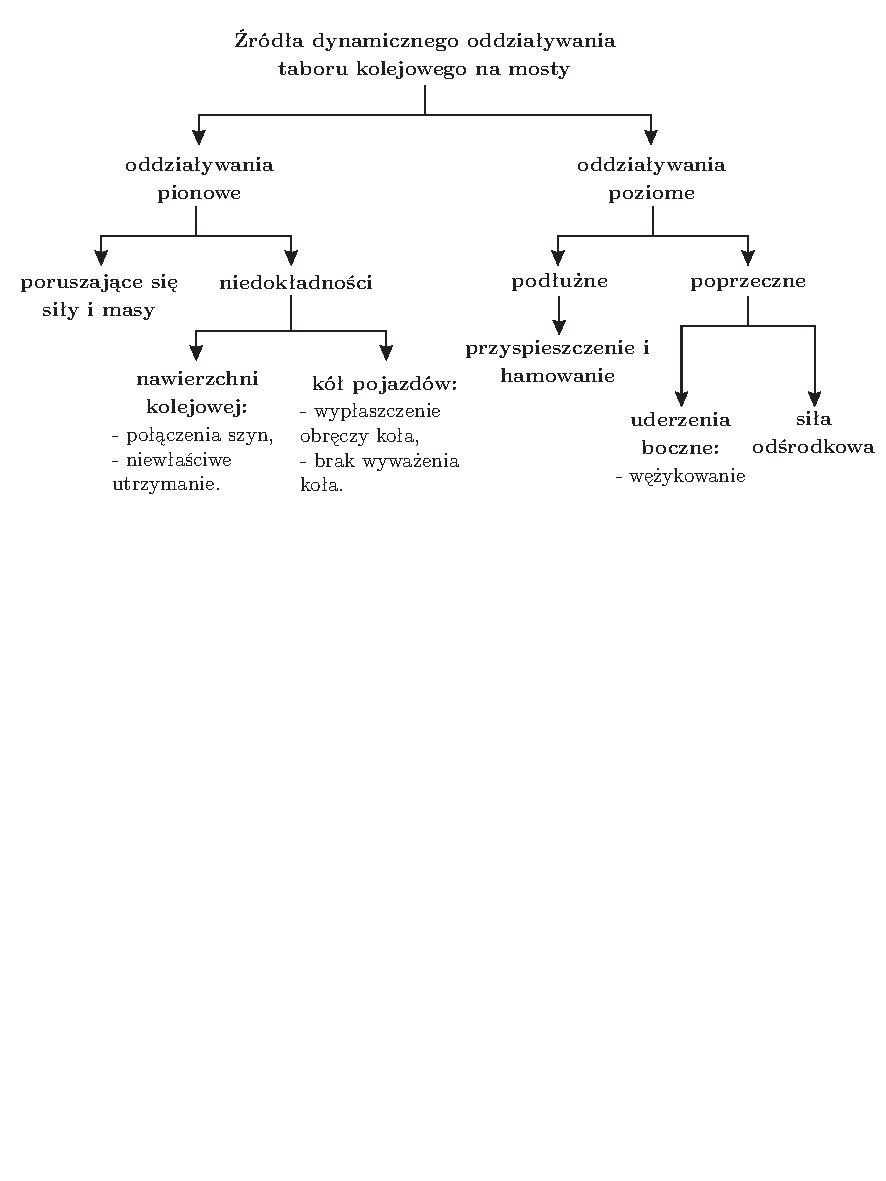
\includegraphics[width=\textwidth]{/dynamic_railway/railway_bridges_forces_croped.pdf} 
	\captionsetup{justification=centering}
	\caption{Zestawienie efektów dynamicznych działających na konstrukcję mostu w trakcie przejazdu taboru kolejowego (na podstawie \parencite{Ladislav1996}) \textbf{UZUPEŁNIĆ}}
	\label{fig:railway_dynamic_forces}
\end{figure}


Pierwsze z nich utożsamiane jest z normowym Stanem Granicznym Nośności, a drugie ze Stanem Granicznym Użytkowania \parencite{PolskiKomitetNormalizacyjny2004}. 


\subsection{Efekty dynamiczne w mostach kolejowych}
Obecnie rozważania dotyczące oddziaływań taboru na mostu kolejowe skupiają się przede wszystkim na obiektach projektowanych wzdłuż Linii Dużych Prędkości (LDP) lub ogólniej dotyczących Kolei Dużych Prędkości (KDP). Oczywiście od wielu lat w przypadku wszystkich mostów kolejowych w trakcie projektowania należy sprawdzić dwa główne kryteria: po pierwsze wytrzymałości i trwałości konstrukcji i po drugie bezpiecznego i komfortowego użytkowania. W ramach pierwszego sprawdzane są zwykle wytrzymałość materiałów, stateczność i deformacje konstrukcji oraz wykonywane są analizy zmęczeniowe \parencite{Ladislav2008}.

Drugie kryterium jest znacznie bardziej złożone i restrykcyjne w przypadku mostów w ciągu LDP. Poza relatywnie prostym w zrozumieniu komfortem pasażera, wymaga ono sprawdzenia bezpieczeństwa nawierzchni kolejowej na moście. Zakłada się, że nawierzchnia jest bezpieczna jeśli jest stabilna i wskutek przejazdu nie nastąpi ryzyko zerwania kontaktu pomiędzy szyną i kołem \parencite{Ramondenc2008}. Przy regularnie utrzymywanym torze, utrata stabilności nawierzchni może nastąpić przede wszystkim w przypadku rozluźnienia podsypki. Pierwszy raz z tym problemem zetknięto się w trakcie utrzymania obiektów mostowych w ciągu trasy francuskiego TGV \parencite{Ramondenc1998}. Zauważono, że tor wymagał znacznie częstszych niż zwykle prac konserwacyjnych. Przeprowadzono badania, w których wykazano, że przy przyspieszeniach większych niż $0.7g-0.8g$ następuje efekt rozluźnienia podsypki i utrata jej stabilności przez zmniejszenie sił tarcia pomiędzy ziarnami kruszywa \parencite{Zacher2008}. Niestateczność podsypki może skutkować zmniejszeniem siły w styku koła i szyny, a w skrajnym wariancie wykolejeniem się pociągu. Kolejnym czynnikiem mogącym wpłynąć na zaburzenie styku koła z szyną są zmiany geometrii toru wywołane przejazdem taboru po obiekcie. W zależności od typu konstrukcji, schematu statycznego, liczby torów zagadnienie to może różnić się stopniem skomplikowania. Niebezpieczne deformacje mogą wynikać z ugięcia wspornika za osią podparcia mostu, z obrotu konstrukcji na łożysku wskutek ugięcia przęsła, ze skręcenia toru po długości obiektu czy ze zmiany krzywizny w planie. Dodatkowo z uwagi na możliwość wystąpienia rezonansu pomiędzy drganiami poprzecznymi mostu i pojazdem szynowym ogranicza się minimalną częstotliwość poprzecznych drgań własnych mostu \parencite{Goicolea2003,Dias2007,Dias2008}. 
\parencite{Niemierko} podaje, że już na etapie projektowania należy rozważyć następujące wartości związane z bezpieczeństwem i komfortem przejazdu pojazdu szynowego:
\begin{itemize}[noitemsep]
	\item przyspieszenia przęsła,
	\item pionowe ugięcia pomostu,
	\item reakcje (uniemożliwić odrywanie na łożyskach),
	\item przemieszczenia wspornika przęsła poza osią podparcia,
	\item kąty skręcenia przęsła,
	\item kąty obrotu na łożyskach,
	\item przemieszczenia wzdłuż osi podłużnej mostu,
	\item ugięcie w poprzek mostu,
	\item kąt obrotu przęsła w poziomie,
	\item częstotliwości drgań własnych konstrukcji.
\end{itemize}

Uwzględnienie efektów dynamicznych przy projektowaniu i w ocenie mostów może odbywać się na wiele sposobów. Aktualnie uwzględnienie efektów oddziaływań dynamicznych może odbyć się na dwa główne sposoby \parencite{Goicolea2008a}:
\begin{enumerate}
	\item przez zwiększenie odpowiednim współczynnikiem dynamicznym
	\footnote{Dyskusję na temat nazewnictwa dotyczącego różnicy pomiędzy przemieszczeniami statycznymi i dynamicznymi, a w tym m.in.: "współczynnik dynamiczny", "współczynnik nadwyżki dynamicznej" i "współczynnik przewyższenia dynamicznego" w kontekście projektowania i próbnych obciążeń przeprowadzono w pracy \parencite{Poprawa2018}} 
	efektów oddziaływań statycznych od obciążeń ruchomych,
	\item przez wyznaczenie i ocenę odpowiedzi dynamicznej układu pod obciążeniem ruchomym.
\end{enumerate}

Od wielu lat normy polskie jak i zagraniczne posługują się współczynnikiem dynamicznym do uwzględnienia efektów dynamicznych przy projektowaniu mostów \parencite{Karas2011}. Metoda polega na zwiększeniu efektów oddziaływania pochodzącego od statycznych modeli obciążeń kolejowych, tak żeby uwzględnić nadwyżkę wynikającą z dynamiki przejazdu po obiekcie. W ten sposób bierze się pod uwagę zarówno wzbudzenie dynamiczne wynikające ze zmienności położenia obciążenia w czasie oraz nierównomierności nawierzchni kolejowej i niedoskonałości kół pojazdów. Należy jednak pamiętać, że podane wzory na wyznaczenie współczynnika dynamicznego zostały wyznaczone dla pojedynczej osi obciążenia ruchomego przejeżdżającego przez obiekt i nie uwzględniają warunków rezonansu \parencite{Goicolea2008}. Jest to uzasadnione rozwiązanie ponieważ zjawisko rezonansu zwykle nie występuje przy przejazdach z prędkością mniejsza nić 200 km/h. Dodatkowo współczynnik dynamiczny nie jest stosowany do obciążeń odwzorowujących rzeczywisty tabor tylko do modeli obciążenia będących obwiednią szerokiej klasy obciążeń kolejowych: pociągów pasażerskich, towarowych i specjalnych. Należy więc pamiętać o jego ograniczeniach stosowalności co ma odzwierciedlenie w obecnych przepisach \parencite{PKNj}. 

Druga rodzina metod opiera na wyznaczeniu odpowiedzi układu pod wpływem przejazdu poprzez wykonanie analizy dynamicznej. Stosowane podejścia różnią się stopniem złożoności i liczbą uwzględnianych czynników \parencite{Goicolea2008a}. Obliczenia mogą odbywać się analitycznie lub za pomocą metod numerycznych. Pojazd może być opisany jako pojedyncza siła pozbawiona inercji, jako masa poruszająca się bezpośrednio po układzie lub też jako oscylator lepko sprężysty odwzorowujący zawieszenie pociągu. Ostatni wariant może być rozbudowywany do większej liczby stopni swobody i o inne elementy interakcji pomiędzy pojazdem, a konstrukcją \parencite{Calcada2008,Szafranski2013,Szafranski2021}. Uwzględnienie resorowania pojazdu szynowego z reguły obniża efekt wzbudzenia obiektu w trakcie przejazdu. Warto jednak zauważyć, że rozważenie interakcji pomiędzy taborem, a konstrukcją nie wpływa zauważalnie na wyniki drgań poza warunkami rezonansu i dla dużych rozpiętości lub konstrukcji ciągłych \parencite{Goicolea2008a}.

Pierwsze rozwiązania analityczne drgań konstrukcji z obciążeniem ruchomym dla elementarnych modeli mechanicznych pojawiły się już XIX w. Prace \parencite{Willis1849,Stokes1849,Saller1921,Timoshenko1922,Inglis1934,Kolousek1973} stanowią kamienie milowe w historii rozwoju metod wyznaczania odpowiedzi w mostach pod obciążeniem ruchomym. Tematyka rozwiązań analitycznych nie będzie rozwijana w niniejszej pracy z uwagi na obszerność zagadnień i dostępną literaturę krajową \parencite{Szczesniak2018}. Metody analityczne ograniczone są do raczej prostych modeli elementarnych i typowych obciążeń. Pomimo, że ich istota w rozwoju badania odpowiedzi dynamicznej mostów oraz ich walory edukacyjne są niekwestionowane, w pracy posiłkowano się bardziej uniwersalnymi metodami numerycznymi. Warto jednak wspomnieć o jednej z najprostszych, a jednocześnie stosunkowo uniwersalnej metodzie wyznaczenia maksymalnych przyspieszeń za pomocą Dynamicznej Sygnatury Pociągu \teng{Dynamic Train Signature} \parencite{Goicolea2008a,ERRI1998}. Chociaż ma ona zastosowanie jedynie do układu belki wolno podpartej to jej niewątpliwą zaletą jest to, że nie wymaga stosowania złożonych metod numerycznych ani zaawansowanego aparatu matematycznego do uzyskania miarodajnych wyników. W metodzie uwzględnia się charakterystyki dynamiczne układu, dynamiczną linię wpływu mostu \teng{dynamic influence line} oraz sygnaturę dynamiczną pociągu. Wspomniana sygnatura dynamiczna pociągu jest funkcją określoną indywidualnie dla danego pociągu i jest niezależna od cech mechanicznych przęsła. Funkcja zależna jest od typowego rozstawu osi pociągu oraz liczby tłumienia układu. Dzięki wyprowadzonym formułom metoda jest przystępna również dla inżynierów niezajmujących się pracą naukową.
W przypadkach złożonych, gdzie metody analityczne nie mają zastosowania aktualnie najbardziej uniwersalną metodą przewidywania odpowiedzi dynamicznej jest wykorzystanie Metody Elementów Skończonych (MES). MES umożliwia dyskretyzację konstrukcji dzieląc ją na węzły i elementy skończone. Dzięki temu możliwe jest sformułowanie różniczkowego równania ruchu dla układu o wielu stopniach swobody (MDOF) danego wzorem (\ref{eq: mot_und_num}). Podstawowe metody rozwiązania równania ruchu MDOF opierają się na bezpośrednim całkowaniu numerycznym (metoda Newmarka) lub superpozycji modalnej. Obie metody opisano w punkcie \ref{section: mdof_response}. Metoda Elementów Skończonych pozwala na opis skomplikowanych struktur, zadanie różnorodnych obciążeń i wybór odpowiedniego rodzaju analizy. Możliwe jest rozwiązywanie zarówno układów liniowych jak i nieliniowych. Z uwagi na swoją skuteczność została zaimplementowana w wielu komercyjnych programach do analizy konstrukcji. Istnieje obszerny zbiór zagranicznych pozycji bibliograficznych opisujących fundamentalne sformułowania MES \parencite{Zienkiewicz2005,Hughes1987,Langtangen2019,Hartmann2007}, a także w języku polskim \parencite{Kleiber1985,Rakowski2016}. 


\subsection{Przepisy normowe i wytyczne}
Po omówieniu przyczyn, efektów i metod przewidywania drgań konstrukcji należy odnieść się do aktualnego stanu prawnego. Obecnie w Polsce obowiązuje szereg norm i zarządzeń opisujących elementy projektowania, dostosowywania i utrzymania obiektów kolejowych w ciągu Linii Dużych Prędkości \parencite{PolskieLinieKolejoweS.A.2005,PolskieLinieKolejoweS.A.2009,PolskiKomitetNormalizacyjny,PolskiKomitetNormalizacyjny2004,PKNj}. Szczegółową analizę zapisów dotyczących uwzględniania zachowania dynamicznego mostów kolejowych według polskich przepisów opisali w swoich pracach \cite{Oleszek2015,Oleszek2015b,Oleszek2016a}. Aktualnie obowiązujące Eurokody w części poświęconej dynamice mostów kolejowych opierają się na badaniach i doświadczeniach członków Europejskiego Instytutu Badawczego Kolejnictwa \teng{European Railway Research Institute (ERRI)} \parencite{ERRI1998,Muncke2008}, Międzynarodowego Związku Kolei \teng{International Union of Railwais, fr. Union Internationale des Chemins de fer (UIC)} \parencite{UnionInternationaleDesCheminsDeFer2006,UnionInternationaleDesCheminsDeFer2009}. Szczegółową historię ewolucji przepisów do postaci aktualnie występującej w normach europejskich oraz ich interpretację przedstawił w pracy doktorskiej \cite{James2003}. Również bardzo obszerny opis zagadnienia można znaleźć w \parencite{Goicolea2002,Dias2007}.

\cite{Karas2011a} określił podejście dotyczące uwzględniania efektów dynamicznych przedstawione w Eurokodach jako kompromis. Z jednej strony w niektórych przypadkach stosuje się tradycyjną metodę zwiększenia efektu oddziaływań statycznych za pomocą współczynnika dynamicznego, z drugiej zaś strony niekiedy wymagane jest stosowanie nowoczesnych metod wyznaczania bezpośrednio odpowiedzi konstrukcji pod obciążeniem dynamicznym. Ostatecznie jednak norma nakazuję porównanie efektów obliczeń obiema metodami i uznaje za decydujący przypadek bardziej niekorzystny. 

\subsubsection{Algorytm wyboru zakresu analiz}
W normie PN-EN 1991-2 wyraźnie określono w punkcie 6.4.5.1(1), że współczynnik dynamiczny nie uwzględnia efektów rezonansu. Jednocześnie zdając sobie sprawę z czasochłonności pełnej analizy dynamicznej spróbowano ograniczyć jej wykonanie do przypadków nietypowych i zagrożonych nadmiernymi drganiami. Wprowadzono algorytm decydujący o wyborze metody uwzględnienia efektów dynamicznych. Zastosowano szereg kryteriów, po których spełnieniu można pominąć wyznaczenie odpowiedzi dynamicznej konstrukcji, a efekty przejazdu uwzględnia się za pomocą współczynnika dynamicznego. Algorytm opisujący ścieżkę postępowania zawartą w normie przytoczono na rysunku \ref{fig:ec_algorithm_dyna}, gdzie: $V$ - miejscowa maksymalna prędkość liniowa [km/h], $L$ - rozpiętość przęsła [m], $n_0$ - pierwsza częstotliwość giętnych drgań własnych mostu [Hz], $n_T$ - pierwsza częstotliwość skrętnych drgań własnych mostu [Hz], $v$ - maksymalna prędkość nominalna [m/s], $(v/n_0)_lim$ - wg załącznika F normy. Samodzielne liczby w nawiasach okrągłych (1) - (7) oznaczają uwagi przytoczone w normie w sąsiedztwie diagramu. Zgodnie z przedstawionym schematem kluczowymi parametrami potrzebnymi do podjęcia decyzji o wykonaniu analizy dynamicznej są:
\begin{itemize}[noitemsep]
	\item maksymalna miejscowa prędkość na linii,
	\item schemat statyczny konstrukcji,
	\item rozpiętość przęsła,
	\item pierwsza częstotliwość giętnych drgań własnych $n_0$,
	\item pierwsza częstotliwość skrętnych drgań własnych $n_T$
\end{itemize}
\begin{figure}[p]
	\centering
	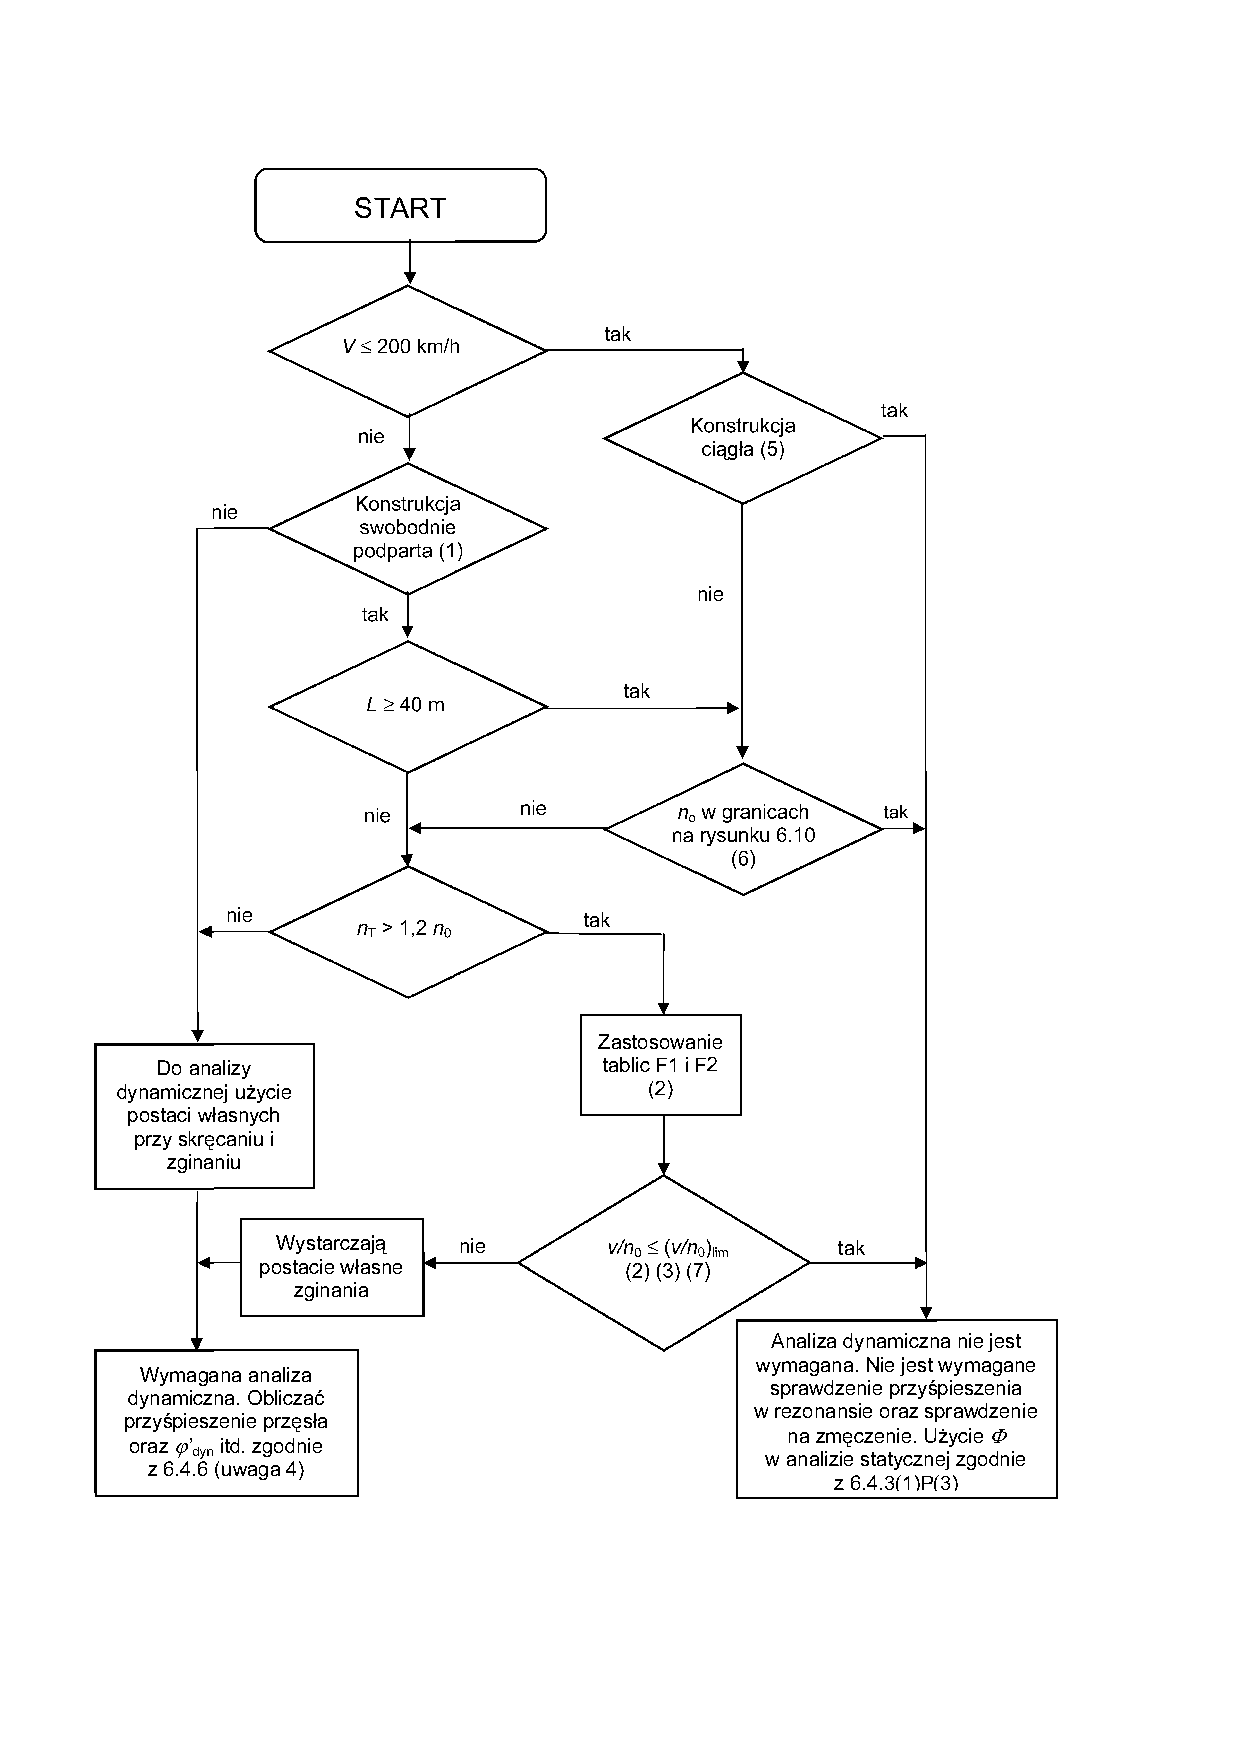
\includegraphics[width=\textwidth]{/dynamic_railway/ec_algorithm_dyna.pdf} 
	\captionsetup{justification=centering}
	\caption{Algorytm określający czy wymagana jest analiza dynamiczna wg \parencite{PKNj}}
	\label{fig:ec_algorithm_dyna}
\end{figure}

Po ustaleniu wszystkich parametrów schemat decyzyjny wskazuje ewentualną konieczność wykonania analizy dynamicznej. Algorytm zależnie od ich wartości realizuje wiele scenariuszy. Można jednak wyodrębnić poszczególne sytuacje, które wynikają z algorytmu i mają potwierdzenie we wcześniej przytoczonych badaniach i opracowaniach. Poniżej krótko omówiono kluczowe aspekty mechanizmu decyzyjnego. 

Schemat statyczny wpływa na przebieg procesu wyboru w dwóch miejscach. Po pierwsze konstrukcja może być ciągła lub swobodnie podparta. Po drugie, swobodnie podparte przęsło może różnić się stopniem skomplikowania układu. Roboczo w tej pracy rozróżniono je i nazwano jako konstrukcje \enquote{proste} bądź \enquote{złożone}. Konstrukcja określona jako \enquote{prosta} to zgodnie z normą taka, której schematem statycznym jest \textit{belka swobodnie podparta zachowująca się tylko jak prosta belka podłużna lub prosta płyta z pomijalnymi efektami skosu na podporach niepodatnych}. W przeciwnym wypadku konstrukcja jest \enquote{złożona}.

Do wyznaczenia częstotliwości i postaci drgań własnych niezbędne jest wykonanie analizy modalnej (p. \ref{sect:modal_analysis}). Dla złożonych układów wykonywana jest ona zazwyczaj w programach MES. Dodatkowo, w niektórych sytuacjach proces decyzyjny pozwala pominąć analizę dynamiczną opierając się na nomogramie (rys. \ref{fig:ec_algorithm_dyna_boundary}) oraz Załączniku F do normy PN-EN 1991-2. Nomogram pokazuje obszar stosowalności współczynników dynamicznych w zależności od częstotliwości pierwszej giętnej postaci drgań własnych w funkcji rozpiętości przęsła. Innymi słowy jeżeli pierwsza częstotliwość giętnych drgań własnych obiektu o konstrukcji 'prostej' i danej rozpiętości mieści się pomiędzy dolną, a górną granicą zakreskowanego obszaru, to współczynniki dynamiczne $\phi '$ i $\phi ''$ zdefiniowane przez normę są miarodajne i analiza dynamiczna nie jest wymagana. Granica górna nomogramu jest związana z nierównościami toru, a granica dolna ujmuje dodatkowe oddziaływanie wynikające z samej dynamiki przejazdu. W przypadku prędkości większych niż 200 km/h nomogram ma zastosowanie do obiektów krótkich ($L<=40$ m). Przy odpowiednim stosunku częstotliwości drgań skrętnych i giętnych ($n_T>1.2n_0$) możliwe jest pominięcie analizy dynamicznej z wykorzystaniem załącznika F do normy. W załączniku F zestawiono współczynniki graniczne $(v/n_0)_lim$, gdzie $v$ - maksymalna prędkość nominalna taboru. Współczynniki graniczne zostały zdefiniowane i zestawione w tablicach F.1 i F.2 normy. Wyznaczono je dla 'prostych' obiektów o zróżnicowanych - lecz nieograniczonych - rozpiętościach oraz dla różnych ułamków tłumienia i różnych zastępczych obciążeń równomiernie rozłożonych przypadających na metr bieżący mostu. Według algorytmu jeżeli dla obliczanego obiektu spełnione jest $(v/n_0)>(v/n_0)_lim$ to analiza dynamiczna nie jest wymagania, ponieważ efekt obciążenia będzie mniejszy niż przy obciążeniu statycznym LM 71 z odpowiednim współczynnikiem dynamicznym. Wartości graniczne zostały wyznaczone przy uwzględnieniu współczynników bezpieczeństwa dla kryteriów przyspieszenia, ugięcia i wytrzymałości, dla starannie utrzymanego toru i częstotliwości $n_0$ mniejszej niż górna granica nomogramu (rys. \ref{fig:ec_algorithm_dyna_boundary}. Do analiz użyto 7 pociągów rzeczywistych A-F również przedstawionych w załączniku F. 
\begin{figure}[h]
	\centering
	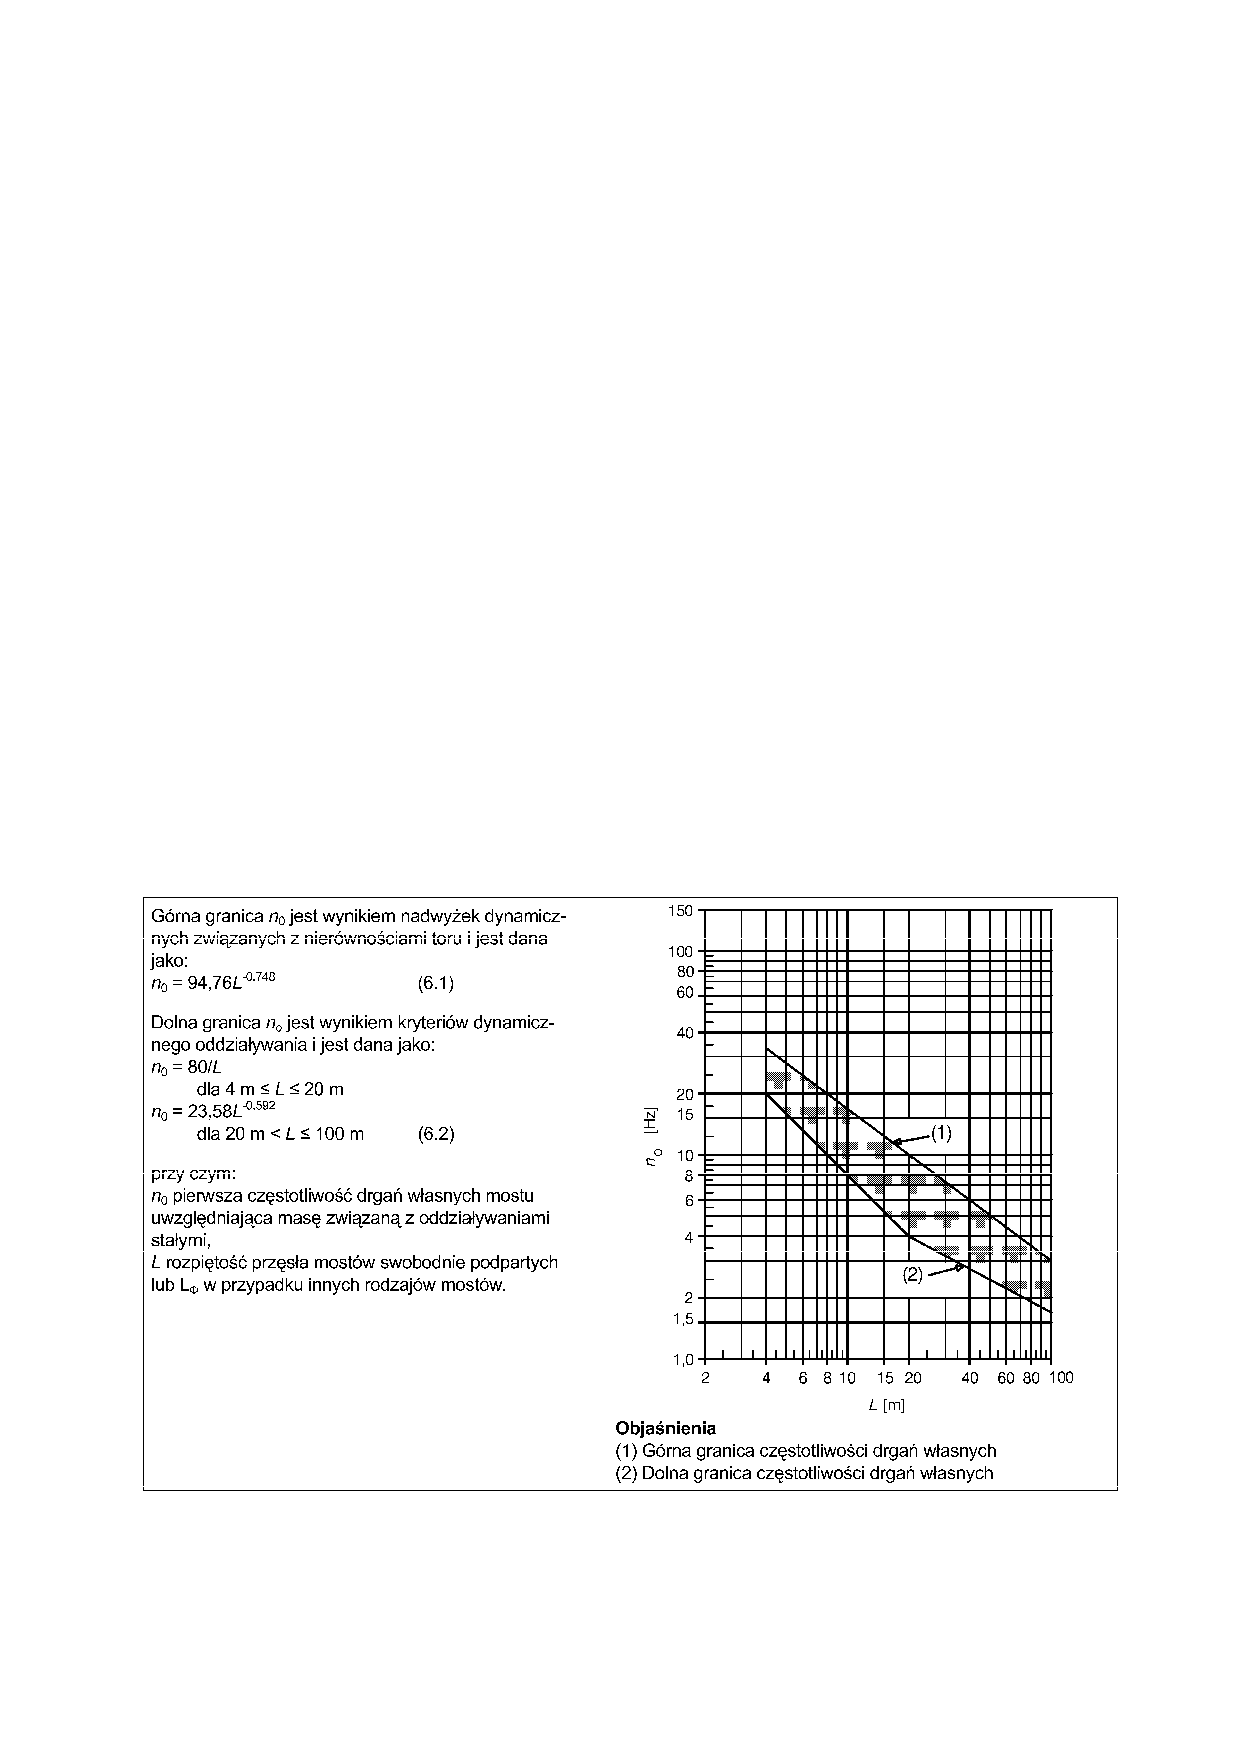
\includegraphics[width=\linewidth]{/dynamic_railway/ec_algorithm_dyna_boundary.pdf} 
	\captionsetup{justification=centering}
	\caption{Granice pierwszej częstotliwości drgań własnych mostu określone w normie \cite{PKNj}}
	\label{fig:ec_algorithm_dyna_boundary}
\end{figure}

Nomogram (rys. \ref{fig:ec_algorithm_dyna_boundary}) oraz tablice w załączniku F, powstały na bazie wielu lat badań i doświadczeń naukowców i inżynierów zajmujących się tematyką drgań mostów kolejowych \parencite{UnionInternationaleDesCheminsDeFer2009,ERRI1998}. Dzięki nim zidentyfikowano przypadki konstrukcji dla których nie ma obowiązku ponownego prowadzenia pełnej analizy dynamicznej. Mimo że dotyczy to jedynie prostych, powtarzalnych konstrukcji, to w typowych przypadkach pozwala zaoszczędzić projektantom mnóstwo czasu. Z drugiej strony, przy maksymalnej prędkości większej od 200 km/h analiza dynamiczna musi być wykonana jeśli:
\begin{itemize}[noitemsep]
	\item konstrukcja jest \enquote{złożona},
	\item konstrukcja jest \enquote{prosta}, rozpiętość jest mała ($L < 40$ m), a częstotliwość drgań skrętnych jest bliska częstotliwości drgań giętnych ($n_T<1.2n_0$),
	\item konstrukcja jest \enquote{prosta}, rozpiętość jest duża ($L < 40$ m), ale częstotliwość giętnych drgań własnych nie mieści się w wyznaczonych granicach (Rys. \ref{fig:ec_algorithm_dyna_boundary}) i częstotliwość drgań skrętnych jest bliska częstotliwości drgań giętnych ($n_T<1.2n_0$).
\end{itemize}




\subsubsection{Obciążenia} \label{sect: eurokod_obciazenia_dyn}
W pracy poruszany jest temat optymalizacji struktury obiektów mostowych, który zdecydowanie częściej może być rozważany na etapie projektowania mostu niż w trakcie jego życia. Z tego względu w dalszej części pracy rozważone zostaną obciążenia służące projektowaniu, a nie sprawdzaniu istniejących konstrukcji. Według rozporządzenia \parencite{PolskiKomitetNormalizacyjny} do projektowania należy używać modeli obciążeń zawartych w omawianej już normie PN-EN 1991-2, a do sprawdzania nośności istniejących obiektów kolejowych modeli obciążeń eksploatacyjnych opisanych w normie PN-EN 15528 \parencite{PolskiKomitetNormalizacyjnya,uszczki2015}. Norma \cite{PolskiKomitetNormalizacyjnya} zawiera instrukcje i przepisy pozwalające zaklasyfikować pojazdy i linie kolejowe do odpiewdnich klas.

W normie PN-EN 1991-2 występuję kilka obciążeń kolejowych podzielonych na dwie grupy w zależności od przeznaczenia. Pierwszą grupę stanowią obciążenia do analiz statycznych. W jej skład wchodzą modele obciążenia: UIC 71, SW/0, SW/2 i pociąg bez ładunku. Model UIC 71 został opracowany już w 1971 roku \parencite{UnionInternationaleDesCheminsDeFer2006} i był stosowany w poprzedniej generacji Polskich Norm \parencite{PKNe}. Z tego względu jest dobrze znany środowisku projektowemu i zwykle nie występują problemy w jego zastosowaniu. Obciążenia statyczne nie stanowią głównego tematu niniejszej pracy i nie będą szerzej omawiane. Ich szczegółowy opis, pochodzenie oraz zasady użycia można znaleźć w normie PN-EN 1991-2 oraz pracach \parencite{James2003,UnionInternationaleDesCheminsDeFer2006}. Druga grupa zawiera modele obciążeń wykorzystywane w analizach dynamicznych lub zmęczeniowych. Zaliczają się do niej:
\begin{itemize}[noitemsep]
	\item Pociągi Uniwersalne HSLM-A i HSLM-B (PN-EN 1991-2 p. 6.4.6.1.1),
	\item Pociągi Rzeczywiste (PN-EN 1991-2 załącznik F)
	\item Pociągi Zmęczeniowe\footnote{Odniesienie do Pociągów Zmęczeniowych w kontekście analizy dynamicznej znajduje się w punkcie 6.4.6.1.1(7) normy. Mówi on o zalecanych obciążeniach w przypadku kiedy analiza dynamiczna jest wymagana, a maksymalna prędkość jest mniejsza niż 200 km/h. W angielskiej wersji tekstu pojawia się zdanie "Train Types 1 to 12 given in annex D", które wyraźnie odnosi się do Pociągów Zmęczeniowych. W polskiej wersji zdanie to zostało przetłumaczone jako "Pociągi Typowe od 1 do 12 podane w załączniku D". Pojęcie Pociąg Typowy występuje również w załączniku D w odniesieniu do jednego z rodzajów Pociągów Rzeczywistych. Racjonalne wydaje się dosłowne stosowanie przepisu w jego angielskiej formie.} (PN-EN 1991-2 załącznik D). 
\end{itemize}

Opis obciążeń dynamicznych należy rozpocząć od przywołania idei interoperacyjności. Zgodnie z dyrektywą Rady Unii Europejskiej 96/48/WE z 1996 roku opracowane opracowano Warunki Techniczne Interoperacyjności \teng{Technical Specifications of the Interoperability (TSI)} \parencite{Muncke2008}. Mają one założeniu ujednolicić dotychczas zróżnicowane systemy kolejowe państw członkowskich Unii Europejskiej. Dzięki wdrożeniu idei ułatwione miałoby być podróżowanie pomiędzy krajami Unii bez utrudnień związanych z zastosowaniem różnych rozwiązań technicznych. Zgodnie z Warunkami TSI wszystkie obiekty kolejowe powinny być zwymiarowane na obciążenie statyczne LM71 oraz pozwolić na liniach dużych prędkości na ruch wszystkich aktualnie występujących i mogących wystąpić w przyszłości pociągów dużych prędkości.

Pierwszą grupą obciążeń normowych używanych do analiz dynamicznych są Pociągi Rzeczywiste. Pociągi dużych prędkości występujące na europejskich liniach mogą być podzielone na trzy grupy taboru w zależności od wzajemnego usytuowania wózków i wagonów \parencite{Goicolea2008a}. Schematy pociągów zawarto w normie PN-EN 1991-2 załącznik E i przytoczono na rysunku \ref{fig:train_types_EC}. Poszczególne grupy można opisać następująco (w nawiasach podano przykłady rzeczywistego taboru):
\begin{itemize} [noitemsep]
	\item pociągi przegubowe - dwa wagony połączone są jednym wózkiem znajdującym się między nimi (THALYS, AVE i EUROSTAR),
	\item pociągi typowe - każdy wagon posiada dwa własne wózki (ICE2, ETR500),
	\item pociągi regularne - brak wózków, wagony są oparte na pojedynczych osiach znajdujących się na połączeniu wagonów (TALGO).
\end{itemize}
\begin{figure}[h]
	\centering
	\subfloat[]{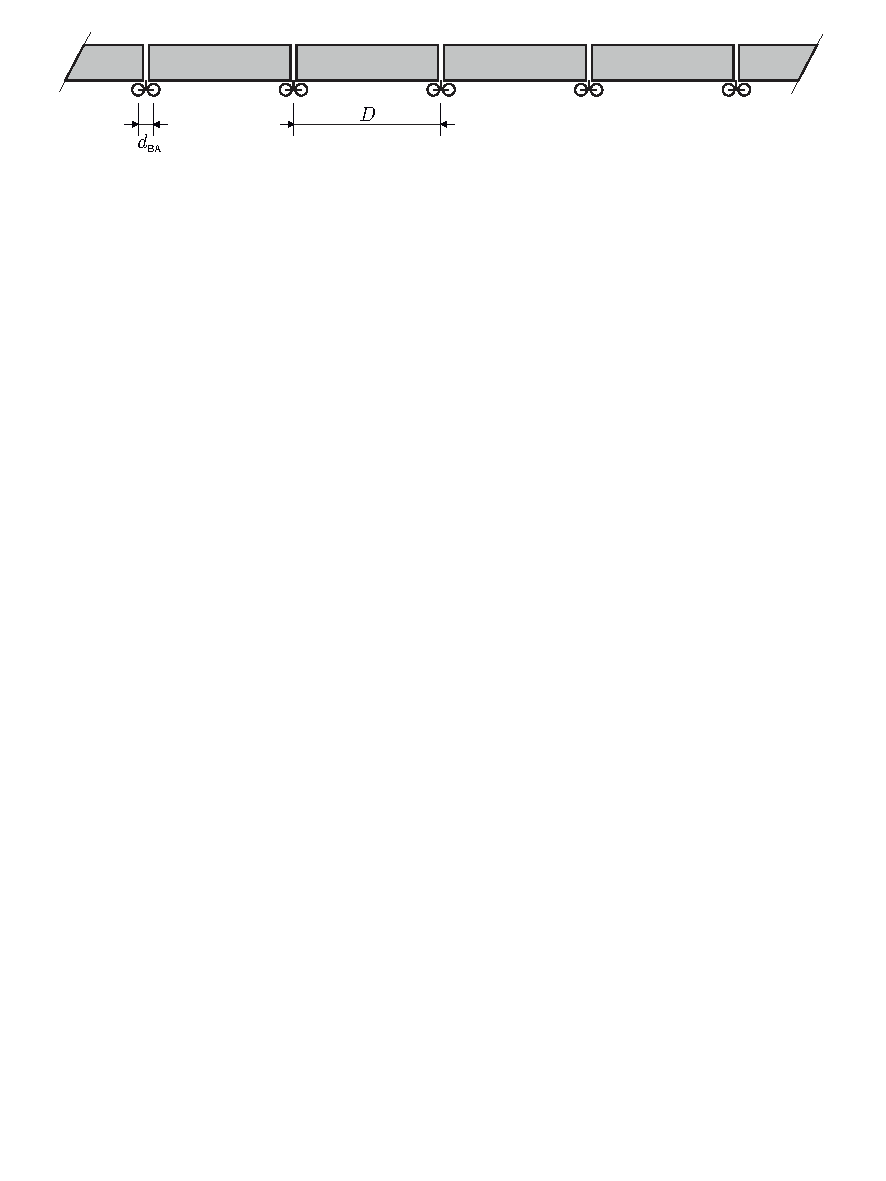
\includegraphics[]{/dynamic_railway/types_of_trains_articulated.pdf}  \label{fig:train_types_EC_art} } \\
	\subfloat[]{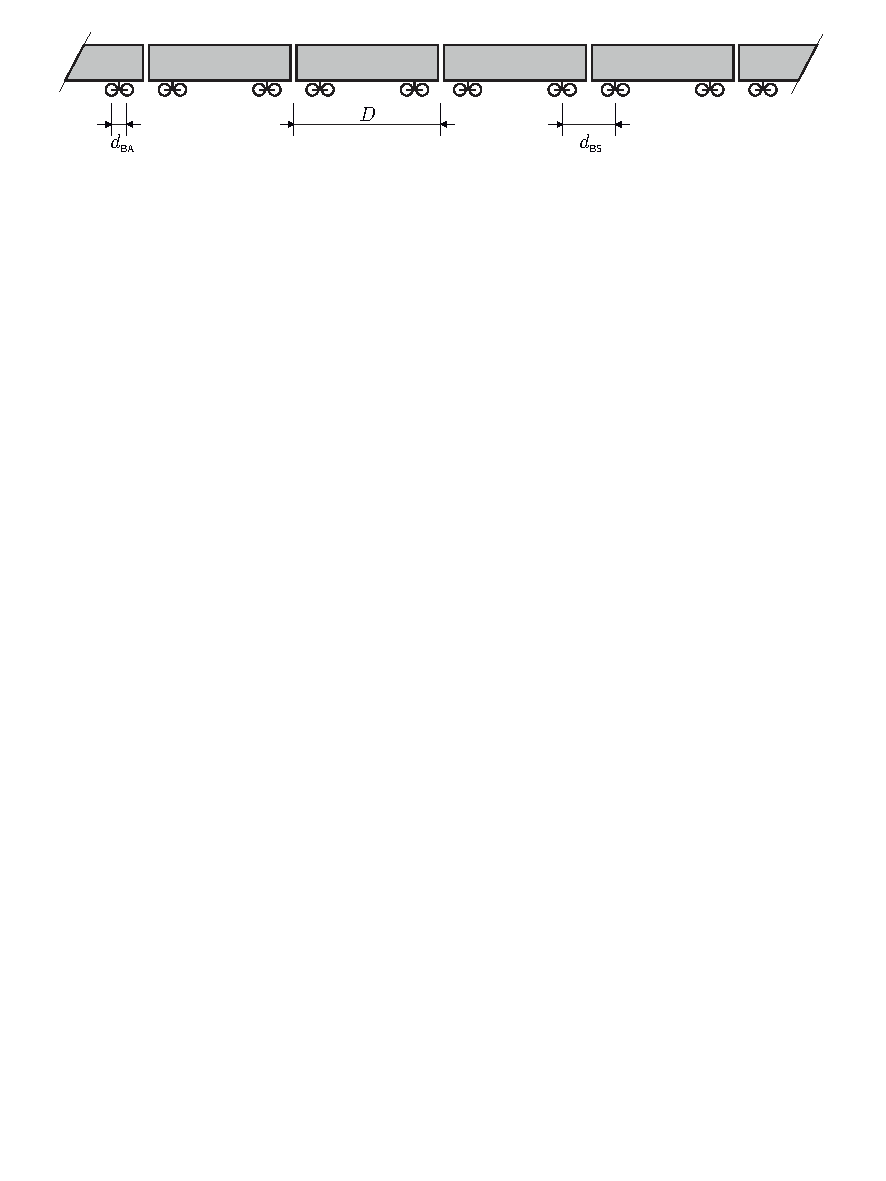
\includegraphics[]{/dynamic_railway/types_of_trains_conventional.pdf}} \\
	\subfloat[]{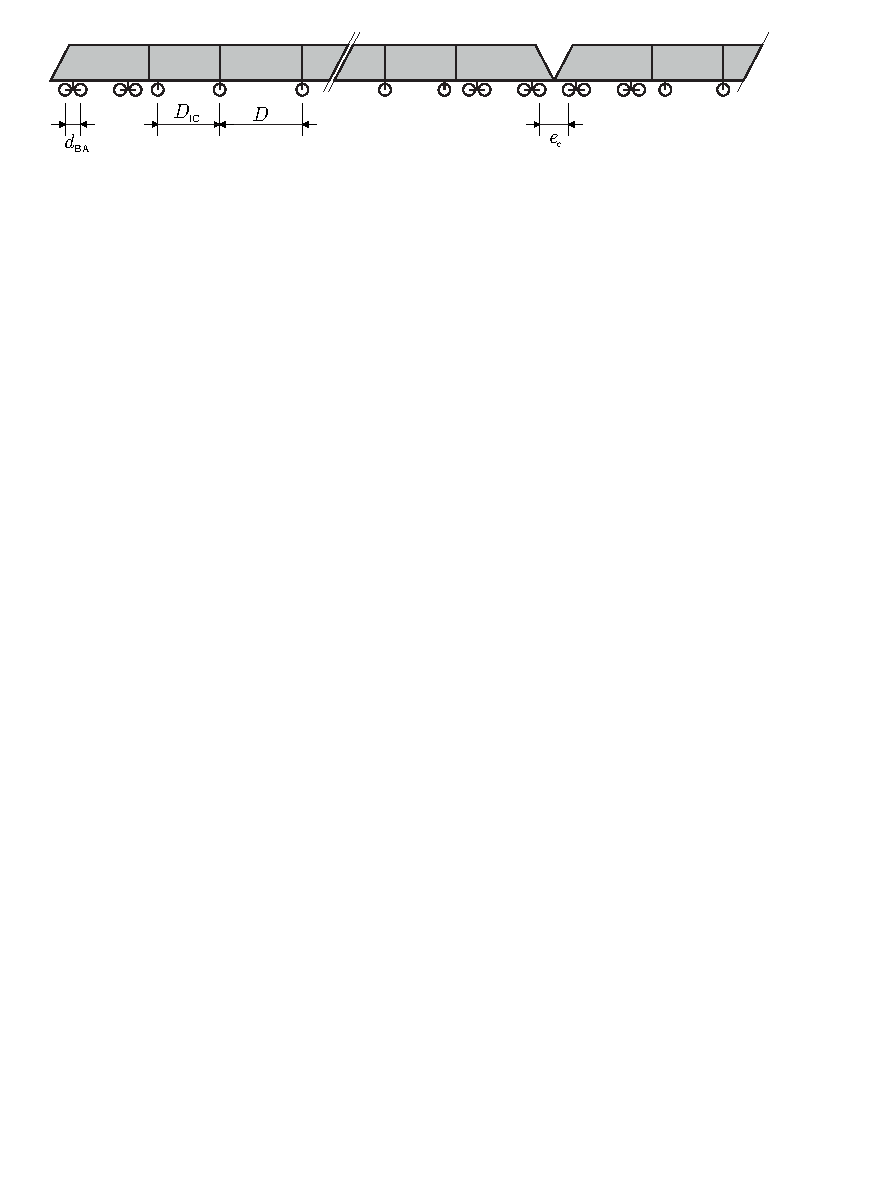
\includegraphics[]{/dynamic_railway/types_of_trains_regular.pdf}}
	\captionsetup{justification=centering}
	\caption{Typy pociągów rzeczywistych kursujących na Europejskich liniach dużych prędkości: (a) pociąg przegubowy; (b) pociąg typowy; (c) pociąg regularny. Oznaczenia: $d_{BA}$ - rozstaw osi w wózku, $D$ - odległość miedzy regularnie odległymi osiami lub długość wagonu, $D_{IC}$ - długość wagonu pośredniego, $e_c$ - odległość między sąsiednimi osiami dwóch pojedynczych zestawów pociągów \parencite{PKNj}.}
	\label{fig:train_types_EC}
\end{figure}
Na liniach kolejowych o prędkości maksymalnej mniejszej niż 200 km/h zarządca w indywidualnej dokumentacji technicznej może określić Pociągi Rzeczywiste, które należy uwzględnić w analizach.

\begin{figure}[h]
	\centering
	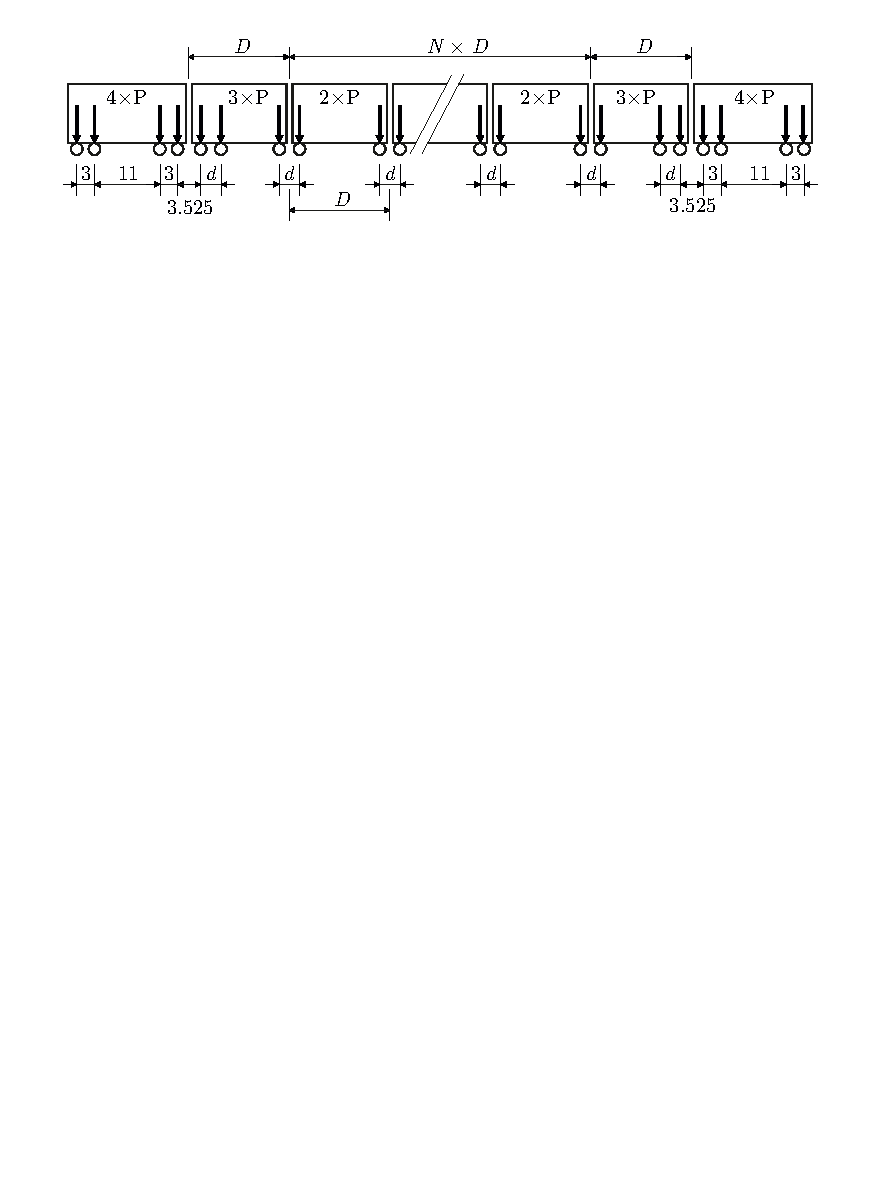
\includegraphics[]{/dynamic_railway/hslm_a.pdf}
	\captionsetup{justification=centering}
	\caption{Model pociagu HSLM-A według PN-EN 1991-2. Na podstawie \cite{PKNj}}
	\label{fig:train_hslm_a}
\end{figure}

\begin{figure}[h]
	\centering
	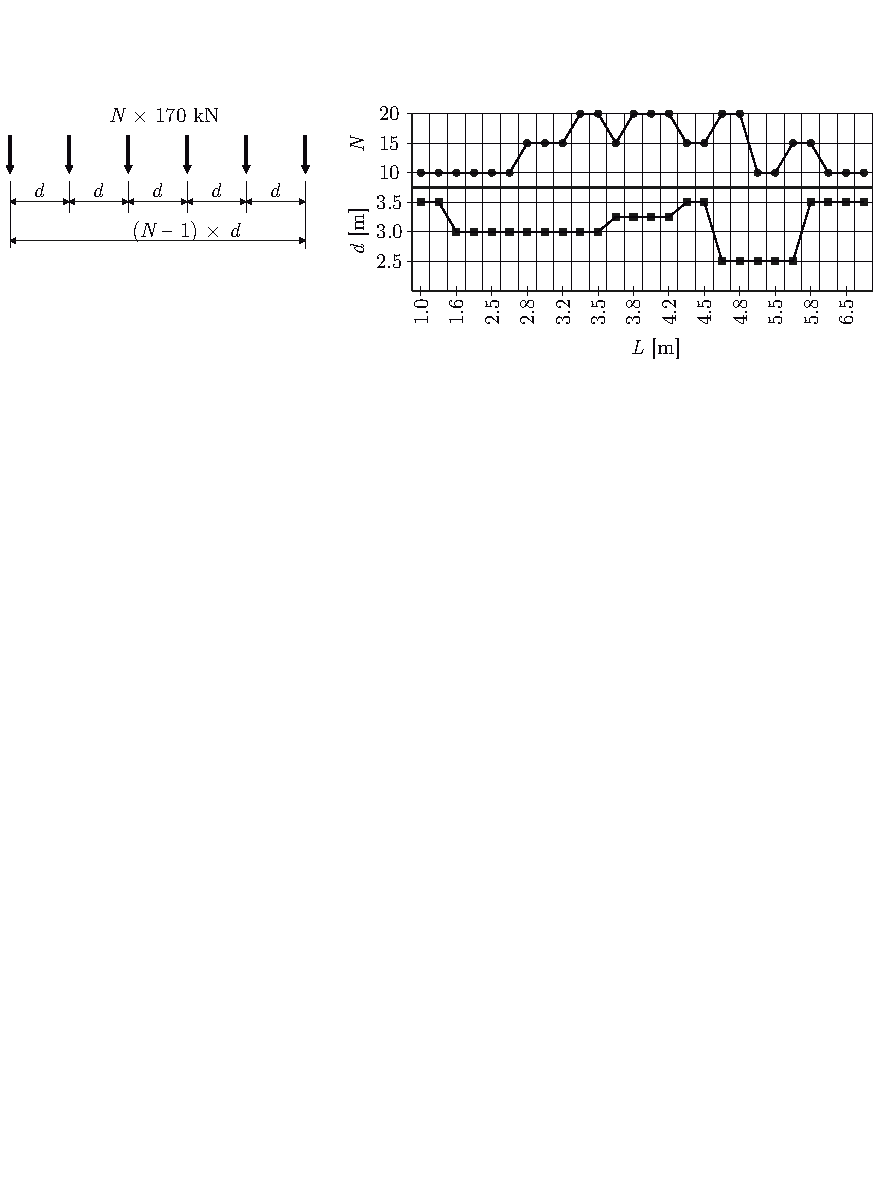
\includegraphics[]{/dynamic_railway/hslm_b.pdf}
	\captionsetup{justification=centering}
	\caption{Model pociagu HSLM-B według PN-EN 1991-2. Na podstawie \cite{PKNj}}
	\label{fig:train_hslm_b}
\end{figure}

\begin{table}[]
	\caption{Parametry modelu HSLM-A wg \cite{PKNj}}
	\centering
	\footnotesize
	\begin{tabular}{@{}ccccc@{}}
		\toprule
		HSLM & \begin{tabular}[c]{@{}c@{}}Liczba pośrednich\\ wagonów pasażerskich \\ $N$\end{tabular} & \begin{tabular}[c]{@{}c@{}}Długość wagonu\\ pasażerskiego \\ $D$ {[}m{]}\end{tabular} & \begin{tabular}[c]{@{}c@{}}Rozstaw osi\\ wózków \\ $d$ {[}m{]}\end{tabular} & \begin{tabular}[c]{@{}c@{}}Siła skupiona \\ $P$ {[}kN{]}\end{tabular} \\ \midrule
		A1   & 18                                                                                      & 18                                                                                    & 2,0                                                                         & 170                                                                   \\ \midrule
		A2   & 17                                                                                      & 19                                                                                    & 3,5                                                                         & 200                                                                   \\ \midrule
		A3   & 16                                                                                      & 20                                                                                    & 2,0                                                                         & 180                                                                   \\ \midrule
		A4   & 15                                                                                      & 21                                                                                    & 3,0                                                                         & 190                                                                   \\ \midrule
		A5   & 14                                                                                      & 22                                                                                    & 2,0                                                                         & 170                                                                   \\ \midrule
		A6   & 13                                                                                      & 23                                                                                    & 2,0                                                                         & 180                                                                   \\ \midrule
		A7   & 13                                                                                      & 24                                                                                    & 2,0                                                                         & 190                                                                   \\ \midrule
		A8   & 12                                                                                      & 25                                                                                    & 2,5                                                                         & 190                                                                   \\ \midrule
		A9   & 11                                                                                      & 26                                                                                    & 2,0                                                                         & 210                                                                   \\ \midrule
		A10  & 11                                                                                      & 27                                                                                    & 2,0                                                                         & 210                                                                   \\ \bottomrule
	\end{tabular}
	\label{tab:hslm_a_parameters}
\end{table}

Drugą grupę obciążeń stosowanych w analizach dynamicznych stanowią pociągi uniwersalne \teng{Universal Trains}. W jej skład wchodzą dwa modele HSLM-A i HSLM-B \teng{High Speed Load Model (HSLM)}. Są to teoretyczne modele, które powstały aby zagwarantować spełnienie warunków interoperacyjności kolei w państwach Unii Europejskiej. Odzwierciedlają szeroki zakres obciążeń od pociągów dużej prędkości aktualnie użytkowanych i potencjalnie występujących w przyszłości. Model HSLM-A został przedstawiony na rysunku \ref{fig:train_hslm_a} i występuje w 10 wariantach różniących się parametrami - oznaczonych od A1 do A10. Parametry dla modelu HSLM-A przedstawono w tabeli \ref{tab:hslm_a_parameters}. Model obciążenia stanowi potok sił, w wiekszości rozstawionych w regularny sposób jak dla osi kół pociagu. Schemat rozkładu sił odpowiada pociągowi o typie przegubowym (rys. \ref{fig:train_types_EC_art}). Całkowita długość pociągu w każdym z wariantów wynosi około 400 m i zależy od liczby wagonów $N$ i ich długości $D$. Obciążenie przypadające na oś oznaczono jako $P$, a jego wartość miesci się w zakresie od 170 kN do 210 kN. Rozstaw osi wózków $d$ również został zróżnicowany od 2 do 3.5 m. Dodatkowo na początku i na końcu modelu znajduje się nieregularny układ sił odwzorowujący lokomotywy. Model HSLM-B pokazano na rysunku \ref{fig:train_hslm_b}. Składa się z $N$ sił w regularnym rozstawie $d$. Parametry modelu $d$ i $N$ przyjmuje się w zależności od rozpiętości przęsła $L$ zgodnie z rysunkiem \ref{fig:train_hslm_b}. Model HSLM-B zgodnie z zaleceniem stosowany może być dla obiektów 'prostych' o rozpiętości poniżej 7 m. Dla pozostałych obiektów zalecane jest wyznaczenie odpowiedzi od obciążenia modelem HSLM-A dla wszystkich wariantów A1-A10.

\subsubsection{Parametry analizy dynamicznej}

Do analiz dynamicznych należy zastosować obciążenia Pociągami Rzeczywistymi występującymi na linii oraz modele HSLM jeśli dla linii stosowane są międzyoperacyjne kryteria europejskie dużych prędkości. Jeśli analiza dynamiczna jest wymagana, a prędkość liniowa jest mniejsza nż 200 km/h to do sprawdzenia efektów dynamicznych należy zastosować Pociągi Rzeczywiste A-F (załącznik F normy \cite{PKNj}) oraz Pociągi Zmęczeniowe 1-12 (załącznik D normy \cite{PKNj}).


Prędkości analizowanego przejazdu należy przyjmować od 40 km/h do maksymalnej prędkości obliczeniowej co 10 km/h. Maksymalną prędkość obliczeniową zaleca się przyjmować jako $1.2\times\,$\textit{maksymalna dopuszczalna prędkość pojazdu}. W pobliżu prędkości rezonansowych (\ref{eq:criticla_speed}) należy zagęścić obliczenia. Według przepisów \parencite{PKNj,UnionInternationaleDesCheminsDeFer2009} przyspieszenia powinny być wyznaczone w zakresie częstotliwości sygnału do $f_{max}=\text{max}\{1.5n_0;n_3; 30\,\text{Hz}\}$, gdzie $n_0$ i $n_3$ oznaczają odpowiednio pierwszą i trzecią postać giętnych drgań elementu. W przypadku mostów zwykle decydujący jest warunek 30 Hz, ponieważ drgania o częstotliwości powyżej 20 Hz dotyczą zazwyczaj elementów drugorzędnych \parencite{Oleszek2015b}. Powyższy warunek ma również potwierdzenie w badaniach nad destabilizacją podsypki \parencite{Zacher2008}.

\subsubsection{Parametry mostów}
Na etapie projektowania istnieje szereg niepewności projektowanej konstrukcji. Dotyczą one przede wszystkim wymiarów elementów konstrukcji, ciężarów objętościowych materiału, modułu sprężystości materiału i tłumienia całej struktury. Wszystkie z tych czynników wpływają na masę, tłumienie i sztywność układu, co ma bezpośrednie przełożenie na częstotliwości drgań własnych i tłumienia modalne. W konsekwencji decyduje o możliwości wystąpienia rezonansu i amplitudach drgań. Najlepszą metodą parametrów przyjętych w analizach są wyniki eksperymentów na rzeczywistej konstrukcji. Naturalnie jest to możliwe jedynie w trakcie modernizacji, a nie projektowania. 

Tolerancje wymiarów konstrukcji ograniczone są przez normy dotyczace danych materiałów (Eurokody od 2 do 4). Przy obliczeniach na etapie projektowania zalecane jest przyjmować wymiary nominalne.

Eurokody \cite{PKNg, PKNj} podają zalecnia dotyczące przyjmowania parametrów materiałowych kiedy nie ma możliwości wyznaczenia ich rzeczywistych (zmierzonych) wartości. Według normy \cite{PKNj} w przypadku mostów kolejowych zalecane jest przyjmowanie masy konstrukcji i jej wyposażenia w dwóch wariantach. Dotyczy to głównie podsypki, która na kolejowych mostach stalowych stanowi bardzo istotną składową całkowitego ciężaru własnego. Ogólną regułą jest, że zwiększona masa powoduję obniżenie częstotliwości drgań własnych i zmniejszenie amplitud drgań. Stąd przy obliczeniu maksymalnych przyspieszeń należy przyjąć minimalną szacowaną wartość obciążenia. Z uwagi jednak na możliwość przeszacowania prędkości krytycznej (proporcjonalnej do częstotliwości drgań własnych) należy również sprawdzić przypadek górnego szacowania ciężaru własnego. Moduł spręzystości jest z reguły bardzo precyzyjnie określony w przypadku stali. Odwrotnie niż w przypadku masy zwiększona sztywność powoduje zwiększenie częstotliwości drgań własnych. Z tego względu w przypadku szacowania sztywności elementów betonowych, połączeń czy posadowienia zalecane jest by przyjmować dolne szacowanie.

W dobie obliczeń za pomocą programów MES poprawne odwzorowanie sztywności oraz rozkładów masy (zwłaszcza w konstrukcjach stalowych) nie stanowi wiekszego problemu. Jednakże do analizy dynamicznej należy określić jeszcze parametry tłumienia modalnego układu. Na etapie projektowania określa się je w sposób przyblizony na podstawie norm lub wartości zidentyfikowanych przez badania na podobnych, rzeczywistych konstrukcjach \parencite{Ladislav1996}. W normie \cite{PKNj} podano wartości, które są dolną, a zatem bezpieczną granicą oszacowania. Zalecane wartosci przytoczono w tablicy \ref{tab:damping_code_eurocode}. 
\begin{table}[]
	\centering
	\footnotesize
	\caption{Zalecane wartości liczby tłumienia według normy \cite{PKNj}}
	\begin{tabular}{@{}ccc@{}}
		\toprule
		\multirow{2}{*}{Rodzaj mostu}    & \multicolumn{2}{c}{Dolna granica ułamka tłumienia {[}\%{]}} \\ \cmidrule(l){2-3} 
		& Rozpiętość $L<20$m         & Rozpiętość $L\ge 20$ m         \\ \midrule
		Stalowy i zespolony              & 0.5+0.125(20-L)            & 0.5                            \\ \midrule
		Betonowy sprężony                & 1.0+0.07(20-L)             & 1.0                            \\ \midrule
		Dźwigary obetonowane i żelbetowe & 1.5+0.07(20-L)             & 1.5                            \\ \bottomrule
	\end{tabular}
	\label{tab:damping_code_eurocode}
\end{table}
Z reguly w obliczeniach stosowane jest tłumienie proporcjonalne charakteryzujące sie liniowym działaniem. Jest to również podejście bezpieczne, ponieważ uwzględnienie nieliniowego tłumienia skutkuje zmniejszeniem amplitud drgań \parencite{Ulker-Kaustell2012a,Oleszek2015}. Najczesciej spotykane normowe modele obciążenia wyrażone są za pomocą potoku sił, tworząc bezinercyjne schematy obciążenia. W konsekwencji przy tak wykonanej analizie nie uwzględnia się interakcji pomiędzy pojazdem, a konstrukcją. Z reguły uwzględnienie resorowania i tłumienia zawieszenia zmniejsza amplitudy odpowiedzi układu w rezonansie. Ma to jednak istotne znaczenie głównie dla krótkich przęsęł. W normie \cite{PKNj} efekt ten uwzględniono w sposób uproszoczony przez zastosowanie nadwyżki tłumienia, dla obiektów o rozpiętości mniejszej niż 30 m. Całkowite tłumienie $\xi_{total}$ po uwzględnieniu nadwyżki wyrażone jest wzorem \ref{eq:total_damp_ec}, a dodatek tłumienia $\Delta \xi$ określony w funkcji ropiętości przęsła $L$ zaproponowowano w postaci równania \ref{eq:additional_damp_ec}.
\begin{equation} \label{eq:total_damp_ec}
	\xi_{total}=\xi + \Delta \xi
\end{equation}
\begin{equation} \label{eq:additional_damp_ec}
	\Delta \xi =\frac{0.0187L-0.00064L^2}{1-0.0441L-0.0044L^2+0.000255L^3}
\end{equation}








\subsubsection{Kryteria oceny rozwiązania} \label{sect: eurokod_kryteria_oceny}
Jeżeli analiza dynamiczna jest wymagana norma PN-EN 1991-2 nakazuje wyznaczenie przemieszczeń i przyspieszeń przęsła oraz współczynnika $\phi'_{dyn}$ zdefiniowanego równaniem:
\begin{equation} \label{eq:phi_dyn}
	\phi '_{dyn} = \text{max}\Big| \frac{y_{dyn}}{y_{stat}} \Big| -1
\end{equation}
gdzie: $y_{dyn}$ oznacza maksymalną odpowiedź dynamiczną, a $y_{stat}$ odpowiadającą maksymalną odpowiedź statyczną od obciążenia Pociągiem Rzeczywistym lub modelem HSLM. Norma nie precyzuje jakie efekty należy porównywać przy wyznaczeniu współczynnika, jednakże nie jest to bez znaczenia dla wyniku. Przykładowo \cite{Klasztorny2005} wskazuje, że dla mostów belkowych stalowych i zespolonych współczynniki dynamiczne wyznaczane na podstawie ugięć są o około 10\% niższe niż dla naprężeń. Wartości te należy uwzględnić w ocenie Stanów Granicznych. W rozdziale 6.4.6.5 normy podano elementy, które należy sprawdzić w celu zapewnienia bezpieczeństwa ruchu. 

W celu sprawdzenia wytrzymałości elementów konstrukcji należy wybrać bardziej niekorzystny z przypadków obciążenia:
\begin{itemize}
	\item obciążenie statyczne modelem LM 71 powiększone przez odpowiedający mu współczynnik dynamiczny. Jeśli wymagane należy sprawdzić również obciążenie SW/0 ze współczynnikiem dynamicznym,
	\item obciążenie Pociągiem Rzeczywistym (RT) lub HSLM, w obu przypadkach powiekszone przez współczynnik dynamiczny $\phi '_{dyn}$ dany wzorem (\ref{eq:phi_dyn}) i współczynnik $\phi''$ wynikający z nierównomierności toru, zdefiniowany w załączniku C do PN-EN 1991-2.
\end{itemize}
Podsumowując powyższe, należy wyznaczyć efekty obciążenia i wybrać bardziej niekorzystne zgodnie z poniższą formułą podaną w normie:
\begin{equation} \label{eq:SGN_dyna}
	\phi \times (LM\,71 \text{ \glqq +\grqq }\; SW/0)\quad \text{lub} \quad
	(1+\phi '_{dyn}+0.5 \times \phi'') \times 
	\begin{pmatrix}
		HSLM \\
		\text{lub} \\
		RT
	\end{pmatrix}
\end{equation}

Ważnym i obszernym zagadnieniem dotyczacych trwałości mostów kolejowych jest oszacowanie nośności zmęczeniowej. Norma nakazuje uwzględnienie przy badaniu wpływu zjawiska zmęczenie również efektów dynamicznych przez porównanie z rezultatem obciążenia LM 71 powiększonym o współczynnik dynamiczny. Zjawisko zmęczenia oraz metody jego uwzględniania w mostach opisano w literaturze przedmiotu \parencite{Kocanda1985,Schijve2001,Malm2006,Siwowski2012,Siwowski2014,Szafranski2017}.


Norma PN-EN 1991-2 zwraca szczególną uwagę na sprawdzenie bezpieczeństwa nawierzchni kolejowej. W celu sprawdzenia wszystkich warunków bezpieczeństwa należy wyznaczyć i ocenić następujące wielkości:
\begin{itemize}[noitemsep]
	\item przemieszczenia i przyspieszenia pionowe pomostu,
	\item skręcenie pomostu,
	\item przemieszczenia i przyspieszenia poziome pomostu.
\end{itemize}
Wszystkie kryteria opisano w PN-EN 1990 załącznik A2 w punkcie A2.4.4. Spośród powyższych decydujące jest zazwyczaj sprawdzenie przyspieszeń pionowych. Ze względu na ryzyko destabilizacji podsypki wyznaczone maksymalne pionowe przyspieszenia pomostu należy porównać z wartościami dopuszczalnymi podanymi w Eurokodzie 0 załącznik A.2. Wartości te wynoszą odpowiednio $3.5\,\text{m/s}^2$ dla pomostu z nawierzchnią podsypkową oraz $5.0 \,\text{m/s}^2$ dla nawierzchni bezpodsypkowej. Wartości te wynikają wprost z wyników badań \parencite{Zacher2008} przy uwzględnieniu współczynników bezpieczeństwa. Dla nawierzchni z podsypką zastosowano współczynnik 2.0 i uzyskano $a_{dop}=7/2.0=3.5\,\text{m/s}^2$, a dla bezpodsypkowej 1.4 co prowadzi do wyniku $a_{dop}=7/1.4=5.0\,\text{m/s}^2$.
W przypadku mostów o dużych rozpiętościach decydujący może być również warunek częstotliwości pierwszej poziomej postaci drgań. \cite{PKNc} w regule opisuje, że najniższa częstotliwość poprzecznych drgań własnych mostu nie może być niższa niż 1.2 Hz. Warunek powstał na podstawie badań sześciu stalowych, łukowych bądź kratownicowych mostów kolejowych o pomoście otwartym i o zróżnicowanej rozpietości od 31 do 119m \parencite{ERRI1996}. Jednakże \cite{Dias2008} na podstawie badań i analiz dynamicznych pod obciążeniem pionowym i poprzecznym udowodnili, że warunek ten nie powinien być stosowany bezrefleksyjnie i możliwe jest projektowanie obiektów o niższych częstotliwościach drgań poprzecznych.

Trzecim kryterium, które należy sprawdzić dla obiektów kolejowych jest komfort pasażerów. W normie PN-EN 1990 przyjęto 3 klasy komfortu pasażerów: bardzo dobrą, dobrą i dostateczną. Przynależność do danej klasy komfortu zależy od maksymalnych wartości przyspieszeń działających na pasażera, a wiec mierzonych wewnątrz pojazdu. Wartości progowe przyspieszeń dla poszczególnych klas przytoczono w tablicy \ref{tab:comfort_classes}. Naturalnie w celu wyznaczenia przyspieszeń wewnątrz pojazdu w trakcie analiz dynamicznych należy posłużyć się modelem interakcji pomiędzy pojazdem, a mostem. Analiza dynamiczna w podstawowej formie jest zadaniem złożonym, a jej trudność jeszcze wzrasta przy włączeniu współpracy pomostu i taboru. Z tego względu w normie znalazła się również uproszczona metoda oszacowania komfortu na podstawie pionowych przemieszczeń statycznych przęsła. Posiada ona jednak ograniczenia stosowania. Dotyczy ona jedynie przęseł o schemacie statycznym belki swobodnie podpartej lub belki ciągłej o niewielkim zróżnicowaniu rozpiętości i sztywności oraz o rozpiętościach mniejszych niż 120 m. Na wykresie \ref{fig:simpl_comfort_clas} przytoczono nomogram zawarty w normie. Przedstawiono na nim krzywe graniczne $L/\delta$ w funkcji prędkości przejazdu $V $ [km/h] i rozpiętości przęsła $L$ [m] dla przypadku ustawionych w ciągu 3 przęseł swobodnie podpartych. Symbol $\delta$ oznacz przemieszczenia pionowe przęsła pod obciążeniem statycznym LM 71, z uwzględnieniem współczynnika dynamicznego i dla współczynnika klasy obciążenia $\alpha =1$. Jeżeli wyznaczony wskaźnik $L/\delta$ mieści się poniżej odpowiedniej krzywej i powyżej wartości 600 to zagwarantowany jest bardzo dobry komfort pasażerów. W normie podano szereg modyfikacji wartości podanych na wykresie, pozwalających ocenić spełnienie pozostałych klas komfortu, przypadki z inną liczbą przęseł swobodnie podpartych i belek ciągłych.
Dla przypadków niemieszczących się w obszarze stosowalności metody uproszczonej należy przeprowadzić szczegółową analizę dynamiczną. Norma wskazuje, że należy w niej uwzględnić:
\begin{itemize}[noitemsep]
	\item szereg prędkości do wartości maksymalnej,
	\item obciążenie charakterystyczne pociagów rzeczywistych,
	\item dynamiczne współdziałanie mas między wagonami, a konstrukcją,
	\item charakterystyki modalne zawieszenia wagonu,
	\item liczbę wagonów wystarczającą do wywołania maksymalnych możliwych efektów,
	\item efekt działania nierównomierności toru na współdziałanie pojazdu z mostem.
\end{itemize}

\begin{table}[]
	\caption{Zalecane klasy komfortu według \parencite{PKNc}}
	\footnotesize
	\centering
	\begin{tabular}{@{}cc@{}}
		\toprule
		\multicolumn{1}{c}{Poziom komfortu} & \begin{tabular}[c]{@{}c@{}}Przyspieszenia pionowe\\ $b_v \;\text{[m/s}^2\text{]}$\end{tabular} \\ \midrule
		Bardzo dobry                        & 1.0                                                                                         \\
		Dobry                               & 1.3                                                                                         \\
		Dostateczny                         & 2.0                                                                                         \\ \bottomrule
	\end{tabular}
	\label{tab:comfort_classes}
\end{table}

\begin{figure}[h]
	\centering
	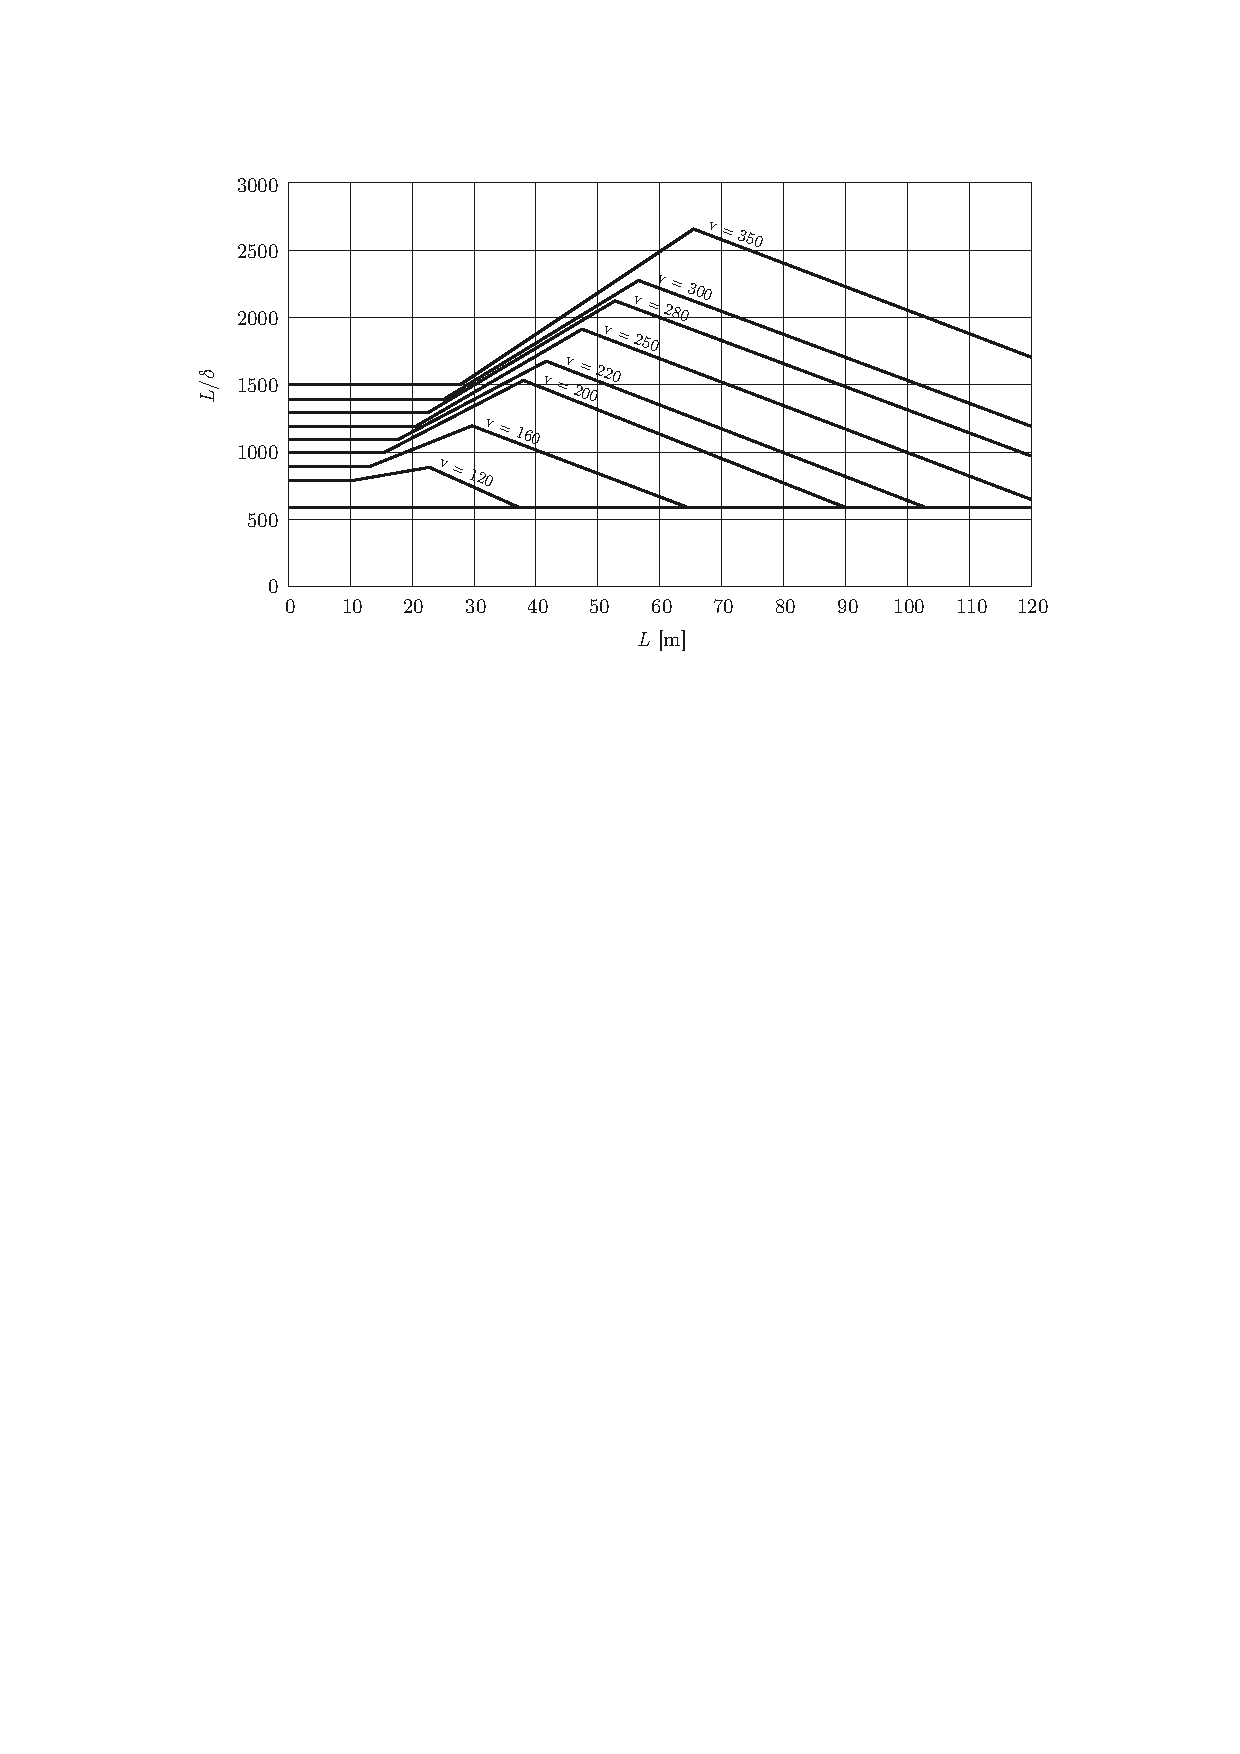
\includegraphics[]{/dynamic_railway/simp_comfort_class.pdf}
	\captionsetup{justification=centering}
	\caption{Nomogram do oceny komfortu w pojeździe na podstawie ugięć dla układu w postaci ciągu trzech przęseł swobodnie podpartych przy bardzo dobrym poziomie komfortu}
	\label{fig:simpl_comfort_clas}
\end{figure}

Obiekt kolejowy uznaje sią za poprawnie zaprojektowany jeśli spełnione są wszystkie Stany Graniczne Nośności i Użytkowania według PN-EN 1990 i PN-EN 1991-2, a w tym:  warunki nośności konstrukcji, trwałości zmęczeniowej, bezpieczeństwa nawierzchni kolejowej i wymagana klasa komfortu.

